\documentclass{article}
\usepackage{tikz}
\usetikzlibrary{matrix}
\usepackage[margin=1in]{geometry}
\begin{document}
% --- Frame 0 ---
\begin{center}\LARGE\textbf{Algorithm}\\[6mm]\end{center}
\begin{center}
\begin{flushleft}\textbf{Log}\\[1.75mm]\end{flushleft}
\begin{tikzpicture}
  \filldraw[fill=white!0, draw=none] (0,0) rectangle (10cm, -0.25cm);
\end{tikzpicture}
\end{center}
\noindent\rule{\linewidth}{0.3pt}
\begin{center}
\begin{flushleft}\textbf{Array}\\[1.75mm]\end{flushleft}
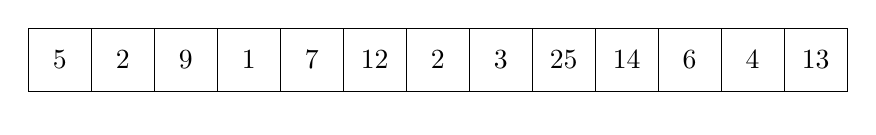
\begin{tikzpicture}
  \filldraw[fill=white!0, draw=none] (0cm,0cm) rectangle (10.4cm, -1cm);
  \filldraw[fill=white] (0cm,-0.8cm) rectangle (0.8cm,0cm);
  \node at (0.4cm,-0.4cm) {5};
  \filldraw[fill=white] (0.8cm,-0.8cm) rectangle (1.6cm,0cm);
  \node at (1.2000000000000002cm,-0.4cm) {2};
  \filldraw[fill=white] (1.6cm,-0.8cm) rectangle (2.4000000000000004cm,0cm);
  \node at (2cm,-0.4cm) {9};
  \filldraw[fill=white] (2.4000000000000004cm,-0.8cm) rectangle (3.2cm,0cm);
  \node at (2.8000000000000003cm,-0.4cm) {1};
  \filldraw[fill=white] (3.2cm,-0.8cm) rectangle (4cm,0cm);
  \node at (3.6cm,-0.4cm) {7};
  \filldraw[fill=white] (4cm,-0.8cm) rectangle (4.8cm,0cm);
  \node at (4.4cm,-0.4cm) {12};
  \filldraw[fill=white] (4.800000000000001cm,-0.8cm) rectangle (5.6000000000000005cm,0cm);
  \node at (5.200000000000001cm,-0.4cm) {2};
  \filldraw[fill=white] (5.6000000000000005cm,-0.8cm) rectangle (6.4cm,0cm);
  \node at (6.000000000000001cm,-0.4cm) {3};
  \filldraw[fill=white] (6.4cm,-0.8cm) rectangle (7.2cm,0cm);
  \node at (6.800000000000001cm,-0.4cm) {25};
  \filldraw[fill=white] (7.2cm,-0.8cm) rectangle (8cm,0cm);
  \node at (7.6000000000000005cm,-0.4cm) {14};
  \filldraw[fill=white] (8cm,-0.8cm) rectangle (8.8cm,0cm);
  \node at (8.4cm,-0.4cm) {6};
  \filldraw[fill=white] (8.8cm,-0.8cm) rectangle (9.600000000000001cm,0cm);
  \node at (9.200000000000001cm,-0.4cm) {4};
  \filldraw[fill=white] (9.600000000000001cm,-0.8cm) rectangle (10.400000000000002cm,0cm);
  \node at (10.000000000000002cm,-0.4cm) {13};
\end{tikzpicture}
\end{center}
\newpage
% --- Frame 1 ---
\begin{center}\LARGE\textbf{Algorithm}\\[6mm]\end{center}
\begin{center}
\begin{flushleft}\textbf{Log}\\[1.75mm]\end{flushleft}

\begin{tikzpicture}
  \filldraw[fill=white!0, draw=none] (0,0) rectangle (10cm, -0.25cm);
  \node[anchor=north, align=center, text=black] at (5cm,0) {\texttt{Comparing cells at index 0 and 1}};
\end{tikzpicture}
\end{center}
\noindent\rule{\linewidth}{0.3pt}
\begin{center}
\begin{flushleft}\textbf{Array}\\[1.75mm]\end{flushleft}
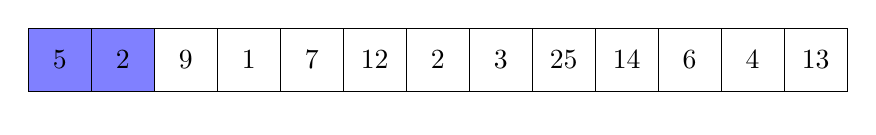
\begin{tikzpicture}
  \filldraw[fill=white!0, draw=none] (0cm,0cm) rectangle (10.4cm, -1cm);
  \filldraw[fill=blue!50] (0cm,-0.8cm) rectangle (0.8cm,0cm);
  \node at (0.4cm,-0.4cm) {5};
  \filldraw[fill=blue!50] (0.8cm,-0.8cm) rectangle (1.6cm,0cm);
  \node at (1.2000000000000002cm,-0.4cm) {2};
  \filldraw[fill=white] (1.6cm,-0.8cm) rectangle (2.4000000000000004cm,0cm);
  \node at (2cm,-0.4cm) {9};
  \filldraw[fill=white] (2.4000000000000004cm,-0.8cm) rectangle (3.2cm,0cm);
  \node at (2.8000000000000003cm,-0.4cm) {1};
  \filldraw[fill=white] (3.2cm,-0.8cm) rectangle (4cm,0cm);
  \node at (3.6cm,-0.4cm) {7};
  \filldraw[fill=white] (4cm,-0.8cm) rectangle (4.8cm,0cm);
  \node at (4.4cm,-0.4cm) {12};
  \filldraw[fill=white] (4.800000000000001cm,-0.8cm) rectangle (5.6000000000000005cm,0cm);
  \node at (5.200000000000001cm,-0.4cm) {2};
  \filldraw[fill=white] (5.6000000000000005cm,-0.8cm) rectangle (6.4cm,0cm);
  \node at (6.000000000000001cm,-0.4cm) {3};
  \filldraw[fill=white] (6.4cm,-0.8cm) rectangle (7.2cm,0cm);
  \node at (6.800000000000001cm,-0.4cm) {25};
  \filldraw[fill=white] (7.2cm,-0.8cm) rectangle (8cm,0cm);
  \node at (7.6000000000000005cm,-0.4cm) {14};
  \filldraw[fill=white] (8cm,-0.8cm) rectangle (8.8cm,0cm);
  \node at (8.4cm,-0.4cm) {6};
  \filldraw[fill=white] (8.8cm,-0.8cm) rectangle (9.600000000000001cm,0cm);
  \node at (9.200000000000001cm,-0.4cm) {4};
  \filldraw[fill=white] (9.600000000000001cm,-0.8cm) rectangle (10.400000000000002cm,0cm);
  \node at (10.000000000000002cm,-0.4cm) {13};
\end{tikzpicture}
\end{center}
\newpage
% --- Frame 2 ---
\begin{center}\LARGE\textbf{Algorithm}\\[6mm]\end{center}
\begin{center}
\begin{flushleft}\textbf{Log}\\[1.75mm]\end{flushleft}

\begin{tikzpicture}
  \filldraw[fill=white!0, draw=none] (0,0) rectangle (10cm, -0.25cm);
  \node[anchor=north, align=center, text=black] at (5cm,0) {\texttt{Swapping cells at index 0 and 1}};
\end{tikzpicture}
\end{center}
\noindent\rule{\linewidth}{0.3pt}
\begin{center}
\begin{flushleft}\textbf{Array}\\[1.75mm]\end{flushleft}
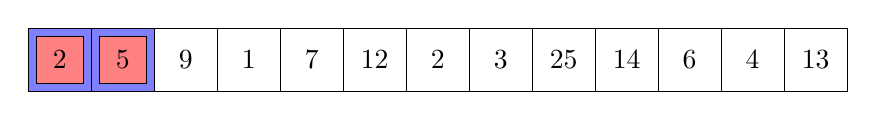
\begin{tikzpicture}
  \filldraw[fill=white!0, draw=none] (0cm,0cm) rectangle (10.4cm, -1cm);
  \filldraw[fill=blue!50] (0cm,-0.8cm) rectangle (0.8cm,0cm);
  \filldraw[fill=red!50] (0.1cm,-0.7000000000000001cm) rectangle (0.7000000000000001cm,-0.1cm);
  \node at (0.4cm,-0.4cm) {2};
  \filldraw[fill=blue!50] (0.8cm,-0.8cm) rectangle (1.6cm,0cm);
  \filldraw[fill=red!50] (0.9cm,-0.7000000000000001cm) rectangle (1.5cm,-0.1cm);
  \node at (1.2000000000000002cm,-0.4cm) {5};
  \filldraw[fill=white] (1.6cm,-0.8cm) rectangle (2.4000000000000004cm,0cm);
  \node at (2cm,-0.4cm) {9};
  \filldraw[fill=white] (2.4000000000000004cm,-0.8cm) rectangle (3.2cm,0cm);
  \node at (2.8000000000000003cm,-0.4cm) {1};
  \filldraw[fill=white] (3.2cm,-0.8cm) rectangle (4cm,0cm);
  \node at (3.6cm,-0.4cm) {7};
  \filldraw[fill=white] (4cm,-0.8cm) rectangle (4.8cm,0cm);
  \node at (4.4cm,-0.4cm) {12};
  \filldraw[fill=white] (4.800000000000001cm,-0.8cm) rectangle (5.6000000000000005cm,0cm);
  \node at (5.200000000000001cm,-0.4cm) {2};
  \filldraw[fill=white] (5.6000000000000005cm,-0.8cm) rectangle (6.4cm,0cm);
  \node at (6.000000000000001cm,-0.4cm) {3};
  \filldraw[fill=white] (6.4cm,-0.8cm) rectangle (7.2cm,0cm);
  \node at (6.800000000000001cm,-0.4cm) {25};
  \filldraw[fill=white] (7.2cm,-0.8cm) rectangle (8cm,0cm);
  \node at (7.6000000000000005cm,-0.4cm) {14};
  \filldraw[fill=white] (8cm,-0.8cm) rectangle (8.8cm,0cm);
  \node at (8.4cm,-0.4cm) {6};
  \filldraw[fill=white] (8.8cm,-0.8cm) rectangle (9.600000000000001cm,0cm);
  \node at (9.200000000000001cm,-0.4cm) {4};
  \filldraw[fill=white] (9.600000000000001cm,-0.8cm) rectangle (10.400000000000002cm,0cm);
  \node at (10.000000000000002cm,-0.4cm) {13};
\end{tikzpicture}
\end{center}
\newpage
% --- Frame 3 ---
\begin{center}\LARGE\textbf{Algorithm}\\[6mm]\end{center}
\begin{center}
\begin{flushleft}\textbf{Log}\\[1.75mm]\end{flushleft}

\begin{tikzpicture}
  \filldraw[fill=white!0, draw=none] (0,0) rectangle (10cm, -0.25cm);
  \node[anchor=north, align=center, text=black] at (5cm,0) {\texttt{Comparing cells at index 1 and 2}};
\end{tikzpicture}
\end{center}
\noindent\rule{\linewidth}{0.3pt}
\begin{center}
\begin{flushleft}\textbf{Array}\\[1.75mm]\end{flushleft}
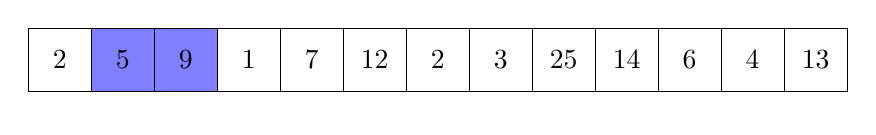
\begin{tikzpicture}
  \filldraw[fill=white!0, draw=none] (0cm,0cm) rectangle (10.4cm, -1cm);
  \filldraw[fill=white] (0cm,-0.8cm) rectangle (0.8cm,0cm);
  \node at (0.4cm,-0.4cm) {2};
  \filldraw[fill=blue!50] (0.8cm,-0.8cm) rectangle (1.6cm,0cm);
  \node at (1.2000000000000002cm,-0.4cm) {5};
  \filldraw[fill=blue!50] (1.6cm,-0.8cm) rectangle (2.4000000000000004cm,0cm);
  \node at (2cm,-0.4cm) {9};
  \filldraw[fill=white] (2.4000000000000004cm,-0.8cm) rectangle (3.2cm,0cm);
  \node at (2.8000000000000003cm,-0.4cm) {1};
  \filldraw[fill=white] (3.2cm,-0.8cm) rectangle (4cm,0cm);
  \node at (3.6cm,-0.4cm) {7};
  \filldraw[fill=white] (4cm,-0.8cm) rectangle (4.8cm,0cm);
  \node at (4.4cm,-0.4cm) {12};
  \filldraw[fill=white] (4.800000000000001cm,-0.8cm) rectangle (5.6000000000000005cm,0cm);
  \node at (5.200000000000001cm,-0.4cm) {2};
  \filldraw[fill=white] (5.6000000000000005cm,-0.8cm) rectangle (6.4cm,0cm);
  \node at (6.000000000000001cm,-0.4cm) {3};
  \filldraw[fill=white] (6.4cm,-0.8cm) rectangle (7.2cm,0cm);
  \node at (6.800000000000001cm,-0.4cm) {25};
  \filldraw[fill=white] (7.2cm,-0.8cm) rectangle (8cm,0cm);
  \node at (7.6000000000000005cm,-0.4cm) {14};
  \filldraw[fill=white] (8cm,-0.8cm) rectangle (8.8cm,0cm);
  \node at (8.4cm,-0.4cm) {6};
  \filldraw[fill=white] (8.8cm,-0.8cm) rectangle (9.600000000000001cm,0cm);
  \node at (9.200000000000001cm,-0.4cm) {4};
  \filldraw[fill=white] (9.600000000000001cm,-0.8cm) rectangle (10.400000000000002cm,0cm);
  \node at (10.000000000000002cm,-0.4cm) {13};
\end{tikzpicture}
\end{center}
\newpage
% --- Frame 4 ---
\begin{center}\LARGE\textbf{Algorithm}\\[6mm]\end{center}
\begin{center}
\begin{flushleft}\textbf{Log}\\[1.75mm]\end{flushleft}

\begin{tikzpicture}
  \filldraw[fill=white!0, draw=none] (0,0) rectangle (10cm, -0.25cm);
  \node[anchor=north, align=center, text=black] at (5cm,0) {\texttt{Comparing cells at index 2 and 3}};
\end{tikzpicture}
\end{center}
\noindent\rule{\linewidth}{0.3pt}
\begin{center}
\begin{flushleft}\textbf{Array}\\[1.75mm]\end{flushleft}
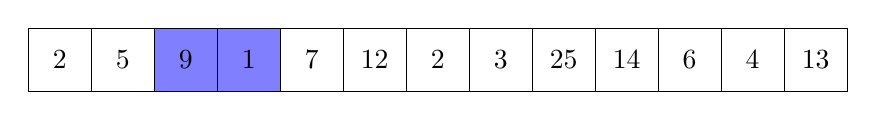
\begin{tikzpicture}
  \filldraw[fill=white!0, draw=none] (0cm,0cm) rectangle (10.4cm, -1cm);
  \filldraw[fill=white] (0cm,-0.8cm) rectangle (0.8cm,0cm);
  \node at (0.4cm,-0.4cm) {2};
  \filldraw[fill=white] (0.8cm,-0.8cm) rectangle (1.6cm,0cm);
  \node at (1.2000000000000002cm,-0.4cm) {5};
  \filldraw[fill=blue!50] (1.6cm,-0.8cm) rectangle (2.4000000000000004cm,0cm);
  \node at (2cm,-0.4cm) {9};
  \filldraw[fill=blue!50] (2.4000000000000004cm,-0.8cm) rectangle (3.2cm,0cm);
  \node at (2.8000000000000003cm,-0.4cm) {1};
  \filldraw[fill=white] (3.2cm,-0.8cm) rectangle (4cm,0cm);
  \node at (3.6cm,-0.4cm) {7};
  \filldraw[fill=white] (4cm,-0.8cm) rectangle (4.8cm,0cm);
  \node at (4.4cm,-0.4cm) {12};
  \filldraw[fill=white] (4.800000000000001cm,-0.8cm) rectangle (5.6000000000000005cm,0cm);
  \node at (5.200000000000001cm,-0.4cm) {2};
  \filldraw[fill=white] (5.6000000000000005cm,-0.8cm) rectangle (6.4cm,0cm);
  \node at (6.000000000000001cm,-0.4cm) {3};
  \filldraw[fill=white] (6.4cm,-0.8cm) rectangle (7.2cm,0cm);
  \node at (6.800000000000001cm,-0.4cm) {25};
  \filldraw[fill=white] (7.2cm,-0.8cm) rectangle (8cm,0cm);
  \node at (7.6000000000000005cm,-0.4cm) {14};
  \filldraw[fill=white] (8cm,-0.8cm) rectangle (8.8cm,0cm);
  \node at (8.4cm,-0.4cm) {6};
  \filldraw[fill=white] (8.8cm,-0.8cm) rectangle (9.600000000000001cm,0cm);
  \node at (9.200000000000001cm,-0.4cm) {4};
  \filldraw[fill=white] (9.600000000000001cm,-0.8cm) rectangle (10.400000000000002cm,0cm);
  \node at (10.000000000000002cm,-0.4cm) {13};
\end{tikzpicture}
\end{center}
\newpage
% --- Frame 5 ---
\begin{center}\LARGE\textbf{Algorithm}\\[6mm]\end{center}
\begin{center}
\begin{flushleft}\textbf{Log}\\[1.75mm]\end{flushleft}

\begin{tikzpicture}
  \filldraw[fill=white!0, draw=none] (0,0) rectangle (10cm, -0.25cm);
  \node[anchor=north, align=center, text=black] at (5cm,0) {\texttt{Swapping cells at index 2 and 3}};
\end{tikzpicture}
\end{center}
\noindent\rule{\linewidth}{0.3pt}
\begin{center}
\begin{flushleft}\textbf{Array}\\[1.75mm]\end{flushleft}
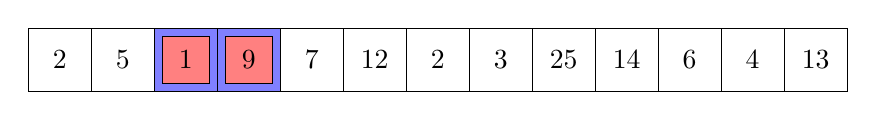
\begin{tikzpicture}
  \filldraw[fill=white!0, draw=none] (0cm,0cm) rectangle (10.4cm, -1cm);
  \filldraw[fill=white] (0cm,-0.8cm) rectangle (0.8cm,0cm);
  \node at (0.4cm,-0.4cm) {2};
  \filldraw[fill=white] (0.8cm,-0.8cm) rectangle (1.6cm,0cm);
  \node at (1.2000000000000002cm,-0.4cm) {5};
  \filldraw[fill=blue!50] (1.6cm,-0.8cm) rectangle (2.4000000000000004cm,0cm);
  \filldraw[fill=red!50] (1.7000000000000002cm,-0.7000000000000001cm) rectangle (2.3000000000000003cm,-0.1cm);
  \node at (2cm,-0.4cm) {1};
  \filldraw[fill=blue!50] (2.4000000000000004cm,-0.8cm) rectangle (3.2cm,0cm);
  \filldraw[fill=red!50] (2.5000000000000004cm,-0.7000000000000001cm) rectangle (3.1cm,-0.1cm);
  \node at (2.8000000000000003cm,-0.4cm) {9};
  \filldraw[fill=white] (3.2cm,-0.8cm) rectangle (4cm,0cm);
  \node at (3.6cm,-0.4cm) {7};
  \filldraw[fill=white] (4cm,-0.8cm) rectangle (4.8cm,0cm);
  \node at (4.4cm,-0.4cm) {12};
  \filldraw[fill=white] (4.800000000000001cm,-0.8cm) rectangle (5.6000000000000005cm,0cm);
  \node at (5.200000000000001cm,-0.4cm) {2};
  \filldraw[fill=white] (5.6000000000000005cm,-0.8cm) rectangle (6.4cm,0cm);
  \node at (6.000000000000001cm,-0.4cm) {3};
  \filldraw[fill=white] (6.4cm,-0.8cm) rectangle (7.2cm,0cm);
  \node at (6.800000000000001cm,-0.4cm) {25};
  \filldraw[fill=white] (7.2cm,-0.8cm) rectangle (8cm,0cm);
  \node at (7.6000000000000005cm,-0.4cm) {14};
  \filldraw[fill=white] (8cm,-0.8cm) rectangle (8.8cm,0cm);
  \node at (8.4cm,-0.4cm) {6};
  \filldraw[fill=white] (8.8cm,-0.8cm) rectangle (9.600000000000001cm,0cm);
  \node at (9.200000000000001cm,-0.4cm) {4};
  \filldraw[fill=white] (9.600000000000001cm,-0.8cm) rectangle (10.400000000000002cm,0cm);
  \node at (10.000000000000002cm,-0.4cm) {13};
\end{tikzpicture}
\end{center}
\newpage
% --- Frame 6 ---
\begin{center}\LARGE\textbf{Algorithm}\\[6mm]\end{center}
\begin{center}
\begin{flushleft}\textbf{Log}\\[1.75mm]\end{flushleft}

\begin{tikzpicture}
  \filldraw[fill=white!0, draw=none] (0,0) rectangle (10cm, -0.25cm);
  \node[anchor=north, align=center, text=black] at (5cm,0) {\texttt{Comparing cells at index 3 and 4}};
\end{tikzpicture}
\end{center}
\noindent\rule{\linewidth}{0.3pt}
\begin{center}
\begin{flushleft}\textbf{Array}\\[1.75mm]\end{flushleft}
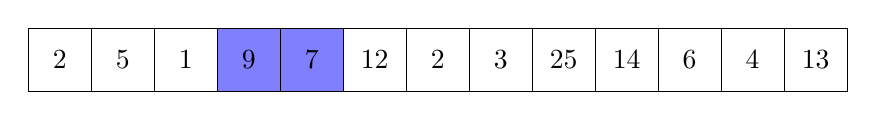
\begin{tikzpicture}
  \filldraw[fill=white!0, draw=none] (0cm,0cm) rectangle (10.4cm, -1cm);
  \filldraw[fill=white] (0cm,-0.8cm) rectangle (0.8cm,0cm);
  \node at (0.4cm,-0.4cm) {2};
  \filldraw[fill=white] (0.8cm,-0.8cm) rectangle (1.6cm,0cm);
  \node at (1.2000000000000002cm,-0.4cm) {5};
  \filldraw[fill=white] (1.6cm,-0.8cm) rectangle (2.4000000000000004cm,0cm);
  \node at (2cm,-0.4cm) {1};
  \filldraw[fill=blue!50] (2.4000000000000004cm,-0.8cm) rectangle (3.2cm,0cm);
  \node at (2.8000000000000003cm,-0.4cm) {9};
  \filldraw[fill=blue!50] (3.2cm,-0.8cm) rectangle (4cm,0cm);
  \node at (3.6cm,-0.4cm) {7};
  \filldraw[fill=white] (4cm,-0.8cm) rectangle (4.8cm,0cm);
  \node at (4.4cm,-0.4cm) {12};
  \filldraw[fill=white] (4.800000000000001cm,-0.8cm) rectangle (5.6000000000000005cm,0cm);
  \node at (5.200000000000001cm,-0.4cm) {2};
  \filldraw[fill=white] (5.6000000000000005cm,-0.8cm) rectangle (6.4cm,0cm);
  \node at (6.000000000000001cm,-0.4cm) {3};
  \filldraw[fill=white] (6.4cm,-0.8cm) rectangle (7.2cm,0cm);
  \node at (6.800000000000001cm,-0.4cm) {25};
  \filldraw[fill=white] (7.2cm,-0.8cm) rectangle (8cm,0cm);
  \node at (7.6000000000000005cm,-0.4cm) {14};
  \filldraw[fill=white] (8cm,-0.8cm) rectangle (8.8cm,0cm);
  \node at (8.4cm,-0.4cm) {6};
  \filldraw[fill=white] (8.8cm,-0.8cm) rectangle (9.600000000000001cm,0cm);
  \node at (9.200000000000001cm,-0.4cm) {4};
  \filldraw[fill=white] (9.600000000000001cm,-0.8cm) rectangle (10.400000000000002cm,0cm);
  \node at (10.000000000000002cm,-0.4cm) {13};
\end{tikzpicture}
\end{center}
\newpage
% --- Frame 7 ---
\begin{center}\LARGE\textbf{Algorithm}\\[6mm]\end{center}
\begin{center}
\begin{flushleft}\textbf{Log}\\[1.75mm]\end{flushleft}

\begin{tikzpicture}
  \filldraw[fill=white!0, draw=none] (0,0) rectangle (10cm, -0.25cm);
  \node[anchor=north, align=center, text=black] at (5cm,0) {\texttt{Swapping cells at index 3 and 4}};
\end{tikzpicture}
\end{center}
\noindent\rule{\linewidth}{0.3pt}
\begin{center}
\begin{flushleft}\textbf{Array}\\[1.75mm]\end{flushleft}
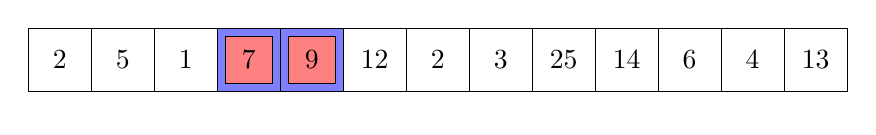
\begin{tikzpicture}
  \filldraw[fill=white!0, draw=none] (0cm,0cm) rectangle (10.4cm, -1cm);
  \filldraw[fill=white] (0cm,-0.8cm) rectangle (0.8cm,0cm);
  \node at (0.4cm,-0.4cm) {2};
  \filldraw[fill=white] (0.8cm,-0.8cm) rectangle (1.6cm,0cm);
  \node at (1.2000000000000002cm,-0.4cm) {5};
  \filldraw[fill=white] (1.6cm,-0.8cm) rectangle (2.4000000000000004cm,0cm);
  \node at (2cm,-0.4cm) {1};
  \filldraw[fill=blue!50] (2.4000000000000004cm,-0.8cm) rectangle (3.2cm,0cm);
  \filldraw[fill=red!50] (2.5000000000000004cm,-0.7000000000000001cm) rectangle (3.1cm,-0.1cm);
  \node at (2.8000000000000003cm,-0.4cm) {7};
  \filldraw[fill=blue!50] (3.2cm,-0.8cm) rectangle (4cm,0cm);
  \filldraw[fill=red!50] (3.3000000000000003cm,-0.7000000000000001cm) rectangle (3.9cm,-0.1cm);
  \node at (3.6cm,-0.4cm) {9};
  \filldraw[fill=white] (4cm,-0.8cm) rectangle (4.8cm,0cm);
  \node at (4.4cm,-0.4cm) {12};
  \filldraw[fill=white] (4.800000000000001cm,-0.8cm) rectangle (5.6000000000000005cm,0cm);
  \node at (5.200000000000001cm,-0.4cm) {2};
  \filldraw[fill=white] (5.6000000000000005cm,-0.8cm) rectangle (6.4cm,0cm);
  \node at (6.000000000000001cm,-0.4cm) {3};
  \filldraw[fill=white] (6.4cm,-0.8cm) rectangle (7.2cm,0cm);
  \node at (6.800000000000001cm,-0.4cm) {25};
  \filldraw[fill=white] (7.2cm,-0.8cm) rectangle (8cm,0cm);
  \node at (7.6000000000000005cm,-0.4cm) {14};
  \filldraw[fill=white] (8cm,-0.8cm) rectangle (8.8cm,0cm);
  \node at (8.4cm,-0.4cm) {6};
  \filldraw[fill=white] (8.8cm,-0.8cm) rectangle (9.600000000000001cm,0cm);
  \node at (9.200000000000001cm,-0.4cm) {4};
  \filldraw[fill=white] (9.600000000000001cm,-0.8cm) rectangle (10.400000000000002cm,0cm);
  \node at (10.000000000000002cm,-0.4cm) {13};
\end{tikzpicture}
\end{center}
\newpage
% --- Frame 8 ---
\begin{center}\LARGE\textbf{Algorithm}\\[6mm]\end{center}
\begin{center}
\begin{flushleft}\textbf{Log}\\[1.75mm]\end{flushleft}

\begin{tikzpicture}
  \filldraw[fill=white!0, draw=none] (0,0) rectangle (10cm, -0.25cm);
  \node[anchor=north, align=center, text=black] at (5cm,0) {\texttt{Comparing cells at index 4 and 5}};
\end{tikzpicture}
\end{center}
\noindent\rule{\linewidth}{0.3pt}
\begin{center}
\begin{flushleft}\textbf{Array}\\[1.75mm]\end{flushleft}
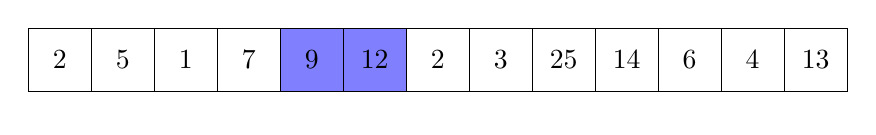
\begin{tikzpicture}
  \filldraw[fill=white!0, draw=none] (0cm,0cm) rectangle (10.4cm, -1cm);
  \filldraw[fill=white] (0cm,-0.8cm) rectangle (0.8cm,0cm);
  \node at (0.4cm,-0.4cm) {2};
  \filldraw[fill=white] (0.8cm,-0.8cm) rectangle (1.6cm,0cm);
  \node at (1.2000000000000002cm,-0.4cm) {5};
  \filldraw[fill=white] (1.6cm,-0.8cm) rectangle (2.4000000000000004cm,0cm);
  \node at (2cm,-0.4cm) {1};
  \filldraw[fill=white] (2.4000000000000004cm,-0.8cm) rectangle (3.2cm,0cm);
  \node at (2.8000000000000003cm,-0.4cm) {7};
  \filldraw[fill=blue!50] (3.2cm,-0.8cm) rectangle (4cm,0cm);
  \node at (3.6cm,-0.4cm) {9};
  \filldraw[fill=blue!50] (4cm,-0.8cm) rectangle (4.8cm,0cm);
  \node at (4.4cm,-0.4cm) {12};
  \filldraw[fill=white] (4.800000000000001cm,-0.8cm) rectangle (5.6000000000000005cm,0cm);
  \node at (5.200000000000001cm,-0.4cm) {2};
  \filldraw[fill=white] (5.6000000000000005cm,-0.8cm) rectangle (6.4cm,0cm);
  \node at (6.000000000000001cm,-0.4cm) {3};
  \filldraw[fill=white] (6.4cm,-0.8cm) rectangle (7.2cm,0cm);
  \node at (6.800000000000001cm,-0.4cm) {25};
  \filldraw[fill=white] (7.2cm,-0.8cm) rectangle (8cm,0cm);
  \node at (7.6000000000000005cm,-0.4cm) {14};
  \filldraw[fill=white] (8cm,-0.8cm) rectangle (8.8cm,0cm);
  \node at (8.4cm,-0.4cm) {6};
  \filldraw[fill=white] (8.8cm,-0.8cm) rectangle (9.600000000000001cm,0cm);
  \node at (9.200000000000001cm,-0.4cm) {4};
  \filldraw[fill=white] (9.600000000000001cm,-0.8cm) rectangle (10.400000000000002cm,0cm);
  \node at (10.000000000000002cm,-0.4cm) {13};
\end{tikzpicture}
\end{center}
\newpage
% --- Frame 9 ---
\begin{center}\LARGE\textbf{Algorithm}\\[6mm]\end{center}
\begin{center}
\begin{flushleft}\textbf{Log}\\[1.75mm]\end{flushleft}

\begin{tikzpicture}
  \filldraw[fill=white!0, draw=none] (0,0) rectangle (10cm, -0.25cm);
  \node[anchor=north, align=center, text=black] at (5cm,0) {\texttt{Comparing cells at index 5 and 6}};
\end{tikzpicture}
\end{center}
\noindent\rule{\linewidth}{0.3pt}
\begin{center}
\begin{flushleft}\textbf{Array}\\[1.75mm]\end{flushleft}
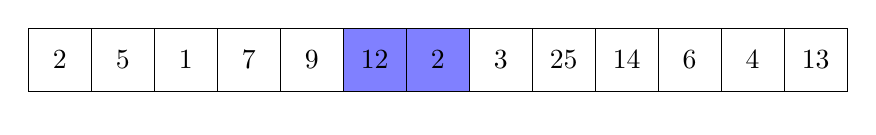
\begin{tikzpicture}
  \filldraw[fill=white!0, draw=none] (0cm,0cm) rectangle (10.4cm, -1cm);
  \filldraw[fill=white] (0cm,-0.8cm) rectangle (0.8cm,0cm);
  \node at (0.4cm,-0.4cm) {2};
  \filldraw[fill=white] (0.8cm,-0.8cm) rectangle (1.6cm,0cm);
  \node at (1.2000000000000002cm,-0.4cm) {5};
  \filldraw[fill=white] (1.6cm,-0.8cm) rectangle (2.4000000000000004cm,0cm);
  \node at (2cm,-0.4cm) {1};
  \filldraw[fill=white] (2.4000000000000004cm,-0.8cm) rectangle (3.2cm,0cm);
  \node at (2.8000000000000003cm,-0.4cm) {7};
  \filldraw[fill=white] (3.2cm,-0.8cm) rectangle (4cm,0cm);
  \node at (3.6cm,-0.4cm) {9};
  \filldraw[fill=blue!50] (4cm,-0.8cm) rectangle (4.8cm,0cm);
  \node at (4.4cm,-0.4cm) {12};
  \filldraw[fill=blue!50] (4.800000000000001cm,-0.8cm) rectangle (5.6000000000000005cm,0cm);
  \node at (5.200000000000001cm,-0.4cm) {2};
  \filldraw[fill=white] (5.6000000000000005cm,-0.8cm) rectangle (6.4cm,0cm);
  \node at (6.000000000000001cm,-0.4cm) {3};
  \filldraw[fill=white] (6.4cm,-0.8cm) rectangle (7.2cm,0cm);
  \node at (6.800000000000001cm,-0.4cm) {25};
  \filldraw[fill=white] (7.2cm,-0.8cm) rectangle (8cm,0cm);
  \node at (7.6000000000000005cm,-0.4cm) {14};
  \filldraw[fill=white] (8cm,-0.8cm) rectangle (8.8cm,0cm);
  \node at (8.4cm,-0.4cm) {6};
  \filldraw[fill=white] (8.8cm,-0.8cm) rectangle (9.600000000000001cm,0cm);
  \node at (9.200000000000001cm,-0.4cm) {4};
  \filldraw[fill=white] (9.600000000000001cm,-0.8cm) rectangle (10.400000000000002cm,0cm);
  \node at (10.000000000000002cm,-0.4cm) {13};
\end{tikzpicture}
\end{center}
\newpage
% --- Frame 10 ---
\begin{center}\LARGE\textbf{Algorithm}\\[6mm]\end{center}
\begin{center}
\begin{flushleft}\textbf{Log}\\[1.75mm]\end{flushleft}

\begin{tikzpicture}
  \filldraw[fill=white!0, draw=none] (0,0) rectangle (10cm, -0.25cm);
  \node[anchor=north, align=center, text=black] at (5cm,0) {\texttt{Swapping cells at index 5 and 6}};
\end{tikzpicture}
\end{center}
\noindent\rule{\linewidth}{0.3pt}
\begin{center}
\begin{flushleft}\textbf{Array}\\[1.75mm]\end{flushleft}
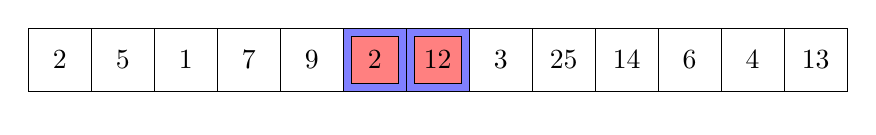
\begin{tikzpicture}
  \filldraw[fill=white!0, draw=none] (0cm,0cm) rectangle (10.4cm, -1cm);
  \filldraw[fill=white] (0cm,-0.8cm) rectangle (0.8cm,0cm);
  \node at (0.4cm,-0.4cm) {2};
  \filldraw[fill=white] (0.8cm,-0.8cm) rectangle (1.6cm,0cm);
  \node at (1.2000000000000002cm,-0.4cm) {5};
  \filldraw[fill=white] (1.6cm,-0.8cm) rectangle (2.4000000000000004cm,0cm);
  \node at (2cm,-0.4cm) {1};
  \filldraw[fill=white] (2.4000000000000004cm,-0.8cm) rectangle (3.2cm,0cm);
  \node at (2.8000000000000003cm,-0.4cm) {7};
  \filldraw[fill=white] (3.2cm,-0.8cm) rectangle (4cm,0cm);
  \node at (3.6cm,-0.4cm) {9};
  \filldraw[fill=blue!50] (4cm,-0.8cm) rectangle (4.8cm,0cm);
  \filldraw[fill=red!50] (4.1cm,-0.7000000000000001cm) rectangle (4.7cm,-0.1cm);
  \node at (4.4cm,-0.4cm) {2};
  \filldraw[fill=blue!50] (4.800000000000001cm,-0.8cm) rectangle (5.6000000000000005cm,0cm);
  \filldraw[fill=red!50] (4.9cm,-0.7000000000000001cm) rectangle (5.500000000000001cm,-0.1cm);
  \node at (5.200000000000001cm,-0.4cm) {12};
  \filldraw[fill=white] (5.6000000000000005cm,-0.8cm) rectangle (6.4cm,0cm);
  \node at (6.000000000000001cm,-0.4cm) {3};
  \filldraw[fill=white] (6.4cm,-0.8cm) rectangle (7.2cm,0cm);
  \node at (6.800000000000001cm,-0.4cm) {25};
  \filldraw[fill=white] (7.2cm,-0.8cm) rectangle (8cm,0cm);
  \node at (7.6000000000000005cm,-0.4cm) {14};
  \filldraw[fill=white] (8cm,-0.8cm) rectangle (8.8cm,0cm);
  \node at (8.4cm,-0.4cm) {6};
  \filldraw[fill=white] (8.8cm,-0.8cm) rectangle (9.600000000000001cm,0cm);
  \node at (9.200000000000001cm,-0.4cm) {4};
  \filldraw[fill=white] (9.600000000000001cm,-0.8cm) rectangle (10.400000000000002cm,0cm);
  \node at (10.000000000000002cm,-0.4cm) {13};
\end{tikzpicture}
\end{center}
\newpage
% --- Frame 11 ---
\begin{center}\LARGE\textbf{Algorithm}\\[6mm]\end{center}
\begin{center}
\begin{flushleft}\textbf{Log}\\[1.75mm]\end{flushleft}

\begin{tikzpicture}
  \filldraw[fill=white!0, draw=none] (0,0) rectangle (10cm, -0.25cm);
  \node[anchor=north, align=center, text=black] at (5cm,0) {\texttt{Comparing cells at index 6 and 7}};
\end{tikzpicture}
\end{center}
\noindent\rule{\linewidth}{0.3pt}
\begin{center}
\begin{flushleft}\textbf{Array}\\[1.75mm]\end{flushleft}
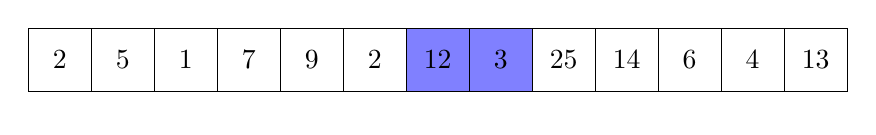
\begin{tikzpicture}
  \filldraw[fill=white!0, draw=none] (0cm,0cm) rectangle (10.4cm, -1cm);
  \filldraw[fill=white] (0cm,-0.8cm) rectangle (0.8cm,0cm);
  \node at (0.4cm,-0.4cm) {2};
  \filldraw[fill=white] (0.8cm,-0.8cm) rectangle (1.6cm,0cm);
  \node at (1.2000000000000002cm,-0.4cm) {5};
  \filldraw[fill=white] (1.6cm,-0.8cm) rectangle (2.4000000000000004cm,0cm);
  \node at (2cm,-0.4cm) {1};
  \filldraw[fill=white] (2.4000000000000004cm,-0.8cm) rectangle (3.2cm,0cm);
  \node at (2.8000000000000003cm,-0.4cm) {7};
  \filldraw[fill=white] (3.2cm,-0.8cm) rectangle (4cm,0cm);
  \node at (3.6cm,-0.4cm) {9};
  \filldraw[fill=white] (4cm,-0.8cm) rectangle (4.8cm,0cm);
  \node at (4.4cm,-0.4cm) {2};
  \filldraw[fill=blue!50] (4.800000000000001cm,-0.8cm) rectangle (5.6000000000000005cm,0cm);
  \node at (5.200000000000001cm,-0.4cm) {12};
  \filldraw[fill=blue!50] (5.6000000000000005cm,-0.8cm) rectangle (6.4cm,0cm);
  \node at (6.000000000000001cm,-0.4cm) {3};
  \filldraw[fill=white] (6.4cm,-0.8cm) rectangle (7.2cm,0cm);
  \node at (6.800000000000001cm,-0.4cm) {25};
  \filldraw[fill=white] (7.2cm,-0.8cm) rectangle (8cm,0cm);
  \node at (7.6000000000000005cm,-0.4cm) {14};
  \filldraw[fill=white] (8cm,-0.8cm) rectangle (8.8cm,0cm);
  \node at (8.4cm,-0.4cm) {6};
  \filldraw[fill=white] (8.8cm,-0.8cm) rectangle (9.600000000000001cm,0cm);
  \node at (9.200000000000001cm,-0.4cm) {4};
  \filldraw[fill=white] (9.600000000000001cm,-0.8cm) rectangle (10.400000000000002cm,0cm);
  \node at (10.000000000000002cm,-0.4cm) {13};
\end{tikzpicture}
\end{center}
\newpage
% --- Frame 12 ---
\begin{center}\LARGE\textbf{Algorithm}\\[6mm]\end{center}
\begin{center}
\begin{flushleft}\textbf{Log}\\[1.75mm]\end{flushleft}

\begin{tikzpicture}
  \filldraw[fill=white!0, draw=none] (0,0) rectangle (10cm, -0.25cm);
  \node[anchor=north, align=center, text=black] at (5cm,0) {\texttt{Swapping cells at index 6 and 7}};
\end{tikzpicture}
\end{center}
\noindent\rule{\linewidth}{0.3pt}
\begin{center}
\begin{flushleft}\textbf{Array}\\[1.75mm]\end{flushleft}
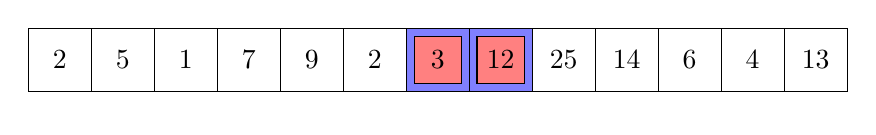
\begin{tikzpicture}
  \filldraw[fill=white!0, draw=none] (0cm,0cm) rectangle (10.4cm, -1cm);
  \filldraw[fill=white] (0cm,-0.8cm) rectangle (0.8cm,0cm);
  \node at (0.4cm,-0.4cm) {2};
  \filldraw[fill=white] (0.8cm,-0.8cm) rectangle (1.6cm,0cm);
  \node at (1.2000000000000002cm,-0.4cm) {5};
  \filldraw[fill=white] (1.6cm,-0.8cm) rectangle (2.4000000000000004cm,0cm);
  \node at (2cm,-0.4cm) {1};
  \filldraw[fill=white] (2.4000000000000004cm,-0.8cm) rectangle (3.2cm,0cm);
  \node at (2.8000000000000003cm,-0.4cm) {7};
  \filldraw[fill=white] (3.2cm,-0.8cm) rectangle (4cm,0cm);
  \node at (3.6cm,-0.4cm) {9};
  \filldraw[fill=white] (4cm,-0.8cm) rectangle (4.8cm,0cm);
  \node at (4.4cm,-0.4cm) {2};
  \filldraw[fill=blue!50] (4.800000000000001cm,-0.8cm) rectangle (5.6000000000000005cm,0cm);
  \filldraw[fill=red!50] (4.9cm,-0.7000000000000001cm) rectangle (5.500000000000001cm,-0.1cm);
  \node at (5.200000000000001cm,-0.4cm) {3};
  \filldraw[fill=blue!50] (5.6000000000000005cm,-0.8cm) rectangle (6.4cm,0cm);
  \filldraw[fill=red!50] (5.7cm,-0.7000000000000001cm) rectangle (6.300000000000001cm,-0.1cm);
  \node at (6.000000000000001cm,-0.4cm) {12};
  \filldraw[fill=white] (6.4cm,-0.8cm) rectangle (7.2cm,0cm);
  \node at (6.800000000000001cm,-0.4cm) {25};
  \filldraw[fill=white] (7.2cm,-0.8cm) rectangle (8cm,0cm);
  \node at (7.6000000000000005cm,-0.4cm) {14};
  \filldraw[fill=white] (8cm,-0.8cm) rectangle (8.8cm,0cm);
  \node at (8.4cm,-0.4cm) {6};
  \filldraw[fill=white] (8.8cm,-0.8cm) rectangle (9.600000000000001cm,0cm);
  \node at (9.200000000000001cm,-0.4cm) {4};
  \filldraw[fill=white] (9.600000000000001cm,-0.8cm) rectangle (10.400000000000002cm,0cm);
  \node at (10.000000000000002cm,-0.4cm) {13};
\end{tikzpicture}
\end{center}
\newpage
% --- Frame 13 ---
\begin{center}\LARGE\textbf{Algorithm}\\[6mm]\end{center}
\begin{center}
\begin{flushleft}\textbf{Log}\\[1.75mm]\end{flushleft}

\begin{tikzpicture}
  \filldraw[fill=white!0, draw=none] (0,0) rectangle (10cm, -0.25cm);
  \node[anchor=north, align=center, text=black] at (5cm,0) {\texttt{Comparing cells at index 7 and 8}};
\end{tikzpicture}
\end{center}
\noindent\rule{\linewidth}{0.3pt}
\begin{center}
\begin{flushleft}\textbf{Array}\\[1.75mm]\end{flushleft}
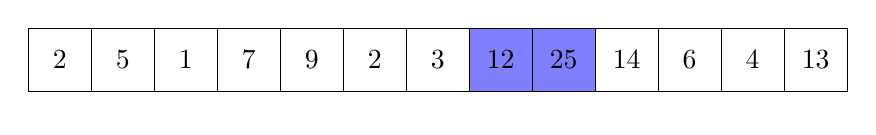
\begin{tikzpicture}
  \filldraw[fill=white!0, draw=none] (0cm,0cm) rectangle (10.4cm, -1cm);
  \filldraw[fill=white] (0cm,-0.8cm) rectangle (0.8cm,0cm);
  \node at (0.4cm,-0.4cm) {2};
  \filldraw[fill=white] (0.8cm,-0.8cm) rectangle (1.6cm,0cm);
  \node at (1.2000000000000002cm,-0.4cm) {5};
  \filldraw[fill=white] (1.6cm,-0.8cm) rectangle (2.4000000000000004cm,0cm);
  \node at (2cm,-0.4cm) {1};
  \filldraw[fill=white] (2.4000000000000004cm,-0.8cm) rectangle (3.2cm,0cm);
  \node at (2.8000000000000003cm,-0.4cm) {7};
  \filldraw[fill=white] (3.2cm,-0.8cm) rectangle (4cm,0cm);
  \node at (3.6cm,-0.4cm) {9};
  \filldraw[fill=white] (4cm,-0.8cm) rectangle (4.8cm,0cm);
  \node at (4.4cm,-0.4cm) {2};
  \filldraw[fill=white] (4.800000000000001cm,-0.8cm) rectangle (5.6000000000000005cm,0cm);
  \node at (5.200000000000001cm,-0.4cm) {3};
  \filldraw[fill=blue!50] (5.6000000000000005cm,-0.8cm) rectangle (6.4cm,0cm);
  \node at (6.000000000000001cm,-0.4cm) {12};
  \filldraw[fill=blue!50] (6.4cm,-0.8cm) rectangle (7.2cm,0cm);
  \node at (6.800000000000001cm,-0.4cm) {25};
  \filldraw[fill=white] (7.2cm,-0.8cm) rectangle (8cm,0cm);
  \node at (7.6000000000000005cm,-0.4cm) {14};
  \filldraw[fill=white] (8cm,-0.8cm) rectangle (8.8cm,0cm);
  \node at (8.4cm,-0.4cm) {6};
  \filldraw[fill=white] (8.8cm,-0.8cm) rectangle (9.600000000000001cm,0cm);
  \node at (9.200000000000001cm,-0.4cm) {4};
  \filldraw[fill=white] (9.600000000000001cm,-0.8cm) rectangle (10.400000000000002cm,0cm);
  \node at (10.000000000000002cm,-0.4cm) {13};
\end{tikzpicture}
\end{center}
\newpage
% --- Frame 14 ---
\begin{center}\LARGE\textbf{Algorithm}\\[6mm]\end{center}
\begin{center}
\begin{flushleft}\textbf{Log}\\[1.75mm]\end{flushleft}

\begin{tikzpicture}
  \filldraw[fill=white!0, draw=none] (0,0) rectangle (10cm, -0.25cm);
  \node[anchor=north, align=center, text=black] at (5cm,0) {\texttt{Comparing cells at index 8 and 9}};
\end{tikzpicture}
\end{center}
\noindent\rule{\linewidth}{0.3pt}
\begin{center}
\begin{flushleft}\textbf{Array}\\[1.75mm]\end{flushleft}
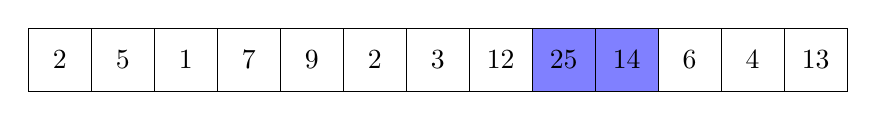
\begin{tikzpicture}
  \filldraw[fill=white!0, draw=none] (0cm,0cm) rectangle (10.4cm, -1cm);
  \filldraw[fill=white] (0cm,-0.8cm) rectangle (0.8cm,0cm);
  \node at (0.4cm,-0.4cm) {2};
  \filldraw[fill=white] (0.8cm,-0.8cm) rectangle (1.6cm,0cm);
  \node at (1.2000000000000002cm,-0.4cm) {5};
  \filldraw[fill=white] (1.6cm,-0.8cm) rectangle (2.4000000000000004cm,0cm);
  \node at (2cm,-0.4cm) {1};
  \filldraw[fill=white] (2.4000000000000004cm,-0.8cm) rectangle (3.2cm,0cm);
  \node at (2.8000000000000003cm,-0.4cm) {7};
  \filldraw[fill=white] (3.2cm,-0.8cm) rectangle (4cm,0cm);
  \node at (3.6cm,-0.4cm) {9};
  \filldraw[fill=white] (4cm,-0.8cm) rectangle (4.8cm,0cm);
  \node at (4.4cm,-0.4cm) {2};
  \filldraw[fill=white] (4.800000000000001cm,-0.8cm) rectangle (5.6000000000000005cm,0cm);
  \node at (5.200000000000001cm,-0.4cm) {3};
  \filldraw[fill=white] (5.6000000000000005cm,-0.8cm) rectangle (6.4cm,0cm);
  \node at (6.000000000000001cm,-0.4cm) {12};
  \filldraw[fill=blue!50] (6.4cm,-0.8cm) rectangle (7.2cm,0cm);
  \node at (6.800000000000001cm,-0.4cm) {25};
  \filldraw[fill=blue!50] (7.2cm,-0.8cm) rectangle (8cm,0cm);
  \node at (7.6000000000000005cm,-0.4cm) {14};
  \filldraw[fill=white] (8cm,-0.8cm) rectangle (8.8cm,0cm);
  \node at (8.4cm,-0.4cm) {6};
  \filldraw[fill=white] (8.8cm,-0.8cm) rectangle (9.600000000000001cm,0cm);
  \node at (9.200000000000001cm,-0.4cm) {4};
  \filldraw[fill=white] (9.600000000000001cm,-0.8cm) rectangle (10.400000000000002cm,0cm);
  \node at (10.000000000000002cm,-0.4cm) {13};
\end{tikzpicture}
\end{center}
\newpage
% --- Frame 15 ---
\begin{center}\LARGE\textbf{Algorithm}\\[6mm]\end{center}
\begin{center}
\begin{flushleft}\textbf{Log}\\[1.75mm]\end{flushleft}

\begin{tikzpicture}
  \filldraw[fill=white!0, draw=none] (0,0) rectangle (10cm, -0.25cm);
  \node[anchor=north, align=center, text=black] at (5cm,0) {\texttt{Swapping cells at index 8 and 9}};
\end{tikzpicture}
\end{center}
\noindent\rule{\linewidth}{0.3pt}
\begin{center}
\begin{flushleft}\textbf{Array}\\[1.75mm]\end{flushleft}
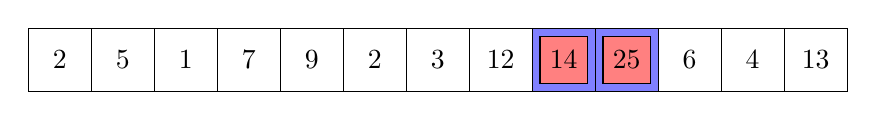
\begin{tikzpicture}
  \filldraw[fill=white!0, draw=none] (0cm,0cm) rectangle (10.4cm, -1cm);
  \filldraw[fill=white] (0cm,-0.8cm) rectangle (0.8cm,0cm);
  \node at (0.4cm,-0.4cm) {2};
  \filldraw[fill=white] (0.8cm,-0.8cm) rectangle (1.6cm,0cm);
  \node at (1.2000000000000002cm,-0.4cm) {5};
  \filldraw[fill=white] (1.6cm,-0.8cm) rectangle (2.4000000000000004cm,0cm);
  \node at (2cm,-0.4cm) {1};
  \filldraw[fill=white] (2.4000000000000004cm,-0.8cm) rectangle (3.2cm,0cm);
  \node at (2.8000000000000003cm,-0.4cm) {7};
  \filldraw[fill=white] (3.2cm,-0.8cm) rectangle (4cm,0cm);
  \node at (3.6cm,-0.4cm) {9};
  \filldraw[fill=white] (4cm,-0.8cm) rectangle (4.8cm,0cm);
  \node at (4.4cm,-0.4cm) {2};
  \filldraw[fill=white] (4.800000000000001cm,-0.8cm) rectangle (5.6000000000000005cm,0cm);
  \node at (5.200000000000001cm,-0.4cm) {3};
  \filldraw[fill=white] (5.6000000000000005cm,-0.8cm) rectangle (6.4cm,0cm);
  \node at (6.000000000000001cm,-0.4cm) {12};
  \filldraw[fill=blue!50] (6.4cm,-0.8cm) rectangle (7.2cm,0cm);
  \filldraw[fill=red!50] (6.5cm,-0.7000000000000001cm) rectangle (7.1000000000000005cm,-0.1cm);
  \node at (6.800000000000001cm,-0.4cm) {14};
  \filldraw[fill=blue!50] (7.2cm,-0.8cm) rectangle (8cm,0cm);
  \filldraw[fill=red!50] (7.3cm,-0.7000000000000001cm) rectangle (7.9cm,-0.1cm);
  \node at (7.6000000000000005cm,-0.4cm) {25};
  \filldraw[fill=white] (8cm,-0.8cm) rectangle (8.8cm,0cm);
  \node at (8.4cm,-0.4cm) {6};
  \filldraw[fill=white] (8.8cm,-0.8cm) rectangle (9.600000000000001cm,0cm);
  \node at (9.200000000000001cm,-0.4cm) {4};
  \filldraw[fill=white] (9.600000000000001cm,-0.8cm) rectangle (10.400000000000002cm,0cm);
  \node at (10.000000000000002cm,-0.4cm) {13};
\end{tikzpicture}
\end{center}
\newpage
% --- Frame 16 ---
\begin{center}\LARGE\textbf{Algorithm}\\[6mm]\end{center}
\begin{center}
\begin{flushleft}\textbf{Log}\\[1.75mm]\end{flushleft}

\begin{tikzpicture}
  \filldraw[fill=white!0, draw=none] (0,0) rectangle (10cm, -0.25cm);
  \node[anchor=north, align=center, text=black] at (5cm,0) {\texttt{Comparing cells at index 9 and 10}};
\end{tikzpicture}
\end{center}
\noindent\rule{\linewidth}{0.3pt}
\begin{center}
\begin{flushleft}\textbf{Array}\\[1.75mm]\end{flushleft}
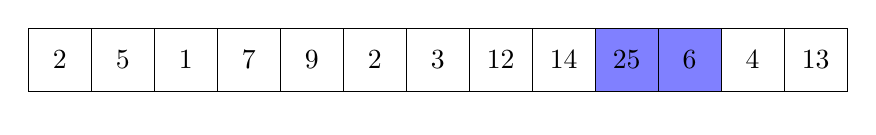
\begin{tikzpicture}
  \filldraw[fill=white!0, draw=none] (0cm,0cm) rectangle (10.4cm, -1cm);
  \filldraw[fill=white] (0cm,-0.8cm) rectangle (0.8cm,0cm);
  \node at (0.4cm,-0.4cm) {2};
  \filldraw[fill=white] (0.8cm,-0.8cm) rectangle (1.6cm,0cm);
  \node at (1.2000000000000002cm,-0.4cm) {5};
  \filldraw[fill=white] (1.6cm,-0.8cm) rectangle (2.4000000000000004cm,0cm);
  \node at (2cm,-0.4cm) {1};
  \filldraw[fill=white] (2.4000000000000004cm,-0.8cm) rectangle (3.2cm,0cm);
  \node at (2.8000000000000003cm,-0.4cm) {7};
  \filldraw[fill=white] (3.2cm,-0.8cm) rectangle (4cm,0cm);
  \node at (3.6cm,-0.4cm) {9};
  \filldraw[fill=white] (4cm,-0.8cm) rectangle (4.8cm,0cm);
  \node at (4.4cm,-0.4cm) {2};
  \filldraw[fill=white] (4.800000000000001cm,-0.8cm) rectangle (5.6000000000000005cm,0cm);
  \node at (5.200000000000001cm,-0.4cm) {3};
  \filldraw[fill=white] (5.6000000000000005cm,-0.8cm) rectangle (6.4cm,0cm);
  \node at (6.000000000000001cm,-0.4cm) {12};
  \filldraw[fill=white] (6.4cm,-0.8cm) rectangle (7.2cm,0cm);
  \node at (6.800000000000001cm,-0.4cm) {14};
  \filldraw[fill=blue!50] (7.2cm,-0.8cm) rectangle (8cm,0cm);
  \node at (7.6000000000000005cm,-0.4cm) {25};
  \filldraw[fill=blue!50] (8cm,-0.8cm) rectangle (8.8cm,0cm);
  \node at (8.4cm,-0.4cm) {6};
  \filldraw[fill=white] (8.8cm,-0.8cm) rectangle (9.600000000000001cm,0cm);
  \node at (9.200000000000001cm,-0.4cm) {4};
  \filldraw[fill=white] (9.600000000000001cm,-0.8cm) rectangle (10.400000000000002cm,0cm);
  \node at (10.000000000000002cm,-0.4cm) {13};
\end{tikzpicture}
\end{center}
\newpage
% --- Frame 17 ---
\begin{center}\LARGE\textbf{Algorithm}\\[6mm]\end{center}
\begin{center}
\begin{flushleft}\textbf{Log}\\[1.75mm]\end{flushleft}

\begin{tikzpicture}
  \filldraw[fill=white!0, draw=none] (0,0) rectangle (10cm, -0.25cm);
  \node[anchor=north, align=center, text=black] at (5cm,0) {\texttt{Swapping cells at index 9 and 10}};
\end{tikzpicture}
\end{center}
\noindent\rule{\linewidth}{0.3pt}
\begin{center}
\begin{flushleft}\textbf{Array}\\[1.75mm]\end{flushleft}
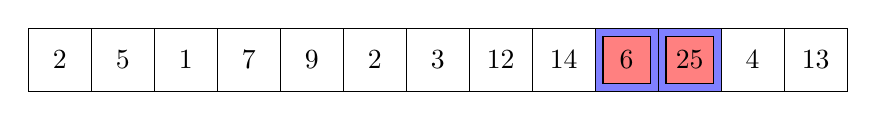
\begin{tikzpicture}
  \filldraw[fill=white!0, draw=none] (0cm,0cm) rectangle (10.4cm, -1cm);
  \filldraw[fill=white] (0cm,-0.8cm) rectangle (0.8cm,0cm);
  \node at (0.4cm,-0.4cm) {2};
  \filldraw[fill=white] (0.8cm,-0.8cm) rectangle (1.6cm,0cm);
  \node at (1.2000000000000002cm,-0.4cm) {5};
  \filldraw[fill=white] (1.6cm,-0.8cm) rectangle (2.4000000000000004cm,0cm);
  \node at (2cm,-0.4cm) {1};
  \filldraw[fill=white] (2.4000000000000004cm,-0.8cm) rectangle (3.2cm,0cm);
  \node at (2.8000000000000003cm,-0.4cm) {7};
  \filldraw[fill=white] (3.2cm,-0.8cm) rectangle (4cm,0cm);
  \node at (3.6cm,-0.4cm) {9};
  \filldraw[fill=white] (4cm,-0.8cm) rectangle (4.8cm,0cm);
  \node at (4.4cm,-0.4cm) {2};
  \filldraw[fill=white] (4.800000000000001cm,-0.8cm) rectangle (5.6000000000000005cm,0cm);
  \node at (5.200000000000001cm,-0.4cm) {3};
  \filldraw[fill=white] (5.6000000000000005cm,-0.8cm) rectangle (6.4cm,0cm);
  \node at (6.000000000000001cm,-0.4cm) {12};
  \filldraw[fill=white] (6.4cm,-0.8cm) rectangle (7.2cm,0cm);
  \node at (6.800000000000001cm,-0.4cm) {14};
  \filldraw[fill=blue!50] (7.2cm,-0.8cm) rectangle (8cm,0cm);
  \filldraw[fill=red!50] (7.3cm,-0.7000000000000001cm) rectangle (7.9cm,-0.1cm);
  \node at (7.6000000000000005cm,-0.4cm) {6};
  \filldraw[fill=blue!50] (8cm,-0.8cm) rectangle (8.8cm,0cm);
  \filldraw[fill=red!50] (8.1cm,-0.7000000000000001cm) rectangle (8.700000000000001cm,-0.1cm);
  \node at (8.4cm,-0.4cm) {25};
  \filldraw[fill=white] (8.8cm,-0.8cm) rectangle (9.600000000000001cm,0cm);
  \node at (9.200000000000001cm,-0.4cm) {4};
  \filldraw[fill=white] (9.600000000000001cm,-0.8cm) rectangle (10.400000000000002cm,0cm);
  \node at (10.000000000000002cm,-0.4cm) {13};
\end{tikzpicture}
\end{center}
\newpage
% --- Frame 18 ---
\begin{center}\LARGE\textbf{Algorithm}\\[6mm]\end{center}
\begin{center}
\begin{flushleft}\textbf{Log}\\[1.75mm]\end{flushleft}

\begin{tikzpicture}
  \filldraw[fill=white!0, draw=none] (0,0) rectangle (10cm, -0.25cm);
  \node[anchor=north, align=center, text=black] at (5cm,0) {\texttt{Comparing cells at index 10 and 11}};
\end{tikzpicture}
\end{center}
\noindent\rule{\linewidth}{0.3pt}
\begin{center}
\begin{flushleft}\textbf{Array}\\[1.75mm]\end{flushleft}
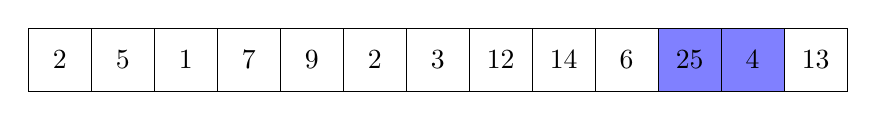
\begin{tikzpicture}
  \filldraw[fill=white!0, draw=none] (0cm,0cm) rectangle (10.4cm, -1cm);
  \filldraw[fill=white] (0cm,-0.8cm) rectangle (0.8cm,0cm);
  \node at (0.4cm,-0.4cm) {2};
  \filldraw[fill=white] (0.8cm,-0.8cm) rectangle (1.6cm,0cm);
  \node at (1.2000000000000002cm,-0.4cm) {5};
  \filldraw[fill=white] (1.6cm,-0.8cm) rectangle (2.4000000000000004cm,0cm);
  \node at (2cm,-0.4cm) {1};
  \filldraw[fill=white] (2.4000000000000004cm,-0.8cm) rectangle (3.2cm,0cm);
  \node at (2.8000000000000003cm,-0.4cm) {7};
  \filldraw[fill=white] (3.2cm,-0.8cm) rectangle (4cm,0cm);
  \node at (3.6cm,-0.4cm) {9};
  \filldraw[fill=white] (4cm,-0.8cm) rectangle (4.8cm,0cm);
  \node at (4.4cm,-0.4cm) {2};
  \filldraw[fill=white] (4.800000000000001cm,-0.8cm) rectangle (5.6000000000000005cm,0cm);
  \node at (5.200000000000001cm,-0.4cm) {3};
  \filldraw[fill=white] (5.6000000000000005cm,-0.8cm) rectangle (6.4cm,0cm);
  \node at (6.000000000000001cm,-0.4cm) {12};
  \filldraw[fill=white] (6.4cm,-0.8cm) rectangle (7.2cm,0cm);
  \node at (6.800000000000001cm,-0.4cm) {14};
  \filldraw[fill=white] (7.2cm,-0.8cm) rectangle (8cm,0cm);
  \node at (7.6000000000000005cm,-0.4cm) {6};
  \filldraw[fill=blue!50] (8cm,-0.8cm) rectangle (8.8cm,0cm);
  \node at (8.4cm,-0.4cm) {25};
  \filldraw[fill=blue!50] (8.8cm,-0.8cm) rectangle (9.600000000000001cm,0cm);
  \node at (9.200000000000001cm,-0.4cm) {4};
  \filldraw[fill=white] (9.600000000000001cm,-0.8cm) rectangle (10.400000000000002cm,0cm);
  \node at (10.000000000000002cm,-0.4cm) {13};
\end{tikzpicture}
\end{center}
\newpage
% --- Frame 19 ---
\begin{center}\LARGE\textbf{Algorithm}\\[6mm]\end{center}
\begin{center}
\begin{flushleft}\textbf{Log}\\[1.75mm]\end{flushleft}

\begin{tikzpicture}
  \filldraw[fill=white!0, draw=none] (0,0) rectangle (10cm, -0.25cm);
  \node[anchor=north, align=center, text=black] at (5cm,0) {\texttt{Swapping cells at index 10 and 11}};
\end{tikzpicture}
\end{center}
\noindent\rule{\linewidth}{0.3pt}
\begin{center}
\begin{flushleft}\textbf{Array}\\[1.75mm]\end{flushleft}
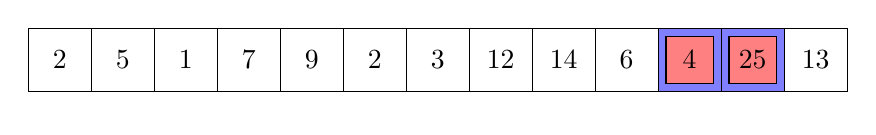
\begin{tikzpicture}
  \filldraw[fill=white!0, draw=none] (0cm,0cm) rectangle (10.4cm, -1cm);
  \filldraw[fill=white] (0cm,-0.8cm) rectangle (0.8cm,0cm);
  \node at (0.4cm,-0.4cm) {2};
  \filldraw[fill=white] (0.8cm,-0.8cm) rectangle (1.6cm,0cm);
  \node at (1.2000000000000002cm,-0.4cm) {5};
  \filldraw[fill=white] (1.6cm,-0.8cm) rectangle (2.4000000000000004cm,0cm);
  \node at (2cm,-0.4cm) {1};
  \filldraw[fill=white] (2.4000000000000004cm,-0.8cm) rectangle (3.2cm,0cm);
  \node at (2.8000000000000003cm,-0.4cm) {7};
  \filldraw[fill=white] (3.2cm,-0.8cm) rectangle (4cm,0cm);
  \node at (3.6cm,-0.4cm) {9};
  \filldraw[fill=white] (4cm,-0.8cm) rectangle (4.8cm,0cm);
  \node at (4.4cm,-0.4cm) {2};
  \filldraw[fill=white] (4.800000000000001cm,-0.8cm) rectangle (5.6000000000000005cm,0cm);
  \node at (5.200000000000001cm,-0.4cm) {3};
  \filldraw[fill=white] (5.6000000000000005cm,-0.8cm) rectangle (6.4cm,0cm);
  \node at (6.000000000000001cm,-0.4cm) {12};
  \filldraw[fill=white] (6.4cm,-0.8cm) rectangle (7.2cm,0cm);
  \node at (6.800000000000001cm,-0.4cm) {14};
  \filldraw[fill=white] (7.2cm,-0.8cm) rectangle (8cm,0cm);
  \node at (7.6000000000000005cm,-0.4cm) {6};
  \filldraw[fill=blue!50] (8cm,-0.8cm) rectangle (8.8cm,0cm);
  \filldraw[fill=red!50] (8.1cm,-0.7000000000000001cm) rectangle (8.700000000000001cm,-0.1cm);
  \node at (8.4cm,-0.4cm) {4};
  \filldraw[fill=blue!50] (8.8cm,-0.8cm) rectangle (9.600000000000001cm,0cm);
  \filldraw[fill=red!50] (8.9cm,-0.7000000000000001cm) rectangle (9.500000000000002cm,-0.1cm);
  \node at (9.200000000000001cm,-0.4cm) {25};
  \filldraw[fill=white] (9.600000000000001cm,-0.8cm) rectangle (10.400000000000002cm,0cm);
  \node at (10.000000000000002cm,-0.4cm) {13};
\end{tikzpicture}
\end{center}
\newpage
% --- Frame 20 ---
\begin{center}\LARGE\textbf{Algorithm}\\[6mm]\end{center}
\begin{center}
\begin{flushleft}\textbf{Log}\\[1.75mm]\end{flushleft}

\begin{tikzpicture}
  \filldraw[fill=white!0, draw=none] (0,0) rectangle (10cm, -0.25cm);
  \node[anchor=north, align=center, text=black] at (5cm,0) {\texttt{Comparing cells at index 11 and 12}};
\end{tikzpicture}
\end{center}
\noindent\rule{\linewidth}{0.3pt}
\begin{center}
\begin{flushleft}\textbf{Array}\\[1.75mm]\end{flushleft}
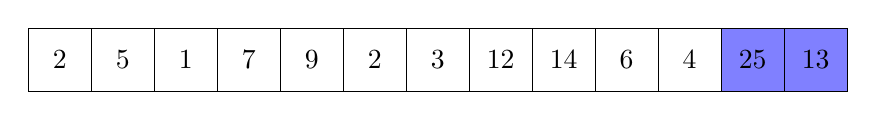
\begin{tikzpicture}
  \filldraw[fill=white!0, draw=none] (0cm,0cm) rectangle (10.4cm, -1cm);
  \filldraw[fill=white] (0cm,-0.8cm) rectangle (0.8cm,0cm);
  \node at (0.4cm,-0.4cm) {2};
  \filldraw[fill=white] (0.8cm,-0.8cm) rectangle (1.6cm,0cm);
  \node at (1.2000000000000002cm,-0.4cm) {5};
  \filldraw[fill=white] (1.6cm,-0.8cm) rectangle (2.4000000000000004cm,0cm);
  \node at (2cm,-0.4cm) {1};
  \filldraw[fill=white] (2.4000000000000004cm,-0.8cm) rectangle (3.2cm,0cm);
  \node at (2.8000000000000003cm,-0.4cm) {7};
  \filldraw[fill=white] (3.2cm,-0.8cm) rectangle (4cm,0cm);
  \node at (3.6cm,-0.4cm) {9};
  \filldraw[fill=white] (4cm,-0.8cm) rectangle (4.8cm,0cm);
  \node at (4.4cm,-0.4cm) {2};
  \filldraw[fill=white] (4.800000000000001cm,-0.8cm) rectangle (5.6000000000000005cm,0cm);
  \node at (5.200000000000001cm,-0.4cm) {3};
  \filldraw[fill=white] (5.6000000000000005cm,-0.8cm) rectangle (6.4cm,0cm);
  \node at (6.000000000000001cm,-0.4cm) {12};
  \filldraw[fill=white] (6.4cm,-0.8cm) rectangle (7.2cm,0cm);
  \node at (6.800000000000001cm,-0.4cm) {14};
  \filldraw[fill=white] (7.2cm,-0.8cm) rectangle (8cm,0cm);
  \node at (7.6000000000000005cm,-0.4cm) {6};
  \filldraw[fill=white] (8cm,-0.8cm) rectangle (8.8cm,0cm);
  \node at (8.4cm,-0.4cm) {4};
  \filldraw[fill=blue!50] (8.8cm,-0.8cm) rectangle (9.600000000000001cm,0cm);
  \node at (9.200000000000001cm,-0.4cm) {25};
  \filldraw[fill=blue!50] (9.600000000000001cm,-0.8cm) rectangle (10.400000000000002cm,0cm);
  \node at (10.000000000000002cm,-0.4cm) {13};
\end{tikzpicture}
\end{center}
\newpage
% --- Frame 21 ---
\begin{center}\LARGE\textbf{Algorithm}\\[6mm]\end{center}
\begin{center}
\begin{flushleft}\textbf{Log}\\[1.75mm]\end{flushleft}

\begin{tikzpicture}
  \filldraw[fill=white!0, draw=none] (0,0) rectangle (10cm, -0.25cm);
  \node[anchor=north, align=center, text=black] at (5cm,0) {\texttt{Swapping cells at index 11 and 12}};
\end{tikzpicture}
\end{center}
\noindent\rule{\linewidth}{0.3pt}
\begin{center}
\begin{flushleft}\textbf{Array}\\[1.75mm]\end{flushleft}
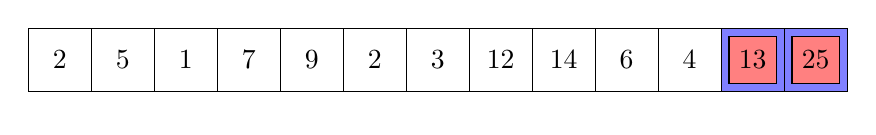
\begin{tikzpicture}
  \filldraw[fill=white!0, draw=none] (0cm,0cm) rectangle (10.4cm, -1cm);
  \filldraw[fill=white] (0cm,-0.8cm) rectangle (0.8cm,0cm);
  \node at (0.4cm,-0.4cm) {2};
  \filldraw[fill=white] (0.8cm,-0.8cm) rectangle (1.6cm,0cm);
  \node at (1.2000000000000002cm,-0.4cm) {5};
  \filldraw[fill=white] (1.6cm,-0.8cm) rectangle (2.4000000000000004cm,0cm);
  \node at (2cm,-0.4cm) {1};
  \filldraw[fill=white] (2.4000000000000004cm,-0.8cm) rectangle (3.2cm,0cm);
  \node at (2.8000000000000003cm,-0.4cm) {7};
  \filldraw[fill=white] (3.2cm,-0.8cm) rectangle (4cm,0cm);
  \node at (3.6cm,-0.4cm) {9};
  \filldraw[fill=white] (4cm,-0.8cm) rectangle (4.8cm,0cm);
  \node at (4.4cm,-0.4cm) {2};
  \filldraw[fill=white] (4.800000000000001cm,-0.8cm) rectangle (5.6000000000000005cm,0cm);
  \node at (5.200000000000001cm,-0.4cm) {3};
  \filldraw[fill=white] (5.6000000000000005cm,-0.8cm) rectangle (6.4cm,0cm);
  \node at (6.000000000000001cm,-0.4cm) {12};
  \filldraw[fill=white] (6.4cm,-0.8cm) rectangle (7.2cm,0cm);
  \node at (6.800000000000001cm,-0.4cm) {14};
  \filldraw[fill=white] (7.2cm,-0.8cm) rectangle (8cm,0cm);
  \node at (7.6000000000000005cm,-0.4cm) {6};
  \filldraw[fill=white] (8cm,-0.8cm) rectangle (8.8cm,0cm);
  \node at (8.4cm,-0.4cm) {4};
  \filldraw[fill=blue!50] (8.8cm,-0.8cm) rectangle (9.600000000000001cm,0cm);
  \filldraw[fill=red!50] (8.9cm,-0.7000000000000001cm) rectangle (9.500000000000002cm,-0.1cm);
  \node at (9.200000000000001cm,-0.4cm) {13};
  \filldraw[fill=blue!50] (9.600000000000001cm,-0.8cm) rectangle (10.400000000000002cm,0cm);
  \filldraw[fill=red!50] (9.700000000000001cm,-0.7000000000000001cm) rectangle (10.300000000000002cm,-0.1cm);
  \node at (10.000000000000002cm,-0.4cm) {25};
\end{tikzpicture}
\end{center}
\newpage
% --- Frame 22 ---
\begin{center}\LARGE\textbf{Algorithm}\\[6mm]\end{center}
\begin{center}
\begin{flushleft}\textbf{Log}\\[1.75mm]\end{flushleft}

\begin{tikzpicture}
  \filldraw[fill=white!0, draw=none] (0,0) rectangle (10cm, -0.25cm);
  \node[anchor=north, align=center, text=black] at (5cm,0) {\texttt{Comparing cells at index 0 and 1}};
\end{tikzpicture}
\end{center}
\noindent\rule{\linewidth}{0.3pt}
\begin{center}
\begin{flushleft}\textbf{Array}\\[1.75mm]\end{flushleft}
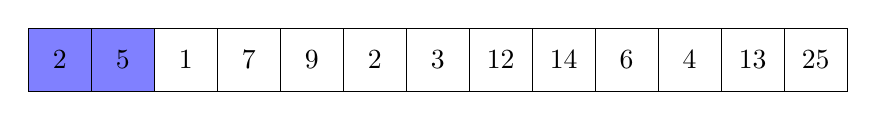
\begin{tikzpicture}
  \filldraw[fill=white!0, draw=none] (0cm,0cm) rectangle (10.4cm, -1cm);
  \filldraw[fill=blue!50] (0cm,-0.8cm) rectangle (0.8cm,0cm);
  \node at (0.4cm,-0.4cm) {2};
  \filldraw[fill=blue!50] (0.8cm,-0.8cm) rectangle (1.6cm,0cm);
  \node at (1.2000000000000002cm,-0.4cm) {5};
  \filldraw[fill=white] (1.6cm,-0.8cm) rectangle (2.4000000000000004cm,0cm);
  \node at (2cm,-0.4cm) {1};
  \filldraw[fill=white] (2.4000000000000004cm,-0.8cm) rectangle (3.2cm,0cm);
  \node at (2.8000000000000003cm,-0.4cm) {7};
  \filldraw[fill=white] (3.2cm,-0.8cm) rectangle (4cm,0cm);
  \node at (3.6cm,-0.4cm) {9};
  \filldraw[fill=white] (4cm,-0.8cm) rectangle (4.8cm,0cm);
  \node at (4.4cm,-0.4cm) {2};
  \filldraw[fill=white] (4.800000000000001cm,-0.8cm) rectangle (5.6000000000000005cm,0cm);
  \node at (5.200000000000001cm,-0.4cm) {3};
  \filldraw[fill=white] (5.6000000000000005cm,-0.8cm) rectangle (6.4cm,0cm);
  \node at (6.000000000000001cm,-0.4cm) {12};
  \filldraw[fill=white] (6.4cm,-0.8cm) rectangle (7.2cm,0cm);
  \node at (6.800000000000001cm,-0.4cm) {14};
  \filldraw[fill=white] (7.2cm,-0.8cm) rectangle (8cm,0cm);
  \node at (7.6000000000000005cm,-0.4cm) {6};
  \filldraw[fill=white] (8cm,-0.8cm) rectangle (8.8cm,0cm);
  \node at (8.4cm,-0.4cm) {4};
  \filldraw[fill=white] (8.8cm,-0.8cm) rectangle (9.600000000000001cm,0cm);
  \node at (9.200000000000001cm,-0.4cm) {13};
  \filldraw[fill=white] (9.600000000000001cm,-0.8cm) rectangle (10.400000000000002cm,0cm);
  \node at (10.000000000000002cm,-0.4cm) {25};
\end{tikzpicture}
\end{center}
\newpage
% --- Frame 23 ---
\begin{center}\LARGE\textbf{Algorithm}\\[6mm]\end{center}
\begin{center}
\begin{flushleft}\textbf{Log}\\[1.75mm]\end{flushleft}

\begin{tikzpicture}
  \filldraw[fill=white!0, draw=none] (0,0) rectangle (10cm, -0.25cm);
  \node[anchor=north, align=center, text=black] at (5cm,0) {\texttt{Comparing cells at index 1 and 2}};
\end{tikzpicture}
\end{center}
\noindent\rule{\linewidth}{0.3pt}
\begin{center}
\begin{flushleft}\textbf{Array}\\[1.75mm]\end{flushleft}
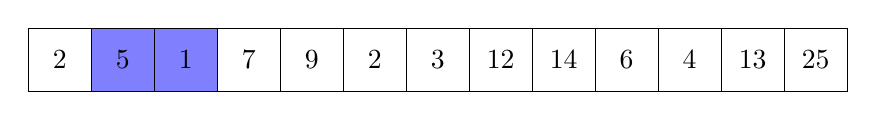
\begin{tikzpicture}
  \filldraw[fill=white!0, draw=none] (0cm,0cm) rectangle (10.4cm, -1cm);
  \filldraw[fill=white] (0cm,-0.8cm) rectangle (0.8cm,0cm);
  \node at (0.4cm,-0.4cm) {2};
  \filldraw[fill=blue!50] (0.8cm,-0.8cm) rectangle (1.6cm,0cm);
  \node at (1.2000000000000002cm,-0.4cm) {5};
  \filldraw[fill=blue!50] (1.6cm,-0.8cm) rectangle (2.4000000000000004cm,0cm);
  \node at (2cm,-0.4cm) {1};
  \filldraw[fill=white] (2.4000000000000004cm,-0.8cm) rectangle (3.2cm,0cm);
  \node at (2.8000000000000003cm,-0.4cm) {7};
  \filldraw[fill=white] (3.2cm,-0.8cm) rectangle (4cm,0cm);
  \node at (3.6cm,-0.4cm) {9};
  \filldraw[fill=white] (4cm,-0.8cm) rectangle (4.8cm,0cm);
  \node at (4.4cm,-0.4cm) {2};
  \filldraw[fill=white] (4.800000000000001cm,-0.8cm) rectangle (5.6000000000000005cm,0cm);
  \node at (5.200000000000001cm,-0.4cm) {3};
  \filldraw[fill=white] (5.6000000000000005cm,-0.8cm) rectangle (6.4cm,0cm);
  \node at (6.000000000000001cm,-0.4cm) {12};
  \filldraw[fill=white] (6.4cm,-0.8cm) rectangle (7.2cm,0cm);
  \node at (6.800000000000001cm,-0.4cm) {14};
  \filldraw[fill=white] (7.2cm,-0.8cm) rectangle (8cm,0cm);
  \node at (7.6000000000000005cm,-0.4cm) {6};
  \filldraw[fill=white] (8cm,-0.8cm) rectangle (8.8cm,0cm);
  \node at (8.4cm,-0.4cm) {4};
  \filldraw[fill=white] (8.8cm,-0.8cm) rectangle (9.600000000000001cm,0cm);
  \node at (9.200000000000001cm,-0.4cm) {13};
  \filldraw[fill=white] (9.600000000000001cm,-0.8cm) rectangle (10.400000000000002cm,0cm);
  \node at (10.000000000000002cm,-0.4cm) {25};
\end{tikzpicture}
\end{center}
\newpage
% --- Frame 24 ---
\begin{center}\LARGE\textbf{Algorithm}\\[6mm]\end{center}
\begin{center}
\begin{flushleft}\textbf{Log}\\[1.75mm]\end{flushleft}

\begin{tikzpicture}
  \filldraw[fill=white!0, draw=none] (0,0) rectangle (10cm, -0.25cm);
  \node[anchor=north, align=center, text=black] at (5cm,0) {\texttt{Swapping cells at index 1 and 2}};
\end{tikzpicture}
\end{center}
\noindent\rule{\linewidth}{0.3pt}
\begin{center}
\begin{flushleft}\textbf{Array}\\[1.75mm]\end{flushleft}
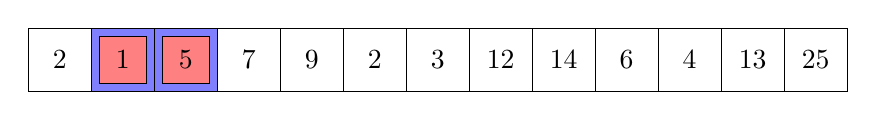
\begin{tikzpicture}
  \filldraw[fill=white!0, draw=none] (0cm,0cm) rectangle (10.4cm, -1cm);
  \filldraw[fill=white] (0cm,-0.8cm) rectangle (0.8cm,0cm);
  \node at (0.4cm,-0.4cm) {2};
  \filldraw[fill=blue!50] (0.8cm,-0.8cm) rectangle (1.6cm,0cm);
  \filldraw[fill=red!50] (0.9cm,-0.7000000000000001cm) rectangle (1.5cm,-0.1cm);
  \node at (1.2000000000000002cm,-0.4cm) {1};
  \filldraw[fill=blue!50] (1.6cm,-0.8cm) rectangle (2.4000000000000004cm,0cm);
  \filldraw[fill=red!50] (1.7000000000000002cm,-0.7000000000000001cm) rectangle (2.3000000000000003cm,-0.1cm);
  \node at (2cm,-0.4cm) {5};
  \filldraw[fill=white] (2.4000000000000004cm,-0.8cm) rectangle (3.2cm,0cm);
  \node at (2.8000000000000003cm,-0.4cm) {7};
  \filldraw[fill=white] (3.2cm,-0.8cm) rectangle (4cm,0cm);
  \node at (3.6cm,-0.4cm) {9};
  \filldraw[fill=white] (4cm,-0.8cm) rectangle (4.8cm,0cm);
  \node at (4.4cm,-0.4cm) {2};
  \filldraw[fill=white] (4.800000000000001cm,-0.8cm) rectangle (5.6000000000000005cm,0cm);
  \node at (5.200000000000001cm,-0.4cm) {3};
  \filldraw[fill=white] (5.6000000000000005cm,-0.8cm) rectangle (6.4cm,0cm);
  \node at (6.000000000000001cm,-0.4cm) {12};
  \filldraw[fill=white] (6.4cm,-0.8cm) rectangle (7.2cm,0cm);
  \node at (6.800000000000001cm,-0.4cm) {14};
  \filldraw[fill=white] (7.2cm,-0.8cm) rectangle (8cm,0cm);
  \node at (7.6000000000000005cm,-0.4cm) {6};
  \filldraw[fill=white] (8cm,-0.8cm) rectangle (8.8cm,0cm);
  \node at (8.4cm,-0.4cm) {4};
  \filldraw[fill=white] (8.8cm,-0.8cm) rectangle (9.600000000000001cm,0cm);
  \node at (9.200000000000001cm,-0.4cm) {13};
  \filldraw[fill=white] (9.600000000000001cm,-0.8cm) rectangle (10.400000000000002cm,0cm);
  \node at (10.000000000000002cm,-0.4cm) {25};
\end{tikzpicture}
\end{center}
\newpage
% --- Frame 25 ---
\begin{center}\LARGE\textbf{Algorithm}\\[6mm]\end{center}
\begin{center}
\begin{flushleft}\textbf{Log}\\[1.75mm]\end{flushleft}
\begin{tikzpicture}
  \filldraw[fill=white!0, draw=none] (0,0) rectangle (10cm, -0.25cm);
  \node[anchor=north, align=center, text=black] at (5cm,0) {\texttt{Comparing cells at index 2 and 3}};
\end{tikzpicture}
\end{center}
\noindent\rule{\linewidth}{0.3pt}
\begin{center}
\begin{flushleft}\textbf{Array}\\[1.75mm]\end{flushleft}
\begin{tikzpicture}
  \filldraw[fill=white!0, draw=none] (0cm,0cm) rectangle (10.4cm, -1cm);
  \filldraw[fill=white] (0cm,-0.8cm) rectangle (0.8cm,0cm);
  \node at (0.4cm,-0.4cm) {2};
  \filldraw[fill=white] (0.8cm,-0.8cm) rectangle (1.6cm,0cm);
  \node at (1.2000000000000002cm,-0.4cm) {1};
  \filldraw[fill=blue!50] (1.6cm,-0.8cm) rectangle (2.4000000000000004cm,0cm);
  \node at (2cm,-0.4cm) {5};
  \filldraw[fill=blue!50] (2.4000000000000004cm,-0.8cm) rectangle (3.2cm,0cm);
  \node at (2.8000000000000003cm,-0.4cm) {7};
  \filldraw[fill=white] (3.2cm,-0.8cm) rectangle (4cm,0cm);
  \node at (3.6cm,-0.4cm) {9};
  \filldraw[fill=white] (4cm,-0.8cm) rectangle (4.8cm,0cm);
  \node at (4.4cm,-0.4cm) {2};
  \filldraw[fill=white] (4.800000000000001cm,-0.8cm) rectangle (5.6000000000000005cm,0cm);
  \node at (5.200000000000001cm,-0.4cm) {3};
  \filldraw[fill=white] (5.6000000000000005cm,-0.8cm) rectangle (6.4cm,0cm);
  \node at (6.000000000000001cm,-0.4cm) {12};
  \filldraw[fill=white] (6.4cm,-0.8cm) rectangle (7.2cm,0cm);
  \node at (6.800000000000001cm,-0.4cm) {14};
  \filldraw[fill=white] (7.2cm,-0.8cm) rectangle (8cm,0cm);
  \node at (7.6000000000000005cm,-0.4cm) {6};
  \filldraw[fill=white] (8cm,-0.8cm) rectangle (8.8cm,0cm);
  \node at (8.4cm,-0.4cm) {4};
  \filldraw[fill=white] (8.8cm,-0.8cm) rectangle (9.600000000000001cm,0cm);
  \node at (9.200000000000001cm,-0.4cm) {13};
  \filldraw[fill=white] (9.600000000000001cm,-0.8cm) rectangle (10.400000000000002cm,0cm);
  \node at (10.000000000000002cm,-0.4cm) {25};
\end{tikzpicture}
\end{center}
\newpage
% --- Frame 26 ---
\begin{center}\LARGE\textbf{Algorithm}\\[6mm]\end{center}
\begin{center}
\begin{flushleft}\textbf{Log}\\[1.75mm]\end{flushleft}
\begin{tikzpicture}
  \filldraw[fill=white!0, draw=none] (0,0) rectangle (10cm, -0.25cm);
  \node[anchor=north, align=center, text=black] at (5cm,0) {\texttt{Comparing cells at index 3 and 4}};
\end{tikzpicture}
\end{center}
\noindent\rule{\linewidth}{0.3pt}
\begin{center}
\begin{flushleft}\textbf{Array}\\[1.75mm]\end{flushleft}
\begin{tikzpicture}
  \filldraw[fill=white!0, draw=none] (0cm,0cm) rectangle (10.4cm, -1cm);
  \filldraw[fill=white] (0cm,-0.8cm) rectangle (0.8cm,0cm);
  \node at (0.4cm,-0.4cm) {2};
  \filldraw[fill=white] (0.8cm,-0.8cm) rectangle (1.6cm,0cm);
  \node at (1.2000000000000002cm,-0.4cm) {1};
  \filldraw[fill=white] (1.6cm,-0.8cm) rectangle (2.4000000000000004cm,0cm);
  \node at (2cm,-0.4cm) {5};
  \filldraw[fill=blue!50] (2.4000000000000004cm,-0.8cm) rectangle (3.2cm,0cm);
  \node at (2.8000000000000003cm,-0.4cm) {7};
  \filldraw[fill=blue!50] (3.2cm,-0.8cm) rectangle (4cm,0cm);
  \node at (3.6cm,-0.4cm) {9};
  \filldraw[fill=white] (4cm,-0.8cm) rectangle (4.8cm,0cm);
  \node at (4.4cm,-0.4cm) {2};
  \filldraw[fill=white] (4.800000000000001cm,-0.8cm) rectangle (5.6000000000000005cm,0cm);
  \node at (5.200000000000001cm,-0.4cm) {3};
  \filldraw[fill=white] (5.6000000000000005cm,-0.8cm) rectangle (6.4cm,0cm);
  \node at (6.000000000000001cm,-0.4cm) {12};
  \filldraw[fill=white] (6.4cm,-0.8cm) rectangle (7.2cm,0cm);
  \node at (6.800000000000001cm,-0.4cm) {14};
  \filldraw[fill=white] (7.2cm,-0.8cm) rectangle (8cm,0cm);
  \node at (7.6000000000000005cm,-0.4cm) {6};
  \filldraw[fill=white] (8cm,-0.8cm) rectangle (8.8cm,0cm);
  \node at (8.4cm,-0.4cm) {4};
  \filldraw[fill=white] (8.8cm,-0.8cm) rectangle (9.600000000000001cm,0cm);
  \node at (9.200000000000001cm,-0.4cm) {13};
  \filldraw[fill=white] (9.600000000000001cm,-0.8cm) rectangle (10.400000000000002cm,0cm);
  \node at (10.000000000000002cm,-0.4cm) {25};
\end{tikzpicture}
\end{center}
\newpage
% --- Frame 27 ---
\begin{center}\LARGE\textbf{Algorithm}\\[6mm]\end{center}
\begin{center}
\begin{flushleft}\textbf{Log}\\[1.75mm]\end{flushleft}
\begin{tikzpicture}
  \filldraw[fill=white!0, draw=none] (0,0) rectangle (10cm, -0.25cm);
  \node[anchor=north, align=center, text=black] at (5cm,0) {\texttt{Comparing cells at index 4 and 5}};
\end{tikzpicture}
\end{center}
\noindent\rule{\linewidth}{0.3pt}
\begin{center}
\begin{flushleft}\textbf{Array}\\[1.75mm]\end{flushleft}
\begin{tikzpicture}
  \filldraw[fill=white!0, draw=none] (0cm,0cm) rectangle (10.4cm, -1cm);
  \filldraw[fill=white] (0cm,-0.8cm) rectangle (0.8cm,0cm);
  \node at (0.4cm,-0.4cm) {2};
  \filldraw[fill=white] (0.8cm,-0.8cm) rectangle (1.6cm,0cm);
  \node at (1.2000000000000002cm,-0.4cm) {1};
  \filldraw[fill=white] (1.6cm,-0.8cm) rectangle (2.4000000000000004cm,0cm);
  \node at (2cm,-0.4cm) {5};
  \filldraw[fill=white] (2.4000000000000004cm,-0.8cm) rectangle (3.2cm,0cm);
  \node at (2.8000000000000003cm,-0.4cm) {7};
  \filldraw[fill=blue!50] (3.2cm,-0.8cm) rectangle (4cm,0cm);
  \node at (3.6cm,-0.4cm) {9};
  \filldraw[fill=blue!50] (4cm,-0.8cm) rectangle (4.8cm,0cm);
  \node at (4.4cm,-0.4cm) {2};
  \filldraw[fill=white] (4.800000000000001cm,-0.8cm) rectangle (5.6000000000000005cm,0cm);
  \node at (5.200000000000001cm,-0.4cm) {3};
  \filldraw[fill=white] (5.6000000000000005cm,-0.8cm) rectangle (6.4cm,0cm);
  \node at (6.000000000000001cm,-0.4cm) {12};
  \filldraw[fill=white] (6.4cm,-0.8cm) rectangle (7.2cm,0cm);
  \node at (6.800000000000001cm,-0.4cm) {14};
  \filldraw[fill=white] (7.2cm,-0.8cm) rectangle (8cm,0cm);
  \node at (7.6000000000000005cm,-0.4cm) {6};
  \filldraw[fill=white] (8cm,-0.8cm) rectangle (8.8cm,0cm);
  \node at (8.4cm,-0.4cm) {4};
  \filldraw[fill=white] (8.8cm,-0.8cm) rectangle (9.600000000000001cm,0cm);
  \node at (9.200000000000001cm,-0.4cm) {13};
  \filldraw[fill=white] (9.600000000000001cm,-0.8cm) rectangle (10.400000000000002cm,0cm);
  \node at (10.000000000000002cm,-0.4cm) {25};
\end{tikzpicture}
\end{center}
\newpage
% --- Frame 28 ---
\begin{center}\LARGE\textbf{Algorithm}\\[6mm]\end{center}
\begin{center}
\begin{flushleft}\textbf{Log}\\[1.75mm]\end{flushleft}
\begin{tikzpicture}
  \filldraw[fill=white!0, draw=none] (0,0) rectangle (10cm, -0.25cm);
  \node[anchor=north, align=center, text=black] at (5cm,0) {\texttt{Swapping cells at index 4 and 5}};
\end{tikzpicture}
\end{center}
\noindent\rule{\linewidth}{0.3pt}
\begin{center}
\begin{flushleft}\textbf{Array}\\[1.75mm]\end{flushleft}
\begin{tikzpicture}
  \filldraw[fill=white!0, draw=none] (0cm,0cm) rectangle (10.4cm, -1cm);
  \filldraw[fill=white] (0cm,-0.8cm) rectangle (0.8cm,0cm);
  \node at (0.4cm,-0.4cm) {2};
  \filldraw[fill=white] (0.8cm,-0.8cm) rectangle (1.6cm,0cm);
  \node at (1.2000000000000002cm,-0.4cm) {1};
  \filldraw[fill=white] (1.6cm,-0.8cm) rectangle (2.4000000000000004cm,0cm);
  \node at (2cm,-0.4cm) {5};
  \filldraw[fill=white] (2.4000000000000004cm,-0.8cm) rectangle (3.2cm,0cm);
  \node at (2.8000000000000003cm,-0.4cm) {7};
  \filldraw[fill=blue!50] (3.2cm,-0.8cm) rectangle (4cm,0cm);
  \filldraw[fill=red!50] (3.3000000000000003cm,-0.7000000000000001cm) rectangle (3.9cm,-0.1cm);
  \node at (3.6cm,-0.4cm) {2};
  \filldraw[fill=blue!50] (4cm,-0.8cm) rectangle (4.8cm,0cm);
  \filldraw[fill=red!50] (4.1cm,-0.7000000000000001cm) rectangle (4.7cm,-0.1cm);
  \node at (4.4cm,-0.4cm) {9};
  \filldraw[fill=white] (4.800000000000001cm,-0.8cm) rectangle (5.6000000000000005cm,0cm);
  \node at (5.200000000000001cm,-0.4cm) {3};
  \filldraw[fill=white] (5.6000000000000005cm,-0.8cm) rectangle (6.4cm,0cm);
  \node at (6.000000000000001cm,-0.4cm) {12};
  \filldraw[fill=white] (6.4cm,-0.8cm) rectangle (7.2cm,0cm);
  \node at (6.800000000000001cm,-0.4cm) {14};
  \filldraw[fill=white] (7.2cm,-0.8cm) rectangle (8cm,0cm);
  \node at (7.6000000000000005cm,-0.4cm) {6};
  \filldraw[fill=white] (8cm,-0.8cm) rectangle (8.8cm,0cm);
  \node at (8.4cm,-0.4cm) {4};
  \filldraw[fill=white] (8.8cm,-0.8cm) rectangle (9.600000000000001cm,0cm);
  \node at (9.200000000000001cm,-0.4cm) {13};
  \filldraw[fill=white] (9.600000000000001cm,-0.8cm) rectangle (10.400000000000002cm,0cm);
  \node at (10.000000000000002cm,-0.4cm) {25};
\end{tikzpicture}
\end{center}
\newpage
% --- Frame 29 ---
\begin{center}\LARGE\textbf{Algorithm}\\[6mm]\end{center}
\begin{center}
\begin{flushleft}\textbf{Log}\\[1.75mm]\end{flushleft}
\begin{tikzpicture}
  \filldraw[fill=white!0, draw=none] (0,0) rectangle (10cm, -0.25cm);
  \node[anchor=north, align=center, text=black] at (5cm,0) {\texttt{Comparing cells at index 5 and 6}};
\end{tikzpicture}
\end{center}
\noindent\rule{\linewidth}{0.3pt}
\begin{center}
\begin{flushleft}\textbf{Array}\\[1.75mm]\end{flushleft}
\begin{tikzpicture}
  \filldraw[fill=white!0, draw=none] (0cm,0cm) rectangle (10.4cm, -1cm);
  \filldraw[fill=white] (0cm,-0.8cm) rectangle (0.8cm,0cm);
  \node at (0.4cm,-0.4cm) {2};
  \filldraw[fill=white] (0.8cm,-0.8cm) rectangle (1.6cm,0cm);
  \node at (1.2000000000000002cm,-0.4cm) {1};
  \filldraw[fill=white] (1.6cm,-0.8cm) rectangle (2.4000000000000004cm,0cm);
  \node at (2cm,-0.4cm) {5};
  \filldraw[fill=white] (2.4000000000000004cm,-0.8cm) rectangle (3.2cm,0cm);
  \node at (2.8000000000000003cm,-0.4cm) {7};
  \filldraw[fill=white] (3.2cm,-0.8cm) rectangle (4cm,0cm);
  \node at (3.6cm,-0.4cm) {2};
  \filldraw[fill=blue!50] (4cm,-0.8cm) rectangle (4.8cm,0cm);
  \node at (4.4cm,-0.4cm) {9};
  \filldraw[fill=blue!50] (4.800000000000001cm,-0.8cm) rectangle (5.6000000000000005cm,0cm);
  \node at (5.200000000000001cm,-0.4cm) {3};
  \filldraw[fill=white] (5.6000000000000005cm,-0.8cm) rectangle (6.4cm,0cm);
  \node at (6.000000000000001cm,-0.4cm) {12};
  \filldraw[fill=white] (6.4cm,-0.8cm) rectangle (7.2cm,0cm);
  \node at (6.800000000000001cm,-0.4cm) {14};
  \filldraw[fill=white] (7.2cm,-0.8cm) rectangle (8cm,0cm);
  \node at (7.6000000000000005cm,-0.4cm) {6};
  \filldraw[fill=white] (8cm,-0.8cm) rectangle (8.8cm,0cm);
  \node at (8.4cm,-0.4cm) {4};
  \filldraw[fill=white] (8.8cm,-0.8cm) rectangle (9.600000000000001cm,0cm);
  \node at (9.200000000000001cm,-0.4cm) {13};
  \filldraw[fill=white] (9.600000000000001cm,-0.8cm) rectangle (10.400000000000002cm,0cm);
  \node at (10.000000000000002cm,-0.4cm) {25};
\end{tikzpicture}
\end{center}
\newpage
% --- Frame 30 ---
\begin{center}\LARGE\textbf{Algorithm}\\[6mm]\end{center}
\begin{center}
\begin{flushleft}\textbf{Log}\\[1.75mm]\end{flushleft}
\begin{tikzpicture}
  \filldraw[fill=white!0, draw=none] (0,0) rectangle (10cm, -0.25cm);
  \node[anchor=north, align=center, text=black] at (5cm,0) {\texttt{Swapping cells at index 5 and 6}};
\end{tikzpicture}
\end{center}
\noindent\rule{\linewidth}{0.3pt}
\begin{center}
\begin{flushleft}\textbf{Array}\\[1.75mm]\end{flushleft}
\begin{tikzpicture}
  \filldraw[fill=white!0, draw=none] (0cm,0cm) rectangle (10.4cm, -1cm);
  \filldraw[fill=white] (0cm,-0.8cm) rectangle (0.8cm,0cm);
  \node at (0.4cm,-0.4cm) {2};
  \filldraw[fill=white] (0.8cm,-0.8cm) rectangle (1.6cm,0cm);
  \node at (1.2000000000000002cm,-0.4cm) {1};
  \filldraw[fill=white] (1.6cm,-0.8cm) rectangle (2.4000000000000004cm,0cm);
  \node at (2cm,-0.4cm) {5};
  \filldraw[fill=white] (2.4000000000000004cm,-0.8cm) rectangle (3.2cm,0cm);
  \node at (2.8000000000000003cm,-0.4cm) {7};
  \filldraw[fill=white] (3.2cm,-0.8cm) rectangle (4cm,0cm);
  \node at (3.6cm,-0.4cm) {2};
  \filldraw[fill=blue!50] (4cm,-0.8cm) rectangle (4.8cm,0cm);
  \filldraw[fill=red!50] (4.1cm,-0.7000000000000001cm) rectangle (4.7cm,-0.1cm);
  \node at (4.4cm,-0.4cm) {3};
  \filldraw[fill=blue!50] (4.800000000000001cm,-0.8cm) rectangle (5.6000000000000005cm,0cm);
  \filldraw[fill=red!50] (4.9cm,-0.7000000000000001cm) rectangle (5.500000000000001cm,-0.1cm);
  \node at (5.200000000000001cm,-0.4cm) {9};
  \filldraw[fill=white] (5.6000000000000005cm,-0.8cm) rectangle (6.4cm,0cm);
  \node at (6.000000000000001cm,-0.4cm) {12};
  \filldraw[fill=white] (6.4cm,-0.8cm) rectangle (7.2cm,0cm);
  \node at (6.800000000000001cm,-0.4cm) {14};
  \filldraw[fill=white] (7.2cm,-0.8cm) rectangle (8cm,0cm);
  \node at (7.6000000000000005cm,-0.4cm) {6};
  \filldraw[fill=white] (8cm,-0.8cm) rectangle (8.8cm,0cm);
  \node at (8.4cm,-0.4cm) {4};
  \filldraw[fill=white] (8.8cm,-0.8cm) rectangle (9.600000000000001cm,0cm);
  \node at (9.200000000000001cm,-0.4cm) {13};
  \filldraw[fill=white] (9.600000000000001cm,-0.8cm) rectangle (10.400000000000002cm,0cm);
  \node at (10.000000000000002cm,-0.4cm) {25};
\end{tikzpicture}
\end{center}
\newpage
% --- Frame 31 ---
\begin{center}\LARGE\textbf{Algorithm}\\[6mm]\end{center}
\begin{center}
\begin{flushleft}\textbf{Log}\\[1.75mm]\end{flushleft}
\begin{tikzpicture}
  \filldraw[fill=white!0, draw=none] (0,0) rectangle (10cm, -0.25cm);
  \node[anchor=north, align=center, text=black] at (5cm,0) {\texttt{Comparing cells at index 6 and 7}};
\end{tikzpicture}
\end{center}
\noindent\rule{\linewidth}{0.3pt}
\begin{center}
\begin{flushleft}\textbf{Array}\\[1.75mm]\end{flushleft}
\begin{tikzpicture}
  \filldraw[fill=white!0, draw=none] (0cm,0cm) rectangle (10.4cm, -1cm);
  \filldraw[fill=white] (0cm,-0.8cm) rectangle (0.8cm,0cm);
  \node at (0.4cm,-0.4cm) {2};
  \filldraw[fill=white] (0.8cm,-0.8cm) rectangle (1.6cm,0cm);
  \node at (1.2000000000000002cm,-0.4cm) {1};
  \filldraw[fill=white] (1.6cm,-0.8cm) rectangle (2.4000000000000004cm,0cm);
  \node at (2cm,-0.4cm) {5};
  \filldraw[fill=white] (2.4000000000000004cm,-0.8cm) rectangle (3.2cm,0cm);
  \node at (2.8000000000000003cm,-0.4cm) {7};
  \filldraw[fill=white] (3.2cm,-0.8cm) rectangle (4cm,0cm);
  \node at (3.6cm,-0.4cm) {2};
  \filldraw[fill=white] (4cm,-0.8cm) rectangle (4.8cm,0cm);
  \node at (4.4cm,-0.4cm) {3};
  \filldraw[fill=blue!50] (4.800000000000001cm,-0.8cm) rectangle (5.6000000000000005cm,0cm);
  \node at (5.200000000000001cm,-0.4cm) {9};
  \filldraw[fill=blue!50] (5.6000000000000005cm,-0.8cm) rectangle (6.4cm,0cm);
  \node at (6.000000000000001cm,-0.4cm) {12};
  \filldraw[fill=white] (6.4cm,-0.8cm) rectangle (7.2cm,0cm);
  \node at (6.800000000000001cm,-0.4cm) {14};
  \filldraw[fill=white] (7.2cm,-0.8cm) rectangle (8cm,0cm);
  \node at (7.6000000000000005cm,-0.4cm) {6};
  \filldraw[fill=white] (8cm,-0.8cm) rectangle (8.8cm,0cm);
  \node at (8.4cm,-0.4cm) {4};
  \filldraw[fill=white] (8.8cm,-0.8cm) rectangle (9.600000000000001cm,0cm);
  \node at (9.200000000000001cm,-0.4cm) {13};
  \filldraw[fill=white] (9.600000000000001cm,-0.8cm) rectangle (10.400000000000002cm,0cm);
  \node at (10.000000000000002cm,-0.4cm) {25};
\end{tikzpicture}
\end{center}
\newpage
% --- Frame 32 ---
\begin{center}\LARGE\textbf{Algorithm}\\[6mm]\end{center}
\begin{center}
\begin{flushleft}\textbf{Log}\\[1.75mm]\end{flushleft}
\begin{tikzpicture}
  \filldraw[fill=white!0, draw=none] (0,0) rectangle (10cm, -0.25cm);
  \node[anchor=north, align=center, text=black] at (5cm,0) {\texttt{Comparing cells at index 7 and 8}};
\end{tikzpicture}
\end{center}
\noindent\rule{\linewidth}{0.3pt}
\begin{center}
\begin{flushleft}\textbf{Array}\\[1.75mm]\end{flushleft}
\begin{tikzpicture}
  \filldraw[fill=white!0, draw=none] (0cm,0cm) rectangle (10.4cm, -1cm);
  \filldraw[fill=white] (0cm,-0.8cm) rectangle (0.8cm,0cm);
  \node at (0.4cm,-0.4cm) {2};
  \filldraw[fill=white] (0.8cm,-0.8cm) rectangle (1.6cm,0cm);
  \node at (1.2000000000000002cm,-0.4cm) {1};
  \filldraw[fill=white] (1.6cm,-0.8cm) rectangle (2.4000000000000004cm,0cm);
  \node at (2cm,-0.4cm) {5};
  \filldraw[fill=white] (2.4000000000000004cm,-0.8cm) rectangle (3.2cm,0cm);
  \node at (2.8000000000000003cm,-0.4cm) {7};
  \filldraw[fill=white] (3.2cm,-0.8cm) rectangle (4cm,0cm);
  \node at (3.6cm,-0.4cm) {2};
  \filldraw[fill=white] (4cm,-0.8cm) rectangle (4.8cm,0cm);
  \node at (4.4cm,-0.4cm) {3};
  \filldraw[fill=white] (4.800000000000001cm,-0.8cm) rectangle (5.6000000000000005cm,0cm);
  \node at (5.200000000000001cm,-0.4cm) {9};
  \filldraw[fill=blue!50] (5.6000000000000005cm,-0.8cm) rectangle (6.4cm,0cm);
  \node at (6.000000000000001cm,-0.4cm) {12};
  \filldraw[fill=blue!50] (6.4cm,-0.8cm) rectangle (7.2cm,0cm);
  \node at (6.800000000000001cm,-0.4cm) {14};
  \filldraw[fill=white] (7.2cm,-0.8cm) rectangle (8cm,0cm);
  \node at (7.6000000000000005cm,-0.4cm) {6};
  \filldraw[fill=white] (8cm,-0.8cm) rectangle (8.8cm,0cm);
  \node at (8.4cm,-0.4cm) {4};
  \filldraw[fill=white] (8.8cm,-0.8cm) rectangle (9.600000000000001cm,0cm);
  \node at (9.200000000000001cm,-0.4cm) {13};
  \filldraw[fill=white] (9.600000000000001cm,-0.8cm) rectangle (10.400000000000002cm,0cm);
  \node at (10.000000000000002cm,-0.4cm) {25};
\end{tikzpicture}
\end{center}
\newpage
% --- Frame 33 ---
\begin{center}\LARGE\textbf{Algorithm}\\[6mm]\end{center}
\begin{center}
\begin{flushleft}\textbf{Log}\\[1.75mm]\end{flushleft}
\begin{tikzpicture}
  \filldraw[fill=white!0, draw=none] (0,0) rectangle (10cm, -0.25cm);
  \node[anchor=north, align=center, text=black] at (5cm,0) {\texttt{Comparing cells at index 8 and 9}};
\end{tikzpicture}
\end{center}
\noindent\rule{\linewidth}{0.3pt}
\begin{center}
\begin{flushleft}\textbf{Array}\\[1.75mm]\end{flushleft}
\begin{tikzpicture}
  \filldraw[fill=white!0, draw=none] (0cm,0cm) rectangle (10.4cm, -1cm);
  \filldraw[fill=white] (0cm,-0.8cm) rectangle (0.8cm,0cm);
  \node at (0.4cm,-0.4cm) {2};
  \filldraw[fill=white] (0.8cm,-0.8cm) rectangle (1.6cm,0cm);
  \node at (1.2000000000000002cm,-0.4cm) {1};
  \filldraw[fill=white] (1.6cm,-0.8cm) rectangle (2.4000000000000004cm,0cm);
  \node at (2cm,-0.4cm) {5};
  \filldraw[fill=white] (2.4000000000000004cm,-0.8cm) rectangle (3.2cm,0cm);
  \node at (2.8000000000000003cm,-0.4cm) {7};
  \filldraw[fill=white] (3.2cm,-0.8cm) rectangle (4cm,0cm);
  \node at (3.6cm,-0.4cm) {2};
  \filldraw[fill=white] (4cm,-0.8cm) rectangle (4.8cm,0cm);
  \node at (4.4cm,-0.4cm) {3};
  \filldraw[fill=white] (4.800000000000001cm,-0.8cm) rectangle (5.6000000000000005cm,0cm);
  \node at (5.200000000000001cm,-0.4cm) {9};
  \filldraw[fill=white] (5.6000000000000005cm,-0.8cm) rectangle (6.4cm,0cm);
  \node at (6.000000000000001cm,-0.4cm) {12};
  \filldraw[fill=blue!50] (6.4cm,-0.8cm) rectangle (7.2cm,0cm);
  \node at (6.800000000000001cm,-0.4cm) {14};
  \filldraw[fill=blue!50] (7.2cm,-0.8cm) rectangle (8cm,0cm);
  \node at (7.6000000000000005cm,-0.4cm) {6};
  \filldraw[fill=white] (8cm,-0.8cm) rectangle (8.8cm,0cm);
  \node at (8.4cm,-0.4cm) {4};
  \filldraw[fill=white] (8.8cm,-0.8cm) rectangle (9.600000000000001cm,0cm);
  \node at (9.200000000000001cm,-0.4cm) {13};
  \filldraw[fill=white] (9.600000000000001cm,-0.8cm) rectangle (10.400000000000002cm,0cm);
  \node at (10.000000000000002cm,-0.4cm) {25};
\end{tikzpicture}
\end{center}
\newpage
% --- Frame 34 ---
\begin{center}\LARGE\textbf{Algorithm}\\[6mm]\end{center}
\begin{center}
\begin{flushleft}\textbf{Log}\\[1.75mm]\end{flushleft}
\begin{tikzpicture}
  \filldraw[fill=white!0, draw=none] (0,0) rectangle (10cm, -0.25cm);
  \node[anchor=north, align=center, text=black] at (5cm,0) {\texttt{Swapping cells at index 8 and 9}};
\end{tikzpicture}
\end{center}
\noindent\rule{\linewidth}{0.3pt}
\begin{center}
\begin{flushleft}\textbf{Array}\\[1.75mm]\end{flushleft}
\begin{tikzpicture}
  \filldraw[fill=white!0, draw=none] (0cm,0cm) rectangle (10.4cm, -1cm);
  \filldraw[fill=white] (0cm,-0.8cm) rectangle (0.8cm,0cm);
  \node at (0.4cm,-0.4cm) {2};
  \filldraw[fill=white] (0.8cm,-0.8cm) rectangle (1.6cm,0cm);
  \node at (1.2000000000000002cm,-0.4cm) {1};
  \filldraw[fill=white] (1.6cm,-0.8cm) rectangle (2.4000000000000004cm,0cm);
  \node at (2cm,-0.4cm) {5};
  \filldraw[fill=white] (2.4000000000000004cm,-0.8cm) rectangle (3.2cm,0cm);
  \node at (2.8000000000000003cm,-0.4cm) {7};
  \filldraw[fill=white] (3.2cm,-0.8cm) rectangle (4cm,0cm);
  \node at (3.6cm,-0.4cm) {2};
  \filldraw[fill=white] (4cm,-0.8cm) rectangle (4.8cm,0cm);
  \node at (4.4cm,-0.4cm) {3};
  \filldraw[fill=white] (4.800000000000001cm,-0.8cm) rectangle (5.6000000000000005cm,0cm);
  \node at (5.200000000000001cm,-0.4cm) {9};
  \filldraw[fill=white] (5.6000000000000005cm,-0.8cm) rectangle (6.4cm,0cm);
  \node at (6.000000000000001cm,-0.4cm) {12};
  \filldraw[fill=blue!50] (6.4cm,-0.8cm) rectangle (7.2cm,0cm);
  \filldraw[fill=red!50] (6.5cm,-0.7000000000000001cm) rectangle (7.1000000000000005cm,-0.1cm);
  \node at (6.800000000000001cm,-0.4cm) {6};
  \filldraw[fill=blue!50] (7.2cm,-0.8cm) rectangle (8cm,0cm);
  \filldraw[fill=red!50] (7.3cm,-0.7000000000000001cm) rectangle (7.9cm,-0.1cm);
  \node at (7.6000000000000005cm,-0.4cm) {14};
  \filldraw[fill=white] (8cm,-0.8cm) rectangle (8.8cm,0cm);
  \node at (8.4cm,-0.4cm) {4};
  \filldraw[fill=white] (8.8cm,-0.8cm) rectangle (9.600000000000001cm,0cm);
  \node at (9.200000000000001cm,-0.4cm) {13};
  \filldraw[fill=white] (9.600000000000001cm,-0.8cm) rectangle (10.400000000000002cm,0cm);
  \node at (10.000000000000002cm,-0.4cm) {25};
\end{tikzpicture}
\end{center}
\newpage
% --- Frame 35 ---
\begin{center}\LARGE\textbf{Algorithm}\\[6mm]\end{center}
\begin{center}
\begin{flushleft}\textbf{Log}\\[1.75mm]\end{flushleft}
\begin{tikzpicture}
  \filldraw[fill=white!0, draw=none] (0,0) rectangle (10cm, -0.25cm);
  \node[anchor=north, align=center, text=black] at (5cm,0) {\texttt{Comparing cells at index 9 and 10}};
\end{tikzpicture}
\end{center}
\noindent\rule{\linewidth}{0.3pt}
\begin{center}
\begin{flushleft}\textbf{Array}\\[1.75mm]\end{flushleft}
\begin{tikzpicture}
  \filldraw[fill=white!0, draw=none] (0cm,0cm) rectangle (10.4cm, -1cm);
  \filldraw[fill=white] (0cm,-0.8cm) rectangle (0.8cm,0cm);
  \node at (0.4cm,-0.4cm) {2};
  \filldraw[fill=white] (0.8cm,-0.8cm) rectangle (1.6cm,0cm);
  \node at (1.2000000000000002cm,-0.4cm) {1};
  \filldraw[fill=white] (1.6cm,-0.8cm) rectangle (2.4000000000000004cm,0cm);
  \node at (2cm,-0.4cm) {5};
  \filldraw[fill=white] (2.4000000000000004cm,-0.8cm) rectangle (3.2cm,0cm);
  \node at (2.8000000000000003cm,-0.4cm) {7};
  \filldraw[fill=white] (3.2cm,-0.8cm) rectangle (4cm,0cm);
  \node at (3.6cm,-0.4cm) {2};
  \filldraw[fill=white] (4cm,-0.8cm) rectangle (4.8cm,0cm);
  \node at (4.4cm,-0.4cm) {3};
  \filldraw[fill=white] (4.800000000000001cm,-0.8cm) rectangle (5.6000000000000005cm,0cm);
  \node at (5.200000000000001cm,-0.4cm) {9};
  \filldraw[fill=white] (5.6000000000000005cm,-0.8cm) rectangle (6.4cm,0cm);
  \node at (6.000000000000001cm,-0.4cm) {12};
  \filldraw[fill=white] (6.4cm,-0.8cm) rectangle (7.2cm,0cm);
  \node at (6.800000000000001cm,-0.4cm) {6};
  \filldraw[fill=blue!50] (7.2cm,-0.8cm) rectangle (8cm,0cm);
  \node at (7.6000000000000005cm,-0.4cm) {14};
  \filldraw[fill=blue!50] (8cm,-0.8cm) rectangle (8.8cm,0cm);
  \node at (8.4cm,-0.4cm) {4};
  \filldraw[fill=white] (8.8cm,-0.8cm) rectangle (9.600000000000001cm,0cm);
  \node at (9.200000000000001cm,-0.4cm) {13};
  \filldraw[fill=white] (9.600000000000001cm,-0.8cm) rectangle (10.400000000000002cm,0cm);
  \node at (10.000000000000002cm,-0.4cm) {25};
\end{tikzpicture}
\end{center}
\newpage
% --- Frame 36 ---
\begin{center}\LARGE\textbf{Algorithm}\\[6mm]\end{center}
\begin{center}
\begin{flushleft}\textbf{Log}\\[1.75mm]\end{flushleft}
\begin{tikzpicture}
  \filldraw[fill=white!0, draw=none] (0,0) rectangle (10cm, -0.25cm);
  \node[anchor=north, align=center, text=black] at (5cm,0) {\texttt{Swapping cells at index 9 and 10}};
\end{tikzpicture}
\end{center}
\noindent\rule{\linewidth}{0.3pt}
\begin{center}
\begin{flushleft}\textbf{Array}\\[1.75mm]\end{flushleft}
\begin{tikzpicture}
  \filldraw[fill=white!0, draw=none] (0cm,0cm) rectangle (10.4cm, -1cm);
  \filldraw[fill=white] (0cm,-0.8cm) rectangle (0.8cm,0cm);
  \node at (0.4cm,-0.4cm) {2};
  \filldraw[fill=white] (0.8cm,-0.8cm) rectangle (1.6cm,0cm);
  \node at (1.2000000000000002cm,-0.4cm) {1};
  \filldraw[fill=white] (1.6cm,-0.8cm) rectangle (2.4000000000000004cm,0cm);
  \node at (2cm,-0.4cm) {5};
  \filldraw[fill=white] (2.4000000000000004cm,-0.8cm) rectangle (3.2cm,0cm);
  \node at (2.8000000000000003cm,-0.4cm) {7};
  \filldraw[fill=white] (3.2cm,-0.8cm) rectangle (4cm,0cm);
  \node at (3.6cm,-0.4cm) {2};
  \filldraw[fill=white] (4cm,-0.8cm) rectangle (4.8cm,0cm);
  \node at (4.4cm,-0.4cm) {3};
  \filldraw[fill=white] (4.800000000000001cm,-0.8cm) rectangle (5.6000000000000005cm,0cm);
  \node at (5.200000000000001cm,-0.4cm) {9};
  \filldraw[fill=white] (5.6000000000000005cm,-0.8cm) rectangle (6.4cm,0cm);
  \node at (6.000000000000001cm,-0.4cm) {12};
  \filldraw[fill=white] (6.4cm,-0.8cm) rectangle (7.2cm,0cm);
  \node at (6.800000000000001cm,-0.4cm) {6};
  \filldraw[fill=blue!50] (7.2cm,-0.8cm) rectangle (8cm,0cm);
  \filldraw[fill=red!50] (7.3cm,-0.7000000000000001cm) rectangle (7.9cm,-0.1cm);
  \node at (7.6000000000000005cm,-0.4cm) {4};
  \filldraw[fill=blue!50] (8cm,-0.8cm) rectangle (8.8cm,0cm);
  \filldraw[fill=red!50] (8.1cm,-0.7000000000000001cm) rectangle (8.700000000000001cm,-0.1cm);
  \node at (8.4cm,-0.4cm) {14};
  \filldraw[fill=white] (8.8cm,-0.8cm) rectangle (9.600000000000001cm,0cm);
  \node at (9.200000000000001cm,-0.4cm) {13};
  \filldraw[fill=white] (9.600000000000001cm,-0.8cm) rectangle (10.400000000000002cm,0cm);
  \node at (10.000000000000002cm,-0.4cm) {25};
\end{tikzpicture}
\end{center}
\newpage
% --- Frame 37 ---
\begin{center}\LARGE\textbf{Algorithm}\\[6mm]\end{center}
\begin{center}
\begin{flushleft}\textbf{Log}\\[1.75mm]\end{flushleft}
\begin{tikzpicture}
  \filldraw[fill=white!0, draw=none] (0,0) rectangle (10cm, -0.25cm);
  \node[anchor=north, align=center, text=black] at (5cm,0) {\texttt{Comparing cells at index 10 and 11}};
\end{tikzpicture}
\end{center}
\noindent\rule{\linewidth}{0.3pt}
\begin{center}
\begin{flushleft}\textbf{Array}\\[1.75mm]\end{flushleft}
\begin{tikzpicture}
  \filldraw[fill=white!0, draw=none] (0cm,0cm) rectangle (10.4cm, -1cm);
  \filldraw[fill=white] (0cm,-0.8cm) rectangle (0.8cm,0cm);
  \node at (0.4cm,-0.4cm) {2};
  \filldraw[fill=white] (0.8cm,-0.8cm) rectangle (1.6cm,0cm);
  \node at (1.2000000000000002cm,-0.4cm) {1};
  \filldraw[fill=white] (1.6cm,-0.8cm) rectangle (2.4000000000000004cm,0cm);
  \node at (2cm,-0.4cm) {5};
  \filldraw[fill=white] (2.4000000000000004cm,-0.8cm) rectangle (3.2cm,0cm);
  \node at (2.8000000000000003cm,-0.4cm) {7};
  \filldraw[fill=white] (3.2cm,-0.8cm) rectangle (4cm,0cm);
  \node at (3.6cm,-0.4cm) {2};
  \filldraw[fill=white] (4cm,-0.8cm) rectangle (4.8cm,0cm);
  \node at (4.4cm,-0.4cm) {3};
  \filldraw[fill=white] (4.800000000000001cm,-0.8cm) rectangle (5.6000000000000005cm,0cm);
  \node at (5.200000000000001cm,-0.4cm) {9};
  \filldraw[fill=white] (5.6000000000000005cm,-0.8cm) rectangle (6.4cm,0cm);
  \node at (6.000000000000001cm,-0.4cm) {12};
  \filldraw[fill=white] (6.4cm,-0.8cm) rectangle (7.2cm,0cm);
  \node at (6.800000000000001cm,-0.4cm) {6};
  \filldraw[fill=white] (7.2cm,-0.8cm) rectangle (8cm,0cm);
  \node at (7.6000000000000005cm,-0.4cm) {4};
  \filldraw[fill=blue!50] (8cm,-0.8cm) rectangle (8.8cm,0cm);
  \node at (8.4cm,-0.4cm) {14};
  \filldraw[fill=blue!50] (8.8cm,-0.8cm) rectangle (9.600000000000001cm,0cm);
  \node at (9.200000000000001cm,-0.4cm) {13};
  \filldraw[fill=white] (9.600000000000001cm,-0.8cm) rectangle (10.400000000000002cm,0cm);
  \node at (10.000000000000002cm,-0.4cm) {25};
\end{tikzpicture}
\end{center}
\newpage
% --- Frame 38 ---
\begin{center}\LARGE\textbf{Algorithm}\\[6mm]\end{center}
\begin{center}
\begin{flushleft}\textbf{Log}\\[1.75mm]\end{flushleft}
\begin{tikzpicture}
  \filldraw[fill=white!0, draw=none] (0,0) rectangle (10cm, -0.25cm);
  \node[anchor=north, align=center, text=black] at (5cm,0) {\texttt{Swapping cells at index 10 and 11}};
\end{tikzpicture}
\end{center}
\noindent\rule{\linewidth}{0.3pt}
\begin{center}
\begin{flushleft}\textbf{Array}\\[1.75mm]\end{flushleft}
\begin{tikzpicture}
  \filldraw[fill=white!0, draw=none] (0cm,0cm) rectangle (10.4cm, -1cm);
  \filldraw[fill=white] (0cm,-0.8cm) rectangle (0.8cm,0cm);
  \node at (0.4cm,-0.4cm) {2};
  \filldraw[fill=white] (0.8cm,-0.8cm) rectangle (1.6cm,0cm);
  \node at (1.2000000000000002cm,-0.4cm) {1};
  \filldraw[fill=white] (1.6cm,-0.8cm) rectangle (2.4000000000000004cm,0cm);
  \node at (2cm,-0.4cm) {5};
  \filldraw[fill=white] (2.4000000000000004cm,-0.8cm) rectangle (3.2cm,0cm);
  \node at (2.8000000000000003cm,-0.4cm) {7};
  \filldraw[fill=white] (3.2cm,-0.8cm) rectangle (4cm,0cm);
  \node at (3.6cm,-0.4cm) {2};
  \filldraw[fill=white] (4cm,-0.8cm) rectangle (4.8cm,0cm);
  \node at (4.4cm,-0.4cm) {3};
  \filldraw[fill=white] (4.800000000000001cm,-0.8cm) rectangle (5.6000000000000005cm,0cm);
  \node at (5.200000000000001cm,-0.4cm) {9};
  \filldraw[fill=white] (5.6000000000000005cm,-0.8cm) rectangle (6.4cm,0cm);
  \node at (6.000000000000001cm,-0.4cm) {12};
  \filldraw[fill=white] (6.4cm,-0.8cm) rectangle (7.2cm,0cm);
  \node at (6.800000000000001cm,-0.4cm) {6};
  \filldraw[fill=white] (7.2cm,-0.8cm) rectangle (8cm,0cm);
  \node at (7.6000000000000005cm,-0.4cm) {4};
  \filldraw[fill=blue!50] (8cm,-0.8cm) rectangle (8.8cm,0cm);
  \filldraw[fill=red!50] (8.1cm,-0.7000000000000001cm) rectangle (8.700000000000001cm,-0.1cm);
  \node at (8.4cm,-0.4cm) {13};
  \filldraw[fill=blue!50] (8.8cm,-0.8cm) rectangle (9.600000000000001cm,0cm);
  \filldraw[fill=red!50] (8.9cm,-0.7000000000000001cm) rectangle (9.500000000000002cm,-0.1cm);
  \node at (9.200000000000001cm,-0.4cm) {14};
  \filldraw[fill=white] (9.600000000000001cm,-0.8cm) rectangle (10.400000000000002cm,0cm);
  \node at (10.000000000000002cm,-0.4cm) {25};
\end{tikzpicture}
\end{center}
\newpage
% --- Frame 39 ---
\begin{center}\LARGE\textbf{Algorithm}\\[6mm]\end{center}
\begin{center}
\begin{flushleft}\textbf{Log}\\[1.75mm]\end{flushleft}
\begin{tikzpicture}
  \filldraw[fill=white!0, draw=none] (0,0) rectangle (10cm, -0.25cm);
  \node[anchor=north, align=center, text=black] at (5cm,0) {\texttt{Comparing cells at index 0 and 1}};
\end{tikzpicture}
\end{center}
\noindent\rule{\linewidth}{0.3pt}
\begin{center}
\begin{flushleft}\textbf{Array}\\[1.75mm]\end{flushleft}
\begin{tikzpicture}
  \filldraw[fill=white!0, draw=none] (0cm,0cm) rectangle (10.4cm, -1cm);
  \filldraw[fill=blue!50] (0cm,-0.8cm) rectangle (0.8cm,0cm);
  \node at (0.4cm,-0.4cm) {2};
  \filldraw[fill=blue!50] (0.8cm,-0.8cm) rectangle (1.6cm,0cm);
  \node at (1.2000000000000002cm,-0.4cm) {1};
  \filldraw[fill=white] (1.6cm,-0.8cm) rectangle (2.4000000000000004cm,0cm);
  \node at (2cm,-0.4cm) {5};
  \filldraw[fill=white] (2.4000000000000004cm,-0.8cm) rectangle (3.2cm,0cm);
  \node at (2.8000000000000003cm,-0.4cm) {7};
  \filldraw[fill=white] (3.2cm,-0.8cm) rectangle (4cm,0cm);
  \node at (3.6cm,-0.4cm) {2};
  \filldraw[fill=white] (4cm,-0.8cm) rectangle (4.8cm,0cm);
  \node at (4.4cm,-0.4cm) {3};
  \filldraw[fill=white] (4.800000000000001cm,-0.8cm) rectangle (5.6000000000000005cm,0cm);
  \node at (5.200000000000001cm,-0.4cm) {9};
  \filldraw[fill=white] (5.6000000000000005cm,-0.8cm) rectangle (6.4cm,0cm);
  \node at (6.000000000000001cm,-0.4cm) {12};
  \filldraw[fill=white] (6.4cm,-0.8cm) rectangle (7.2cm,0cm);
  \node at (6.800000000000001cm,-0.4cm) {6};
  \filldraw[fill=white] (7.2cm,-0.8cm) rectangle (8cm,0cm);
  \node at (7.6000000000000005cm,-0.4cm) {4};
  \filldraw[fill=white] (8cm,-0.8cm) rectangle (8.8cm,0cm);
  \node at (8.4cm,-0.4cm) {13};
  \filldraw[fill=white] (8.8cm,-0.8cm) rectangle (9.600000000000001cm,0cm);
  \node at (9.200000000000001cm,-0.4cm) {14};
  \filldraw[fill=white] (9.600000000000001cm,-0.8cm) rectangle (10.400000000000002cm,0cm);
  \node at (10.000000000000002cm,-0.4cm) {25};
\end{tikzpicture}
\end{center}
\newpage
% --- Frame 40 ---
\begin{center}\LARGE\textbf{Algorithm}\\[6mm]\end{center}
\begin{center}
\begin{flushleft}\textbf{Log}\\[1.75mm]\end{flushleft}
\begin{tikzpicture}
  \filldraw[fill=white!0, draw=none] (0,0) rectangle (10cm, -0.25cm);
  \node[anchor=north, align=center, text=black] at (5cm,0) {\texttt{Swapping cells at index 0 and 1}};
\end{tikzpicture}
\end{center}
\noindent\rule{\linewidth}{0.3pt}
\begin{center}
\begin{flushleft}\textbf{Array}\\[1.75mm]\end{flushleft}
\begin{tikzpicture}
  \filldraw[fill=white!0, draw=none] (0cm,0cm) rectangle (10.4cm, -1cm);
  \filldraw[fill=blue!50] (0cm,-0.8cm) rectangle (0.8cm,0cm);
  \filldraw[fill=red!50] (0.1cm,-0.7000000000000001cm) rectangle (0.7000000000000001cm,-0.1cm);
  \node at (0.4cm,-0.4cm) {1};
  \filldraw[fill=blue!50] (0.8cm,-0.8cm) rectangle (1.6cm,0cm);
  \filldraw[fill=red!50] (0.9cm,-0.7000000000000001cm) rectangle (1.5cm,-0.1cm);
  \node at (1.2000000000000002cm,-0.4cm) {2};
  \filldraw[fill=white] (1.6cm,-0.8cm) rectangle (2.4000000000000004cm,0cm);
  \node at (2cm,-0.4cm) {5};
  \filldraw[fill=white] (2.4000000000000004cm,-0.8cm) rectangle (3.2cm,0cm);
  \node at (2.8000000000000003cm,-0.4cm) {7};
  \filldraw[fill=white] (3.2cm,-0.8cm) rectangle (4cm,0cm);
  \node at (3.6cm,-0.4cm) {2};
  \filldraw[fill=white] (4cm,-0.8cm) rectangle (4.8cm,0cm);
  \node at (4.4cm,-0.4cm) {3};
  \filldraw[fill=white] (4.800000000000001cm,-0.8cm) rectangle (5.6000000000000005cm,0cm);
  \node at (5.200000000000001cm,-0.4cm) {9};
  \filldraw[fill=white] (5.6000000000000005cm,-0.8cm) rectangle (6.4cm,0cm);
  \node at (6.000000000000001cm,-0.4cm) {12};
  \filldraw[fill=white] (6.4cm,-0.8cm) rectangle (7.2cm,0cm);
  \node at (6.800000000000001cm,-0.4cm) {6};
  \filldraw[fill=white] (7.2cm,-0.8cm) rectangle (8cm,0cm);
  \node at (7.6000000000000005cm,-0.4cm) {4};
  \filldraw[fill=white] (8cm,-0.8cm) rectangle (8.8cm,0cm);
  \node at (8.4cm,-0.4cm) {13};
  \filldraw[fill=white] (8.8cm,-0.8cm) rectangle (9.600000000000001cm,0cm);
  \node at (9.200000000000001cm,-0.4cm) {14};
  \filldraw[fill=white] (9.600000000000001cm,-0.8cm) rectangle (10.400000000000002cm,0cm);
  \node at (10.000000000000002cm,-0.4cm) {25};
\end{tikzpicture}
\end{center}
\newpage
% --- Frame 41 ---
\begin{center}\LARGE\textbf{Algorithm}\\[6mm]\end{center}
\begin{center}
\begin{flushleft}\textbf{Log}\\[1.75mm]\end{flushleft}
\begin{tikzpicture}
  \filldraw[fill=white!0, draw=none] (0,0) rectangle (10cm, -0.25cm);
  \node[anchor=north, align=center, text=black] at (5cm,0) {\texttt{Comparing cells at index 1 and 2}};
\end{tikzpicture}
\end{center}
\noindent\rule{\linewidth}{0.3pt}
\begin{center}
\begin{flushleft}\textbf{Array}\\[1.75mm]\end{flushleft}
\begin{tikzpicture}
  \filldraw[fill=white!0, draw=none] (0cm,0cm) rectangle (10.4cm, -1cm);
  \filldraw[fill=white] (0cm,-0.8cm) rectangle (0.8cm,0cm);
  \node at (0.4cm,-0.4cm) {1};
  \filldraw[fill=blue!50] (0.8cm,-0.8cm) rectangle (1.6cm,0cm);
  \node at (1.2000000000000002cm,-0.4cm) {2};
  \filldraw[fill=blue!50] (1.6cm,-0.8cm) rectangle (2.4000000000000004cm,0cm);
  \node at (2cm,-0.4cm) {5};
  \filldraw[fill=white] (2.4000000000000004cm,-0.8cm) rectangle (3.2cm,0cm);
  \node at (2.8000000000000003cm,-0.4cm) {7};
  \filldraw[fill=white] (3.2cm,-0.8cm) rectangle (4cm,0cm);
  \node at (3.6cm,-0.4cm) {2};
  \filldraw[fill=white] (4cm,-0.8cm) rectangle (4.8cm,0cm);
  \node at (4.4cm,-0.4cm) {3};
  \filldraw[fill=white] (4.800000000000001cm,-0.8cm) rectangle (5.6000000000000005cm,0cm);
  \node at (5.200000000000001cm,-0.4cm) {9};
  \filldraw[fill=white] (5.6000000000000005cm,-0.8cm) rectangle (6.4cm,0cm);
  \node at (6.000000000000001cm,-0.4cm) {12};
  \filldraw[fill=white] (6.4cm,-0.8cm) rectangle (7.2cm,0cm);
  \node at (6.800000000000001cm,-0.4cm) {6};
  \filldraw[fill=white] (7.2cm,-0.8cm) rectangle (8cm,0cm);
  \node at (7.6000000000000005cm,-0.4cm) {4};
  \filldraw[fill=white] (8cm,-0.8cm) rectangle (8.8cm,0cm);
  \node at (8.4cm,-0.4cm) {13};
  \filldraw[fill=white] (8.8cm,-0.8cm) rectangle (9.600000000000001cm,0cm);
  \node at (9.200000000000001cm,-0.4cm) {14};
  \filldraw[fill=white] (9.600000000000001cm,-0.8cm) rectangle (10.400000000000002cm,0cm);
  \node at (10.000000000000002cm,-0.4cm) {25};
\end{tikzpicture}
\end{center}
\newpage
% --- Frame 42 ---
\begin{center}\LARGE\textbf{Algorithm}\\[6mm]\end{center}
\begin{center}
\begin{flushleft}\textbf{Log}\\[1.75mm]\end{flushleft}
\begin{tikzpicture}
  \filldraw[fill=white!0, draw=none] (0,0) rectangle (10cm, -0.25cm);
  \node[anchor=north, align=center, text=black] at (5cm,0) {\texttt{Comparing cells at index 2 and 3}};
\end{tikzpicture}
\end{center}
\noindent\rule{\linewidth}{0.3pt}
\begin{center}
\begin{flushleft}\textbf{Array}\\[1.75mm]\end{flushleft}
\begin{tikzpicture}
  \filldraw[fill=white!0, draw=none] (0cm,0cm) rectangle (10.4cm, -1cm);
  \filldraw[fill=white] (0cm,-0.8cm) rectangle (0.8cm,0cm);
  \node at (0.4cm,-0.4cm) {1};
  \filldraw[fill=white] (0.8cm,-0.8cm) rectangle (1.6cm,0cm);
  \node at (1.2000000000000002cm,-0.4cm) {2};
  \filldraw[fill=blue!50] (1.6cm,-0.8cm) rectangle (2.4000000000000004cm,0cm);
  \node at (2cm,-0.4cm) {5};
  \filldraw[fill=blue!50] (2.4000000000000004cm,-0.8cm) rectangle (3.2cm,0cm);
  \node at (2.8000000000000003cm,-0.4cm) {7};
  \filldraw[fill=white] (3.2cm,-0.8cm) rectangle (4cm,0cm);
  \node at (3.6cm,-0.4cm) {2};
  \filldraw[fill=white] (4cm,-0.8cm) rectangle (4.8cm,0cm);
  \node at (4.4cm,-0.4cm) {3};
  \filldraw[fill=white] (4.800000000000001cm,-0.8cm) rectangle (5.6000000000000005cm,0cm);
  \node at (5.200000000000001cm,-0.4cm) {9};
  \filldraw[fill=white] (5.6000000000000005cm,-0.8cm) rectangle (6.4cm,0cm);
  \node at (6.000000000000001cm,-0.4cm) {12};
  \filldraw[fill=white] (6.4cm,-0.8cm) rectangle (7.2cm,0cm);
  \node at (6.800000000000001cm,-0.4cm) {6};
  \filldraw[fill=white] (7.2cm,-0.8cm) rectangle (8cm,0cm);
  \node at (7.6000000000000005cm,-0.4cm) {4};
  \filldraw[fill=white] (8cm,-0.8cm) rectangle (8.8cm,0cm);
  \node at (8.4cm,-0.4cm) {13};
  \filldraw[fill=white] (8.8cm,-0.8cm) rectangle (9.600000000000001cm,0cm);
  \node at (9.200000000000001cm,-0.4cm) {14};
  \filldraw[fill=white] (9.600000000000001cm,-0.8cm) rectangle (10.400000000000002cm,0cm);
  \node at (10.000000000000002cm,-0.4cm) {25};
\end{tikzpicture}
\end{center}
\newpage
% --- Frame 43 ---
\begin{center}\LARGE\textbf{Algorithm}\\[6mm]\end{center}
\begin{center}
\begin{flushleft}\textbf{Log}\\[1.75mm]\end{flushleft}
\begin{tikzpicture}
  \filldraw[fill=white!0, draw=none] (0,0) rectangle (10cm, -0.25cm);
  \node[anchor=north, align=center, text=black] at (5cm,0) {\texttt{Comparing cells at index 3 and 4}};
\end{tikzpicture}
\end{center}
\noindent\rule{\linewidth}{0.3pt}
\begin{center}
\begin{flushleft}\textbf{Array}\\[1.75mm]\end{flushleft}
\begin{tikzpicture}
  \filldraw[fill=white!0, draw=none] (0cm,0cm) rectangle (10.4cm, -1cm);
  \filldraw[fill=white] (0cm,-0.8cm) rectangle (0.8cm,0cm);
  \node at (0.4cm,-0.4cm) {1};
  \filldraw[fill=white] (0.8cm,-0.8cm) rectangle (1.6cm,0cm);
  \node at (1.2000000000000002cm,-0.4cm) {2};
  \filldraw[fill=white] (1.6cm,-0.8cm) rectangle (2.4000000000000004cm,0cm);
  \node at (2cm,-0.4cm) {5};
  \filldraw[fill=blue!50] (2.4000000000000004cm,-0.8cm) rectangle (3.2cm,0cm);
  \node at (2.8000000000000003cm,-0.4cm) {7};
  \filldraw[fill=blue!50] (3.2cm,-0.8cm) rectangle (4cm,0cm);
  \node at (3.6cm,-0.4cm) {2};
  \filldraw[fill=white] (4cm,-0.8cm) rectangle (4.8cm,0cm);
  \node at (4.4cm,-0.4cm) {3};
  \filldraw[fill=white] (4.800000000000001cm,-0.8cm) rectangle (5.6000000000000005cm,0cm);
  \node at (5.200000000000001cm,-0.4cm) {9};
  \filldraw[fill=white] (5.6000000000000005cm,-0.8cm) rectangle (6.4cm,0cm);
  \node at (6.000000000000001cm,-0.4cm) {12};
  \filldraw[fill=white] (6.4cm,-0.8cm) rectangle (7.2cm,0cm);
  \node at (6.800000000000001cm,-0.4cm) {6};
  \filldraw[fill=white] (7.2cm,-0.8cm) rectangle (8cm,0cm);
  \node at (7.6000000000000005cm,-0.4cm) {4};
  \filldraw[fill=white] (8cm,-0.8cm) rectangle (8.8cm,0cm);
  \node at (8.4cm,-0.4cm) {13};
  \filldraw[fill=white] (8.8cm,-0.8cm) rectangle (9.600000000000001cm,0cm);
  \node at (9.200000000000001cm,-0.4cm) {14};
  \filldraw[fill=white] (9.600000000000001cm,-0.8cm) rectangle (10.400000000000002cm,0cm);
  \node at (10.000000000000002cm,-0.4cm) {25};
\end{tikzpicture}
\end{center}
\newpage
% --- Frame 44 ---
\begin{center}\LARGE\textbf{Algorithm}\\[6mm]\end{center}
\begin{center}
\begin{flushleft}\textbf{Log}\\[1.75mm]\end{flushleft}
\begin{tikzpicture}
  \filldraw[fill=white!0, draw=none] (0,0) rectangle (10cm, -0.25cm);
  \node[anchor=north, align=center, text=black] at (5cm,0) {\texttt{Swapping cells at index 3 and 4}};
\end{tikzpicture}
\end{center}
\noindent\rule{\linewidth}{0.3pt}
\begin{center}
\begin{flushleft}\textbf{Array}\\[1.75mm]\end{flushleft}
\begin{tikzpicture}
  \filldraw[fill=white!0, draw=none] (0cm,0cm) rectangle (10.4cm, -1cm);
  \filldraw[fill=white] (0cm,-0.8cm) rectangle (0.8cm,0cm);
  \node at (0.4cm,-0.4cm) {1};
  \filldraw[fill=white] (0.8cm,-0.8cm) rectangle (1.6cm,0cm);
  \node at (1.2000000000000002cm,-0.4cm) {2};
  \filldraw[fill=white] (1.6cm,-0.8cm) rectangle (2.4000000000000004cm,0cm);
  \node at (2cm,-0.4cm) {5};
  \filldraw[fill=blue!50] (2.4000000000000004cm,-0.8cm) rectangle (3.2cm,0cm);
  \filldraw[fill=red!50] (2.5000000000000004cm,-0.7000000000000001cm) rectangle (3.1cm,-0.1cm);
  \node at (2.8000000000000003cm,-0.4cm) {2};
  \filldraw[fill=blue!50] (3.2cm,-0.8cm) rectangle (4cm,0cm);
  \filldraw[fill=red!50] (3.3000000000000003cm,-0.7000000000000001cm) rectangle (3.9cm,-0.1cm);
  \node at (3.6cm,-0.4cm) {7};
  \filldraw[fill=white] (4cm,-0.8cm) rectangle (4.8cm,0cm);
  \node at (4.4cm,-0.4cm) {3};
  \filldraw[fill=white] (4.800000000000001cm,-0.8cm) rectangle (5.6000000000000005cm,0cm);
  \node at (5.200000000000001cm,-0.4cm) {9};
  \filldraw[fill=white] (5.6000000000000005cm,-0.8cm) rectangle (6.4cm,0cm);
  \node at (6.000000000000001cm,-0.4cm) {12};
  \filldraw[fill=white] (6.4cm,-0.8cm) rectangle (7.2cm,0cm);
  \node at (6.800000000000001cm,-0.4cm) {6};
  \filldraw[fill=white] (7.2cm,-0.8cm) rectangle (8cm,0cm);
  \node at (7.6000000000000005cm,-0.4cm) {4};
  \filldraw[fill=white] (8cm,-0.8cm) rectangle (8.8cm,0cm);
  \node at (8.4cm,-0.4cm) {13};
  \filldraw[fill=white] (8.8cm,-0.8cm) rectangle (9.600000000000001cm,0cm);
  \node at (9.200000000000001cm,-0.4cm) {14};
  \filldraw[fill=white] (9.600000000000001cm,-0.8cm) rectangle (10.400000000000002cm,0cm);
  \node at (10.000000000000002cm,-0.4cm) {25};
\end{tikzpicture}
\end{center}
\newpage
% --- Frame 45 ---
\begin{center}\LARGE\textbf{Algorithm}\\[6mm]\end{center}
\begin{center}
\begin{flushleft}\textbf{Log}\\[1.75mm]\end{flushleft}
\begin{tikzpicture}
  \filldraw[fill=white!0, draw=none] (0,0) rectangle (10cm, -0.25cm);
  \node[anchor=north, align=center, text=black] at (5cm,0) {\texttt{Comparing cells at index 4 and 5}};
\end{tikzpicture}
\end{center}
\noindent\rule{\linewidth}{0.3pt}
\begin{center}
\begin{flushleft}\textbf{Array}\\[1.75mm]\end{flushleft}
\begin{tikzpicture}
  \filldraw[fill=white!0, draw=none] (0cm,0cm) rectangle (10.4cm, -1cm);
  \filldraw[fill=white] (0cm,-0.8cm) rectangle (0.8cm,0cm);
  \node at (0.4cm,-0.4cm) {1};
  \filldraw[fill=white] (0.8cm,-0.8cm) rectangle (1.6cm,0cm);
  \node at (1.2000000000000002cm,-0.4cm) {2};
  \filldraw[fill=white] (1.6cm,-0.8cm) rectangle (2.4000000000000004cm,0cm);
  \node at (2cm,-0.4cm) {5};
  \filldraw[fill=white] (2.4000000000000004cm,-0.8cm) rectangle (3.2cm,0cm);
  \node at (2.8000000000000003cm,-0.4cm) {2};
  \filldraw[fill=blue!50] (3.2cm,-0.8cm) rectangle (4cm,0cm);
  \node at (3.6cm,-0.4cm) {7};
  \filldraw[fill=blue!50] (4cm,-0.8cm) rectangle (4.8cm,0cm);
  \node at (4.4cm,-0.4cm) {3};
  \filldraw[fill=white] (4.800000000000001cm,-0.8cm) rectangle (5.6000000000000005cm,0cm);
  \node at (5.200000000000001cm,-0.4cm) {9};
  \filldraw[fill=white] (5.6000000000000005cm,-0.8cm) rectangle (6.4cm,0cm);
  \node at (6.000000000000001cm,-0.4cm) {12};
  \filldraw[fill=white] (6.4cm,-0.8cm) rectangle (7.2cm,0cm);
  \node at (6.800000000000001cm,-0.4cm) {6};
  \filldraw[fill=white] (7.2cm,-0.8cm) rectangle (8cm,0cm);
  \node at (7.6000000000000005cm,-0.4cm) {4};
  \filldraw[fill=white] (8cm,-0.8cm) rectangle (8.8cm,0cm);
  \node at (8.4cm,-0.4cm) {13};
  \filldraw[fill=white] (8.8cm,-0.8cm) rectangle (9.600000000000001cm,0cm);
  \node at (9.200000000000001cm,-0.4cm) {14};
  \filldraw[fill=white] (9.600000000000001cm,-0.8cm) rectangle (10.400000000000002cm,0cm);
  \node at (10.000000000000002cm,-0.4cm) {25};
\end{tikzpicture}
\end{center}
\newpage
% --- Frame 46 ---
\begin{center}\LARGE\textbf{Algorithm}\\[6mm]\end{center}
\begin{center}
\begin{flushleft}\textbf{Log}\\[1.75mm]\end{flushleft}
\begin{tikzpicture}
  \filldraw[fill=white!0, draw=none] (0,0) rectangle (10cm, -0.25cm);
  \node[anchor=north, align=center, text=black] at (5cm,0) {\texttt{Swapping cells at index 4 and 5}};
\end{tikzpicture}
\end{center}
\noindent\rule{\linewidth}{0.3pt}
\begin{center}
\begin{flushleft}\textbf{Array}\\[1.75mm]\end{flushleft}
\begin{tikzpicture}
  \filldraw[fill=white!0, draw=none] (0cm,0cm) rectangle (10.4cm, -1cm);
  \filldraw[fill=white] (0cm,-0.8cm) rectangle (0.8cm,0cm);
  \node at (0.4cm,-0.4cm) {1};
  \filldraw[fill=white] (0.8cm,-0.8cm) rectangle (1.6cm,0cm);
  \node at (1.2000000000000002cm,-0.4cm) {2};
  \filldraw[fill=white] (1.6cm,-0.8cm) rectangle (2.4000000000000004cm,0cm);
  \node at (2cm,-0.4cm) {5};
  \filldraw[fill=white] (2.4000000000000004cm,-0.8cm) rectangle (3.2cm,0cm);
  \node at (2.8000000000000003cm,-0.4cm) {2};
  \filldraw[fill=blue!50] (3.2cm,-0.8cm) rectangle (4cm,0cm);
  \filldraw[fill=red!50] (3.3000000000000003cm,-0.7000000000000001cm) rectangle (3.9cm,-0.1cm);
  \node at (3.6cm,-0.4cm) {3};
  \filldraw[fill=blue!50] (4cm,-0.8cm) rectangle (4.8cm,0cm);
  \filldraw[fill=red!50] (4.1cm,-0.7000000000000001cm) rectangle (4.7cm,-0.1cm);
  \node at (4.4cm,-0.4cm) {7};
  \filldraw[fill=white] (4.800000000000001cm,-0.8cm) rectangle (5.6000000000000005cm,0cm);
  \node at (5.200000000000001cm,-0.4cm) {9};
  \filldraw[fill=white] (5.6000000000000005cm,-0.8cm) rectangle (6.4cm,0cm);
  \node at (6.000000000000001cm,-0.4cm) {12};
  \filldraw[fill=white] (6.4cm,-0.8cm) rectangle (7.2cm,0cm);
  \node at (6.800000000000001cm,-0.4cm) {6};
  \filldraw[fill=white] (7.2cm,-0.8cm) rectangle (8cm,0cm);
  \node at (7.6000000000000005cm,-0.4cm) {4};
  \filldraw[fill=white] (8cm,-0.8cm) rectangle (8.8cm,0cm);
  \node at (8.4cm,-0.4cm) {13};
  \filldraw[fill=white] (8.8cm,-0.8cm) rectangle (9.600000000000001cm,0cm);
  \node at (9.200000000000001cm,-0.4cm) {14};
  \filldraw[fill=white] (9.600000000000001cm,-0.8cm) rectangle (10.400000000000002cm,0cm);
  \node at (10.000000000000002cm,-0.4cm) {25};
\end{tikzpicture}
\end{center}
\newpage
% --- Frame 47 ---
\begin{center}\LARGE\textbf{Algorithm}\\[6mm]\end{center}
\begin{center}
\begin{flushleft}\textbf{Log}\\[1.75mm]\end{flushleft}
\begin{tikzpicture}
  \filldraw[fill=white!0, draw=none] (0,0) rectangle (10cm, -0.25cm);
  \node[anchor=north, align=center, text=black] at (5cm,0) {\texttt{Comparing cells at index 5 and 6}};
\end{tikzpicture}
\end{center}
\noindent\rule{\linewidth}{0.3pt}
\begin{center}
\begin{flushleft}\textbf{Array}\\[1.75mm]\end{flushleft}
\begin{tikzpicture}
  \filldraw[fill=white!0, draw=none] (0cm,0cm) rectangle (10.4cm, -1cm);
  \filldraw[fill=white] (0cm,-0.8cm) rectangle (0.8cm,0cm);
  \node at (0.4cm,-0.4cm) {1};
  \filldraw[fill=white] (0.8cm,-0.8cm) rectangle (1.6cm,0cm);
  \node at (1.2000000000000002cm,-0.4cm) {2};
  \filldraw[fill=white] (1.6cm,-0.8cm) rectangle (2.4000000000000004cm,0cm);
  \node at (2cm,-0.4cm) {5};
  \filldraw[fill=white] (2.4000000000000004cm,-0.8cm) rectangle (3.2cm,0cm);
  \node at (2.8000000000000003cm,-0.4cm) {2};
  \filldraw[fill=white] (3.2cm,-0.8cm) rectangle (4cm,0cm);
  \node at (3.6cm,-0.4cm) {3};
  \filldraw[fill=blue!50] (4cm,-0.8cm) rectangle (4.8cm,0cm);
  \node at (4.4cm,-0.4cm) {7};
  \filldraw[fill=blue!50] (4.800000000000001cm,-0.8cm) rectangle (5.6000000000000005cm,0cm);
  \node at (5.200000000000001cm,-0.4cm) {9};
  \filldraw[fill=white] (5.6000000000000005cm,-0.8cm) rectangle (6.4cm,0cm);
  \node at (6.000000000000001cm,-0.4cm) {12};
  \filldraw[fill=white] (6.4cm,-0.8cm) rectangle (7.2cm,0cm);
  \node at (6.800000000000001cm,-0.4cm) {6};
  \filldraw[fill=white] (7.2cm,-0.8cm) rectangle (8cm,0cm);
  \node at (7.6000000000000005cm,-0.4cm) {4};
  \filldraw[fill=white] (8cm,-0.8cm) rectangle (8.8cm,0cm);
  \node at (8.4cm,-0.4cm) {13};
  \filldraw[fill=white] (8.8cm,-0.8cm) rectangle (9.600000000000001cm,0cm);
  \node at (9.200000000000001cm,-0.4cm) {14};
  \filldraw[fill=white] (9.600000000000001cm,-0.8cm) rectangle (10.400000000000002cm,0cm);
  \node at (10.000000000000002cm,-0.4cm) {25};
\end{tikzpicture}
\end{center}
\newpage
% --- Frame 48 ---
\begin{center}\LARGE\textbf{Algorithm}\\[6mm]\end{center}
\begin{center}
\begin{flushleft}\textbf{Log}\\[1.75mm]\end{flushleft}
\begin{tikzpicture}
  \filldraw[fill=white!0, draw=none] (0,0) rectangle (10cm, -0.25cm);
  \node[anchor=north, align=center, text=black] at (5cm,0) {\texttt{Comparing cells at index 6 and 7}};
\end{tikzpicture}
\end{center}
\noindent\rule{\linewidth}{0.3pt}
\begin{center}
\begin{flushleft}\textbf{Array}\\[1.75mm]\end{flushleft}
\begin{tikzpicture}
  \filldraw[fill=white!0, draw=none] (0cm,0cm) rectangle (10.4cm, -1cm);
  \filldraw[fill=white] (0cm,-0.8cm) rectangle (0.8cm,0cm);
  \node at (0.4cm,-0.4cm) {1};
  \filldraw[fill=white] (0.8cm,-0.8cm) rectangle (1.6cm,0cm);
  \node at (1.2000000000000002cm,-0.4cm) {2};
  \filldraw[fill=white] (1.6cm,-0.8cm) rectangle (2.4000000000000004cm,0cm);
  \node at (2cm,-0.4cm) {5};
  \filldraw[fill=white] (2.4000000000000004cm,-0.8cm) rectangle (3.2cm,0cm);
  \node at (2.8000000000000003cm,-0.4cm) {2};
  \filldraw[fill=white] (3.2cm,-0.8cm) rectangle (4cm,0cm);
  \node at (3.6cm,-0.4cm) {3};
  \filldraw[fill=white] (4cm,-0.8cm) rectangle (4.8cm,0cm);
  \node at (4.4cm,-0.4cm) {7};
  \filldraw[fill=blue!50] (4.800000000000001cm,-0.8cm) rectangle (5.6000000000000005cm,0cm);
  \node at (5.200000000000001cm,-0.4cm) {9};
  \filldraw[fill=blue!50] (5.6000000000000005cm,-0.8cm) rectangle (6.4cm,0cm);
  \node at (6.000000000000001cm,-0.4cm) {12};
  \filldraw[fill=white] (6.4cm,-0.8cm) rectangle (7.2cm,0cm);
  \node at (6.800000000000001cm,-0.4cm) {6};
  \filldraw[fill=white] (7.2cm,-0.8cm) rectangle (8cm,0cm);
  \node at (7.6000000000000005cm,-0.4cm) {4};
  \filldraw[fill=white] (8cm,-0.8cm) rectangle (8.8cm,0cm);
  \node at (8.4cm,-0.4cm) {13};
  \filldraw[fill=white] (8.8cm,-0.8cm) rectangle (9.600000000000001cm,0cm);
  \node at (9.200000000000001cm,-0.4cm) {14};
  \filldraw[fill=white] (9.600000000000001cm,-0.8cm) rectangle (10.400000000000002cm,0cm);
  \node at (10.000000000000002cm,-0.4cm) {25};
\end{tikzpicture}
\end{center}
\newpage
% --- Frame 49 ---
\begin{center}\LARGE\textbf{Algorithm}\\[6mm]\end{center}
\begin{center}
\begin{flushleft}\textbf{Log}\\[1.75mm]\end{flushleft}
\begin{tikzpicture}
  \filldraw[fill=white!0, draw=none] (0,0) rectangle (10cm, -0.25cm);
  \node[anchor=north, align=center, text=black] at (5cm,0) {\texttt{Comparing cells at index 7 and 8}};
\end{tikzpicture}
\end{center}
\noindent\rule{\linewidth}{0.3pt}
\begin{center}
\begin{flushleft}\textbf{Array}\\[1.75mm]\end{flushleft}
\begin{tikzpicture}
  \filldraw[fill=white!0, draw=none] (0cm,0cm) rectangle (10.4cm, -1cm);
  \filldraw[fill=white] (0cm,-0.8cm) rectangle (0.8cm,0cm);
  \node at (0.4cm,-0.4cm) {1};
  \filldraw[fill=white] (0.8cm,-0.8cm) rectangle (1.6cm,0cm);
  \node at (1.2000000000000002cm,-0.4cm) {2};
  \filldraw[fill=white] (1.6cm,-0.8cm) rectangle (2.4000000000000004cm,0cm);
  \node at (2cm,-0.4cm) {5};
  \filldraw[fill=white] (2.4000000000000004cm,-0.8cm) rectangle (3.2cm,0cm);
  \node at (2.8000000000000003cm,-0.4cm) {2};
  \filldraw[fill=white] (3.2cm,-0.8cm) rectangle (4cm,0cm);
  \node at (3.6cm,-0.4cm) {3};
  \filldraw[fill=white] (4cm,-0.8cm) rectangle (4.8cm,0cm);
  \node at (4.4cm,-0.4cm) {7};
  \filldraw[fill=white] (4.800000000000001cm,-0.8cm) rectangle (5.6000000000000005cm,0cm);
  \node at (5.200000000000001cm,-0.4cm) {9};
  \filldraw[fill=blue!50] (5.6000000000000005cm,-0.8cm) rectangle (6.4cm,0cm);
  \node at (6.000000000000001cm,-0.4cm) {12};
  \filldraw[fill=blue!50] (6.4cm,-0.8cm) rectangle (7.2cm,0cm);
  \node at (6.800000000000001cm,-0.4cm) {6};
  \filldraw[fill=white] (7.2cm,-0.8cm) rectangle (8cm,0cm);
  \node at (7.6000000000000005cm,-0.4cm) {4};
  \filldraw[fill=white] (8cm,-0.8cm) rectangle (8.8cm,0cm);
  \node at (8.4cm,-0.4cm) {13};
  \filldraw[fill=white] (8.8cm,-0.8cm) rectangle (9.600000000000001cm,0cm);
  \node at (9.200000000000001cm,-0.4cm) {14};
  \filldraw[fill=white] (9.600000000000001cm,-0.8cm) rectangle (10.400000000000002cm,0cm);
  \node at (10.000000000000002cm,-0.4cm) {25};
\end{tikzpicture}
\end{center}
\newpage
% --- Frame 50 ---
\begin{center}\LARGE\textbf{Algorithm}\\[6mm]\end{center}
\begin{center}
\begin{flushleft}\textbf{Log}\\[1.75mm]\end{flushleft}
\begin{tikzpicture}
  \filldraw[fill=white!0, draw=none] (0,0) rectangle (10cm, -0.25cm);
  \node[anchor=north, align=center, text=black] at (5cm,0) {\texttt{Swapping cells at index 7 and 8}};
\end{tikzpicture}
\end{center}
\noindent\rule{\linewidth}{0.3pt}
\begin{center}
\begin{flushleft}\textbf{Array}\\[1.75mm]\end{flushleft}
\begin{tikzpicture}
  \filldraw[fill=white!0, draw=none] (0cm,0cm) rectangle (10.4cm, -1cm);
  \filldraw[fill=white] (0cm,-0.8cm) rectangle (0.8cm,0cm);
  \node at (0.4cm,-0.4cm) {1};
  \filldraw[fill=white] (0.8cm,-0.8cm) rectangle (1.6cm,0cm);
  \node at (1.2000000000000002cm,-0.4cm) {2};
  \filldraw[fill=white] (1.6cm,-0.8cm) rectangle (2.4000000000000004cm,0cm);
  \node at (2cm,-0.4cm) {5};
  \filldraw[fill=white] (2.4000000000000004cm,-0.8cm) rectangle (3.2cm,0cm);
  \node at (2.8000000000000003cm,-0.4cm) {2};
  \filldraw[fill=white] (3.2cm,-0.8cm) rectangle (4cm,0cm);
  \node at (3.6cm,-0.4cm) {3};
  \filldraw[fill=white] (4cm,-0.8cm) rectangle (4.8cm,0cm);
  \node at (4.4cm,-0.4cm) {7};
  \filldraw[fill=white] (4.800000000000001cm,-0.8cm) rectangle (5.6000000000000005cm,0cm);
  \node at (5.200000000000001cm,-0.4cm) {9};
  \filldraw[fill=blue!50] (5.6000000000000005cm,-0.8cm) rectangle (6.4cm,0cm);
  \filldraw[fill=red!50] (5.7cm,-0.7000000000000001cm) rectangle (6.300000000000001cm,-0.1cm);
  \node at (6.000000000000001cm,-0.4cm) {6};
  \filldraw[fill=blue!50] (6.4cm,-0.8cm) rectangle (7.2cm,0cm);
  \filldraw[fill=red!50] (6.5cm,-0.7000000000000001cm) rectangle (7.1000000000000005cm,-0.1cm);
  \node at (6.800000000000001cm,-0.4cm) {12};
  \filldraw[fill=white] (7.2cm,-0.8cm) rectangle (8cm,0cm);
  \node at (7.6000000000000005cm,-0.4cm) {4};
  \filldraw[fill=white] (8cm,-0.8cm) rectangle (8.8cm,0cm);
  \node at (8.4cm,-0.4cm) {13};
  \filldraw[fill=white] (8.8cm,-0.8cm) rectangle (9.600000000000001cm,0cm);
  \node at (9.200000000000001cm,-0.4cm) {14};
  \filldraw[fill=white] (9.600000000000001cm,-0.8cm) rectangle (10.400000000000002cm,0cm);
  \node at (10.000000000000002cm,-0.4cm) {25};
\end{tikzpicture}
\end{center}
\newpage
% --- Frame 51 ---
\begin{center}\LARGE\textbf{Algorithm}\\[6mm]\end{center}
\begin{center}
\begin{flushleft}\textbf{Log}\\[1.75mm]\end{flushleft}
\begin{tikzpicture}
  \filldraw[fill=white!0, draw=none] (0,0) rectangle (10cm, -0.25cm);
  \node[anchor=north, align=center, text=black] at (5cm,0) {\texttt{Comparing cells at index 8 and 9}};
\end{tikzpicture}
\end{center}
\noindent\rule{\linewidth}{0.3pt}
\begin{center}
\begin{flushleft}\textbf{Array}\\[1.75mm]\end{flushleft}
\begin{tikzpicture}
  \filldraw[fill=white!0, draw=none] (0cm,0cm) rectangle (10.4cm, -1cm);
  \filldraw[fill=white] (0cm,-0.8cm) rectangle (0.8cm,0cm);
  \node at (0.4cm,-0.4cm) {1};
  \filldraw[fill=white] (0.8cm,-0.8cm) rectangle (1.6cm,0cm);
  \node at (1.2000000000000002cm,-0.4cm) {2};
  \filldraw[fill=white] (1.6cm,-0.8cm) rectangle (2.4000000000000004cm,0cm);
  \node at (2cm,-0.4cm) {5};
  \filldraw[fill=white] (2.4000000000000004cm,-0.8cm) rectangle (3.2cm,0cm);
  \node at (2.8000000000000003cm,-0.4cm) {2};
  \filldraw[fill=white] (3.2cm,-0.8cm) rectangle (4cm,0cm);
  \node at (3.6cm,-0.4cm) {3};
  \filldraw[fill=white] (4cm,-0.8cm) rectangle (4.8cm,0cm);
  \node at (4.4cm,-0.4cm) {7};
  \filldraw[fill=white] (4.800000000000001cm,-0.8cm) rectangle (5.6000000000000005cm,0cm);
  \node at (5.200000000000001cm,-0.4cm) {9};
  \filldraw[fill=white] (5.6000000000000005cm,-0.8cm) rectangle (6.4cm,0cm);
  \node at (6.000000000000001cm,-0.4cm) {6};
  \filldraw[fill=blue!50] (6.4cm,-0.8cm) rectangle (7.2cm,0cm);
  \node at (6.800000000000001cm,-0.4cm) {12};
  \filldraw[fill=blue!50] (7.2cm,-0.8cm) rectangle (8cm,0cm);
  \node at (7.6000000000000005cm,-0.4cm) {4};
  \filldraw[fill=white] (8cm,-0.8cm) rectangle (8.8cm,0cm);
  \node at (8.4cm,-0.4cm) {13};
  \filldraw[fill=white] (8.8cm,-0.8cm) rectangle (9.600000000000001cm,0cm);
  \node at (9.200000000000001cm,-0.4cm) {14};
  \filldraw[fill=white] (9.600000000000001cm,-0.8cm) rectangle (10.400000000000002cm,0cm);
  \node at (10.000000000000002cm,-0.4cm) {25};
\end{tikzpicture}
\end{center}
\newpage
% --- Frame 52 ---
\begin{center}\LARGE\textbf{Algorithm}\\[6mm]\end{center}
\begin{center}
\begin{flushleft}\textbf{Log}\\[1.75mm]\end{flushleft}
\begin{tikzpicture}
  \filldraw[fill=white!0, draw=none] (0,0) rectangle (10cm, -0.25cm);
  \node[anchor=north, align=center, text=black] at (5cm,0) {\texttt{Swapping cells at index 8 and 9}};
\end{tikzpicture}
\end{center}
\noindent\rule{\linewidth}{0.3pt}
\begin{center}
\begin{flushleft}\textbf{Array}\\[1.75mm]\end{flushleft}
\begin{tikzpicture}
  \filldraw[fill=white!0, draw=none] (0cm,0cm) rectangle (10.4cm, -1cm);
  \filldraw[fill=white] (0cm,-0.8cm) rectangle (0.8cm,0cm);
  \node at (0.4cm,-0.4cm) {1};
  \filldraw[fill=white] (0.8cm,-0.8cm) rectangle (1.6cm,0cm);
  \node at (1.2000000000000002cm,-0.4cm) {2};
  \filldraw[fill=white] (1.6cm,-0.8cm) rectangle (2.4000000000000004cm,0cm);
  \node at (2cm,-0.4cm) {5};
  \filldraw[fill=white] (2.4000000000000004cm,-0.8cm) rectangle (3.2cm,0cm);
  \node at (2.8000000000000003cm,-0.4cm) {2};
  \filldraw[fill=white] (3.2cm,-0.8cm) rectangle (4cm,0cm);
  \node at (3.6cm,-0.4cm) {3};
  \filldraw[fill=white] (4cm,-0.8cm) rectangle (4.8cm,0cm);
  \node at (4.4cm,-0.4cm) {7};
  \filldraw[fill=white] (4.800000000000001cm,-0.8cm) rectangle (5.6000000000000005cm,0cm);
  \node at (5.200000000000001cm,-0.4cm) {9};
  \filldraw[fill=white] (5.6000000000000005cm,-0.8cm) rectangle (6.4cm,0cm);
  \node at (6.000000000000001cm,-0.4cm) {6};
  \filldraw[fill=blue!50] (6.4cm,-0.8cm) rectangle (7.2cm,0cm);
  \filldraw[fill=red!50] (6.5cm,-0.7000000000000001cm) rectangle (7.1000000000000005cm,-0.1cm);
  \node at (6.800000000000001cm,-0.4cm) {4};
  \filldraw[fill=blue!50] (7.2cm,-0.8cm) rectangle (8cm,0cm);
  \filldraw[fill=red!50] (7.3cm,-0.7000000000000001cm) rectangle (7.9cm,-0.1cm);
  \node at (7.6000000000000005cm,-0.4cm) {12};
  \filldraw[fill=white] (8cm,-0.8cm) rectangle (8.8cm,0cm);
  \node at (8.4cm,-0.4cm) {13};
  \filldraw[fill=white] (8.8cm,-0.8cm) rectangle (9.600000000000001cm,0cm);
  \node at (9.200000000000001cm,-0.4cm) {14};
  \filldraw[fill=white] (9.600000000000001cm,-0.8cm) rectangle (10.400000000000002cm,0cm);
  \node at (10.000000000000002cm,-0.4cm) {25};
\end{tikzpicture}
\end{center}
\newpage
% --- Frame 53 ---
\begin{center}\LARGE\textbf{Algorithm}\\[6mm]\end{center}
\begin{center}
\begin{flushleft}\textbf{Log}\\[1.75mm]\end{flushleft}
\begin{tikzpicture}
  \filldraw[fill=white!0, draw=none] (0,0) rectangle (10cm, -0.25cm);
  \node[anchor=north, align=center, text=black] at (5cm,0) {\texttt{Comparing cells at index 9 and 10}};
\end{tikzpicture}
\end{center}
\noindent\rule{\linewidth}{0.3pt}
\begin{center}
\begin{flushleft}\textbf{Array}\\[1.75mm]\end{flushleft}
\begin{tikzpicture}
  \filldraw[fill=white!0, draw=none] (0cm,0cm) rectangle (10.4cm, -1cm);
  \filldraw[fill=white] (0cm,-0.8cm) rectangle (0.8cm,0cm);
  \node at (0.4cm,-0.4cm) {1};
  \filldraw[fill=white] (0.8cm,-0.8cm) rectangle (1.6cm,0cm);
  \node at (1.2000000000000002cm,-0.4cm) {2};
  \filldraw[fill=white] (1.6cm,-0.8cm) rectangle (2.4000000000000004cm,0cm);
  \node at (2cm,-0.4cm) {5};
  \filldraw[fill=white] (2.4000000000000004cm,-0.8cm) rectangle (3.2cm,0cm);
  \node at (2.8000000000000003cm,-0.4cm) {2};
  \filldraw[fill=white] (3.2cm,-0.8cm) rectangle (4cm,0cm);
  \node at (3.6cm,-0.4cm) {3};
  \filldraw[fill=white] (4cm,-0.8cm) rectangle (4.8cm,0cm);
  \node at (4.4cm,-0.4cm) {7};
  \filldraw[fill=white] (4.800000000000001cm,-0.8cm) rectangle (5.6000000000000005cm,0cm);
  \node at (5.200000000000001cm,-0.4cm) {9};
  \filldraw[fill=white] (5.6000000000000005cm,-0.8cm) rectangle (6.4cm,0cm);
  \node at (6.000000000000001cm,-0.4cm) {6};
  \filldraw[fill=white] (6.4cm,-0.8cm) rectangle (7.2cm,0cm);
  \node at (6.800000000000001cm,-0.4cm) {4};
  \filldraw[fill=blue!50] (7.2cm,-0.8cm) rectangle (8cm,0cm);
  \node at (7.6000000000000005cm,-0.4cm) {12};
  \filldraw[fill=blue!50] (8cm,-0.8cm) rectangle (8.8cm,0cm);
  \node at (8.4cm,-0.4cm) {13};
  \filldraw[fill=white] (8.8cm,-0.8cm) rectangle (9.600000000000001cm,0cm);
  \node at (9.200000000000001cm,-0.4cm) {14};
  \filldraw[fill=white] (9.600000000000001cm,-0.8cm) rectangle (10.400000000000002cm,0cm);
  \node at (10.000000000000002cm,-0.4cm) {25};
\end{tikzpicture}
\end{center}
\newpage
% --- Frame 54 ---
\begin{center}\LARGE\textbf{Algorithm}\\[6mm]\end{center}
\begin{center}
\begin{flushleft}\textbf{Log}\\[1.75mm]\end{flushleft}
\begin{tikzpicture}
  \filldraw[fill=white!0, draw=none] (0,0) rectangle (10cm, -0.25cm);
  \node[anchor=north, align=center, text=black] at (5cm,0) {\texttt{Comparing cells at index 0 and 1}};
\end{tikzpicture}
\end{center}
\noindent\rule{\linewidth}{0.3pt}
\begin{center}
\begin{flushleft}\textbf{Array}\\[1.75mm]\end{flushleft}
\begin{tikzpicture}
  \filldraw[fill=white!0, draw=none] (0cm,0cm) rectangle (10.4cm, -1cm);
  \filldraw[fill=blue!50] (0cm,-0.8cm) rectangle (0.8cm,0cm);
  \node at (0.4cm,-0.4cm) {1};
  \filldraw[fill=blue!50] (0.8cm,-0.8cm) rectangle (1.6cm,0cm);
  \node at (1.2000000000000002cm,-0.4cm) {2};
  \filldraw[fill=white] (1.6cm,-0.8cm) rectangle (2.4000000000000004cm,0cm);
  \node at (2cm,-0.4cm) {5};
  \filldraw[fill=white] (2.4000000000000004cm,-0.8cm) rectangle (3.2cm,0cm);
  \node at (2.8000000000000003cm,-0.4cm) {2};
  \filldraw[fill=white] (3.2cm,-0.8cm) rectangle (4cm,0cm);
  \node at (3.6cm,-0.4cm) {3};
  \filldraw[fill=white] (4cm,-0.8cm) rectangle (4.8cm,0cm);
  \node at (4.4cm,-0.4cm) {7};
  \filldraw[fill=white] (4.800000000000001cm,-0.8cm) rectangle (5.6000000000000005cm,0cm);
  \node at (5.200000000000001cm,-0.4cm) {9};
  \filldraw[fill=white] (5.6000000000000005cm,-0.8cm) rectangle (6.4cm,0cm);
  \node at (6.000000000000001cm,-0.4cm) {6};
  \filldraw[fill=white] (6.4cm,-0.8cm) rectangle (7.2cm,0cm);
  \node at (6.800000000000001cm,-0.4cm) {4};
  \filldraw[fill=white] (7.2cm,-0.8cm) rectangle (8cm,0cm);
  \node at (7.6000000000000005cm,-0.4cm) {12};
  \filldraw[fill=white] (8cm,-0.8cm) rectangle (8.8cm,0cm);
  \node at (8.4cm,-0.4cm) {13};
  \filldraw[fill=white] (8.8cm,-0.8cm) rectangle (9.600000000000001cm,0cm);
  \node at (9.200000000000001cm,-0.4cm) {14};
  \filldraw[fill=white] (9.600000000000001cm,-0.8cm) rectangle (10.400000000000002cm,0cm);
  \node at (10.000000000000002cm,-0.4cm) {25};
\end{tikzpicture}
\end{center}
\newpage
% --- Frame 55 ---
\begin{center}\LARGE\textbf{Algorithm}\\[6mm]\end{center}
\begin{center}
\begin{flushleft}\textbf{Log}\\[1.75mm]\end{flushleft}
\begin{tikzpicture}
  \filldraw[fill=white!0, draw=none] (0,0) rectangle (10cm, -0.25cm);
  \node[anchor=north, align=center, text=black] at (5cm,0) {\texttt{Comparing cells at index 1 and 2}};
\end{tikzpicture}
\end{center}
\noindent\rule{\linewidth}{0.3pt}
\begin{center}
\begin{flushleft}\textbf{Array}\\[1.75mm]\end{flushleft}
\begin{tikzpicture}
  \filldraw[fill=white!0, draw=none] (0cm,0cm) rectangle (10.4cm, -1cm);
  \filldraw[fill=white] (0cm,-0.8cm) rectangle (0.8cm,0cm);
  \node at (0.4cm,-0.4cm) {1};
  \filldraw[fill=blue!50] (0.8cm,-0.8cm) rectangle (1.6cm,0cm);
  \node at (1.2000000000000002cm,-0.4cm) {2};
  \filldraw[fill=blue!50] (1.6cm,-0.8cm) rectangle (2.4000000000000004cm,0cm);
  \node at (2cm,-0.4cm) {5};
  \filldraw[fill=white] (2.4000000000000004cm,-0.8cm) rectangle (3.2cm,0cm);
  \node at (2.8000000000000003cm,-0.4cm) {2};
  \filldraw[fill=white] (3.2cm,-0.8cm) rectangle (4cm,0cm);
  \node at (3.6cm,-0.4cm) {3};
  \filldraw[fill=white] (4cm,-0.8cm) rectangle (4.8cm,0cm);
  \node at (4.4cm,-0.4cm) {7};
  \filldraw[fill=white] (4.800000000000001cm,-0.8cm) rectangle (5.6000000000000005cm,0cm);
  \node at (5.200000000000001cm,-0.4cm) {9};
  \filldraw[fill=white] (5.6000000000000005cm,-0.8cm) rectangle (6.4cm,0cm);
  \node at (6.000000000000001cm,-0.4cm) {6};
  \filldraw[fill=white] (6.4cm,-0.8cm) rectangle (7.2cm,0cm);
  \node at (6.800000000000001cm,-0.4cm) {4};
  \filldraw[fill=white] (7.2cm,-0.8cm) rectangle (8cm,0cm);
  \node at (7.6000000000000005cm,-0.4cm) {12};
  \filldraw[fill=white] (8cm,-0.8cm) rectangle (8.8cm,0cm);
  \node at (8.4cm,-0.4cm) {13};
  \filldraw[fill=white] (8.8cm,-0.8cm) rectangle (9.600000000000001cm,0cm);
  \node at (9.200000000000001cm,-0.4cm) {14};
  \filldraw[fill=white] (9.600000000000001cm,-0.8cm) rectangle (10.400000000000002cm,0cm);
  \node at (10.000000000000002cm,-0.4cm) {25};
\end{tikzpicture}
\end{center}
\newpage
% --- Frame 56 ---
\begin{center}\LARGE\textbf{Algorithm}\\[6mm]\end{center}
\begin{center}
\begin{flushleft}\textbf{Log}\\[1.75mm]\end{flushleft}
\begin{tikzpicture}
  \filldraw[fill=white!0, draw=none] (0,0) rectangle (10cm, -0.25cm);
  \node[anchor=north, align=center, text=black] at (5cm,0) {\texttt{Comparing cells at index 2 and 3}};
\end{tikzpicture}
\end{center}
\noindent\rule{\linewidth}{0.3pt}
\begin{center}
\begin{flushleft}\textbf{Array}\\[1.75mm]\end{flushleft}
\begin{tikzpicture}
  \filldraw[fill=white!0, draw=none] (0cm,0cm) rectangle (10.4cm, -1cm);
  \filldraw[fill=white] (0cm,-0.8cm) rectangle (0.8cm,0cm);
  \node at (0.4cm,-0.4cm) {1};
  \filldraw[fill=white] (0.8cm,-0.8cm) rectangle (1.6cm,0cm);
  \node at (1.2000000000000002cm,-0.4cm) {2};
  \filldraw[fill=blue!50] (1.6cm,-0.8cm) rectangle (2.4000000000000004cm,0cm);
  \node at (2cm,-0.4cm) {5};
  \filldraw[fill=blue!50] (2.4000000000000004cm,-0.8cm) rectangle (3.2cm,0cm);
  \node at (2.8000000000000003cm,-0.4cm) {2};
  \filldraw[fill=white] (3.2cm,-0.8cm) rectangle (4cm,0cm);
  \node at (3.6cm,-0.4cm) {3};
  \filldraw[fill=white] (4cm,-0.8cm) rectangle (4.8cm,0cm);
  \node at (4.4cm,-0.4cm) {7};
  \filldraw[fill=white] (4.800000000000001cm,-0.8cm) rectangle (5.6000000000000005cm,0cm);
  \node at (5.200000000000001cm,-0.4cm) {9};
  \filldraw[fill=white] (5.6000000000000005cm,-0.8cm) rectangle (6.4cm,0cm);
  \node at (6.000000000000001cm,-0.4cm) {6};
  \filldraw[fill=white] (6.4cm,-0.8cm) rectangle (7.2cm,0cm);
  \node at (6.800000000000001cm,-0.4cm) {4};
  \filldraw[fill=white] (7.2cm,-0.8cm) rectangle (8cm,0cm);
  \node at (7.6000000000000005cm,-0.4cm) {12};
  \filldraw[fill=white] (8cm,-0.8cm) rectangle (8.8cm,0cm);
  \node at (8.4cm,-0.4cm) {13};
  \filldraw[fill=white] (8.8cm,-0.8cm) rectangle (9.600000000000001cm,0cm);
  \node at (9.200000000000001cm,-0.4cm) {14};
  \filldraw[fill=white] (9.600000000000001cm,-0.8cm) rectangle (10.400000000000002cm,0cm);
  \node at (10.000000000000002cm,-0.4cm) {25};
\end{tikzpicture}
\end{center}
\newpage
% --- Frame 57 ---
\begin{center}\LARGE\textbf{Algorithm}\\[6mm]\end{center}
\begin{center}
\begin{flushleft}\textbf{Log}\\[1.75mm]\end{flushleft}
\begin{tikzpicture}
  \filldraw[fill=white!0, draw=none] (0,0) rectangle (10cm, -0.25cm);
  \node[anchor=north, align=center, text=black] at (5cm,0) {\texttt{Swapping cells at index 2 and 3}};
\end{tikzpicture}
\end{center}
\noindent\rule{\linewidth}{0.3pt}
\begin{center}
\begin{flushleft}\textbf{Array}\\[1.75mm]\end{flushleft}
\begin{tikzpicture}
  \filldraw[fill=white!0, draw=none] (0cm,0cm) rectangle (10.4cm, -1cm);
  \filldraw[fill=white] (0cm,-0.8cm) rectangle (0.8cm,0cm);
  \node at (0.4cm,-0.4cm) {1};
  \filldraw[fill=white] (0.8cm,-0.8cm) rectangle (1.6cm,0cm);
  \node at (1.2000000000000002cm,-0.4cm) {2};
  \filldraw[fill=blue!50] (1.6cm,-0.8cm) rectangle (2.4000000000000004cm,0cm);
  \filldraw[fill=red!50] (1.7000000000000002cm,-0.7000000000000001cm) rectangle (2.3000000000000003cm,-0.1cm);
  \node at (2cm,-0.4cm) {2};
  \filldraw[fill=blue!50] (2.4000000000000004cm,-0.8cm) rectangle (3.2cm,0cm);
  \filldraw[fill=red!50] (2.5000000000000004cm,-0.7000000000000001cm) rectangle (3.1cm,-0.1cm);
  \node at (2.8000000000000003cm,-0.4cm) {5};
  \filldraw[fill=white] (3.2cm,-0.8cm) rectangle (4cm,0cm);
  \node at (3.6cm,-0.4cm) {3};
  \filldraw[fill=white] (4cm,-0.8cm) rectangle (4.8cm,0cm);
  \node at (4.4cm,-0.4cm) {7};
  \filldraw[fill=white] (4.800000000000001cm,-0.8cm) rectangle (5.6000000000000005cm,0cm);
  \node at (5.200000000000001cm,-0.4cm) {9};
  \filldraw[fill=white] (5.6000000000000005cm,-0.8cm) rectangle (6.4cm,0cm);
  \node at (6.000000000000001cm,-0.4cm) {6};
  \filldraw[fill=white] (6.4cm,-0.8cm) rectangle (7.2cm,0cm);
  \node at (6.800000000000001cm,-0.4cm) {4};
  \filldraw[fill=white] (7.2cm,-0.8cm) rectangle (8cm,0cm);
  \node at (7.6000000000000005cm,-0.4cm) {12};
  \filldraw[fill=white] (8cm,-0.8cm) rectangle (8.8cm,0cm);
  \node at (8.4cm,-0.4cm) {13};
  \filldraw[fill=white] (8.8cm,-0.8cm) rectangle (9.600000000000001cm,0cm);
  \node at (9.200000000000001cm,-0.4cm) {14};
  \filldraw[fill=white] (9.600000000000001cm,-0.8cm) rectangle (10.400000000000002cm,0cm);
  \node at (10.000000000000002cm,-0.4cm) {25};
\end{tikzpicture}
\end{center}
\newpage
% --- Frame 58 ---
\begin{center}\LARGE\textbf{Algorithm}\\[6mm]\end{center}
\begin{center}
\begin{flushleft}\textbf{Log}\\[1.75mm]\end{flushleft}
\begin{tikzpicture}
  \filldraw[fill=white!0, draw=none] (0,0) rectangle (10cm, -0.25cm);
  \node[anchor=north, align=center, text=black] at (5cm,0) {\texttt{Comparing cells at index 3 and 4}};
\end{tikzpicture}
\end{center}
\noindent\rule{\linewidth}{0.3pt}
\begin{center}
\begin{flushleft}\textbf{Array}\\[1.75mm]\end{flushleft}
\begin{tikzpicture}
  \filldraw[fill=white!0, draw=none] (0cm,0cm) rectangle (10.4cm, -1cm);
  \filldraw[fill=white] (0cm,-0.8cm) rectangle (0.8cm,0cm);
  \node at (0.4cm,-0.4cm) {1};
  \filldraw[fill=white] (0.8cm,-0.8cm) rectangle (1.6cm,0cm);
  \node at (1.2000000000000002cm,-0.4cm) {2};
  \filldraw[fill=white] (1.6cm,-0.8cm) rectangle (2.4000000000000004cm,0cm);
  \node at (2cm,-0.4cm) {2};
  \filldraw[fill=blue!50] (2.4000000000000004cm,-0.8cm) rectangle (3.2cm,0cm);
  \node at (2.8000000000000003cm,-0.4cm) {5};
  \filldraw[fill=blue!50] (3.2cm,-0.8cm) rectangle (4cm,0cm);
  \node at (3.6cm,-0.4cm) {3};
  \filldraw[fill=white] (4cm,-0.8cm) rectangle (4.8cm,0cm);
  \node at (4.4cm,-0.4cm) {7};
  \filldraw[fill=white] (4.800000000000001cm,-0.8cm) rectangle (5.6000000000000005cm,0cm);
  \node at (5.200000000000001cm,-0.4cm) {9};
  \filldraw[fill=white] (5.6000000000000005cm,-0.8cm) rectangle (6.4cm,0cm);
  \node at (6.000000000000001cm,-0.4cm) {6};
  \filldraw[fill=white] (6.4cm,-0.8cm) rectangle (7.2cm,0cm);
  \node at (6.800000000000001cm,-0.4cm) {4};
  \filldraw[fill=white] (7.2cm,-0.8cm) rectangle (8cm,0cm);
  \node at (7.6000000000000005cm,-0.4cm) {12};
  \filldraw[fill=white] (8cm,-0.8cm) rectangle (8.8cm,0cm);
  \node at (8.4cm,-0.4cm) {13};
  \filldraw[fill=white] (8.8cm,-0.8cm) rectangle (9.600000000000001cm,0cm);
  \node at (9.200000000000001cm,-0.4cm) {14};
  \filldraw[fill=white] (9.600000000000001cm,-0.8cm) rectangle (10.400000000000002cm,0cm);
  \node at (10.000000000000002cm,-0.4cm) {25};
\end{tikzpicture}
\end{center}
\newpage
% --- Frame 59 ---
\begin{center}\LARGE\textbf{Algorithm}\\[6mm]\end{center}
\begin{center}
\begin{flushleft}\textbf{Log}\\[1.75mm]\end{flushleft}
\begin{tikzpicture}
  \filldraw[fill=white!0, draw=none] (0,0) rectangle (10cm, -0.25cm);
  \node[anchor=north, align=center, text=black] at (5cm,0) {\texttt{Swapping cells at index 3 and 4}};
\end{tikzpicture}
\end{center}
\noindent\rule{\linewidth}{0.3pt}
\begin{center}
\begin{flushleft}\textbf{Array}\\[1.75mm]\end{flushleft}
\begin{tikzpicture}
  \filldraw[fill=white!0, draw=none] (0cm,0cm) rectangle (10.4cm, -1cm);
  \filldraw[fill=white] (0cm,-0.8cm) rectangle (0.8cm,0cm);
  \node at (0.4cm,-0.4cm) {1};
  \filldraw[fill=white] (0.8cm,-0.8cm) rectangle (1.6cm,0cm);
  \node at (1.2000000000000002cm,-0.4cm) {2};
  \filldraw[fill=white] (1.6cm,-0.8cm) rectangle (2.4000000000000004cm,0cm);
  \node at (2cm,-0.4cm) {2};
  \filldraw[fill=blue!50] (2.4000000000000004cm,-0.8cm) rectangle (3.2cm,0cm);
  \filldraw[fill=red!50] (2.5000000000000004cm,-0.7000000000000001cm) rectangle (3.1cm,-0.1cm);
  \node at (2.8000000000000003cm,-0.4cm) {3};
  \filldraw[fill=blue!50] (3.2cm,-0.8cm) rectangle (4cm,0cm);
  \filldraw[fill=red!50] (3.3000000000000003cm,-0.7000000000000001cm) rectangle (3.9cm,-0.1cm);
  \node at (3.6cm,-0.4cm) {5};
  \filldraw[fill=white] (4cm,-0.8cm) rectangle (4.8cm,0cm);
  \node at (4.4cm,-0.4cm) {7};
  \filldraw[fill=white] (4.800000000000001cm,-0.8cm) rectangle (5.6000000000000005cm,0cm);
  \node at (5.200000000000001cm,-0.4cm) {9};
  \filldraw[fill=white] (5.6000000000000005cm,-0.8cm) rectangle (6.4cm,0cm);
  \node at (6.000000000000001cm,-0.4cm) {6};
  \filldraw[fill=white] (6.4cm,-0.8cm) rectangle (7.2cm,0cm);
  \node at (6.800000000000001cm,-0.4cm) {4};
  \filldraw[fill=white] (7.2cm,-0.8cm) rectangle (8cm,0cm);
  \node at (7.6000000000000005cm,-0.4cm) {12};
  \filldraw[fill=white] (8cm,-0.8cm) rectangle (8.8cm,0cm);
  \node at (8.4cm,-0.4cm) {13};
  \filldraw[fill=white] (8.8cm,-0.8cm) rectangle (9.600000000000001cm,0cm);
  \node at (9.200000000000001cm,-0.4cm) {14};
  \filldraw[fill=white] (9.600000000000001cm,-0.8cm) rectangle (10.400000000000002cm,0cm);
  \node at (10.000000000000002cm,-0.4cm) {25};
\end{tikzpicture}
\end{center}
\newpage
% --- Frame 60 ---
\begin{center}\LARGE\textbf{Algorithm}\\[6mm]\end{center}
\begin{center}
\begin{flushleft}\textbf{Log}\\[1.75mm]\end{flushleft}
\begin{tikzpicture}
  \filldraw[fill=white!0, draw=none] (0,0) rectangle (10cm, -0.25cm);
  \node[anchor=north, align=center, text=black] at (5cm,0) {\texttt{Comparing cells at index 4 and 5}};
\end{tikzpicture}
\end{center}
\noindent\rule{\linewidth}{0.3pt}
\begin{center}
\begin{flushleft}\textbf{Array}\\[1.75mm]\end{flushleft}
\begin{tikzpicture}
  \filldraw[fill=white!0, draw=none] (0cm,0cm) rectangle (10.4cm, -1cm);
  \filldraw[fill=white] (0cm,-0.8cm) rectangle (0.8cm,0cm);
  \node at (0.4cm,-0.4cm) {1};
  \filldraw[fill=white] (0.8cm,-0.8cm) rectangle (1.6cm,0cm);
  \node at (1.2000000000000002cm,-0.4cm) {2};
  \filldraw[fill=white] (1.6cm,-0.8cm) rectangle (2.4000000000000004cm,0cm);
  \node at (2cm,-0.4cm) {2};
  \filldraw[fill=white] (2.4000000000000004cm,-0.8cm) rectangle (3.2cm,0cm);
  \node at (2.8000000000000003cm,-0.4cm) {3};
  \filldraw[fill=blue!50] (3.2cm,-0.8cm) rectangle (4cm,0cm);
  \node at (3.6cm,-0.4cm) {5};
  \filldraw[fill=blue!50] (4cm,-0.8cm) rectangle (4.8cm,0cm);
  \node at (4.4cm,-0.4cm) {7};
  \filldraw[fill=white] (4.800000000000001cm,-0.8cm) rectangle (5.6000000000000005cm,0cm);
  \node at (5.200000000000001cm,-0.4cm) {9};
  \filldraw[fill=white] (5.6000000000000005cm,-0.8cm) rectangle (6.4cm,0cm);
  \node at (6.000000000000001cm,-0.4cm) {6};
  \filldraw[fill=white] (6.4cm,-0.8cm) rectangle (7.2cm,0cm);
  \node at (6.800000000000001cm,-0.4cm) {4};
  \filldraw[fill=white] (7.2cm,-0.8cm) rectangle (8cm,0cm);
  \node at (7.6000000000000005cm,-0.4cm) {12};
  \filldraw[fill=white] (8cm,-0.8cm) rectangle (8.8cm,0cm);
  \node at (8.4cm,-0.4cm) {13};
  \filldraw[fill=white] (8.8cm,-0.8cm) rectangle (9.600000000000001cm,0cm);
  \node at (9.200000000000001cm,-0.4cm) {14};
  \filldraw[fill=white] (9.600000000000001cm,-0.8cm) rectangle (10.400000000000002cm,0cm);
  \node at (10.000000000000002cm,-0.4cm) {25};
\end{tikzpicture}
\end{center}
\newpage
% --- Frame 61 ---
\begin{center}\LARGE\textbf{Algorithm}\\[6mm]\end{center}
\begin{center}
\begin{flushleft}\textbf{Log}\\[1.75mm]\end{flushleft}
\begin{tikzpicture}
  \filldraw[fill=white!0, draw=none] (0,0) rectangle (10cm, -0.25cm);
  \node[anchor=north, align=center, text=black] at (5cm,0) {\texttt{Comparing cells at index 5 and 6}};
\end{tikzpicture}
\end{center}
\noindent\rule{\linewidth}{0.3pt}
\begin{center}
\begin{flushleft}\textbf{Array}\\[1.75mm]\end{flushleft}
\begin{tikzpicture}
  \filldraw[fill=white!0, draw=none] (0cm,0cm) rectangle (10.4cm, -1cm);
  \filldraw[fill=white] (0cm,-0.8cm) rectangle (0.8cm,0cm);
  \node at (0.4cm,-0.4cm) {1};
  \filldraw[fill=white] (0.8cm,-0.8cm) rectangle (1.6cm,0cm);
  \node at (1.2000000000000002cm,-0.4cm) {2};
  \filldraw[fill=white] (1.6cm,-0.8cm) rectangle (2.4000000000000004cm,0cm);
  \node at (2cm,-0.4cm) {2};
  \filldraw[fill=white] (2.4000000000000004cm,-0.8cm) rectangle (3.2cm,0cm);
  \node at (2.8000000000000003cm,-0.4cm) {3};
  \filldraw[fill=white] (3.2cm,-0.8cm) rectangle (4cm,0cm);
  \node at (3.6cm,-0.4cm) {5};
  \filldraw[fill=blue!50] (4cm,-0.8cm) rectangle (4.8cm,0cm);
  \node at (4.4cm,-0.4cm) {7};
  \filldraw[fill=blue!50] (4.800000000000001cm,-0.8cm) rectangle (5.6000000000000005cm,0cm);
  \node at (5.200000000000001cm,-0.4cm) {9};
  \filldraw[fill=white] (5.6000000000000005cm,-0.8cm) rectangle (6.4cm,0cm);
  \node at (6.000000000000001cm,-0.4cm) {6};
  \filldraw[fill=white] (6.4cm,-0.8cm) rectangle (7.2cm,0cm);
  \node at (6.800000000000001cm,-0.4cm) {4};
  \filldraw[fill=white] (7.2cm,-0.8cm) rectangle (8cm,0cm);
  \node at (7.6000000000000005cm,-0.4cm) {12};
  \filldraw[fill=white] (8cm,-0.8cm) rectangle (8.8cm,0cm);
  \node at (8.4cm,-0.4cm) {13};
  \filldraw[fill=white] (8.8cm,-0.8cm) rectangle (9.600000000000001cm,0cm);
  \node at (9.200000000000001cm,-0.4cm) {14};
  \filldraw[fill=white] (9.600000000000001cm,-0.8cm) rectangle (10.400000000000002cm,0cm);
  \node at (10.000000000000002cm,-0.4cm) {25};
\end{tikzpicture}
\end{center}
\newpage
% --- Frame 62 ---
\begin{center}\LARGE\textbf{Algorithm}\\[6mm]\end{center}
\begin{center}
\begin{flushleft}\textbf{Log}\\[1.75mm]\end{flushleft}
\begin{tikzpicture}
  \filldraw[fill=white!0, draw=none] (0,0) rectangle (10cm, -0.25cm);
  \node[anchor=north, align=center, text=black] at (5cm,0) {\texttt{Comparing cells at index 6 and 7}};
\end{tikzpicture}
\end{center}
\noindent\rule{\linewidth}{0.3pt}
\begin{center}
\begin{flushleft}\textbf{Array}\\[1.75mm]\end{flushleft}
\begin{tikzpicture}
  \filldraw[fill=white!0, draw=none] (0cm,0cm) rectangle (10.4cm, -1cm);
  \filldraw[fill=white] (0cm,-0.8cm) rectangle (0.8cm,0cm);
  \node at (0.4cm,-0.4cm) {1};
  \filldraw[fill=white] (0.8cm,-0.8cm) rectangle (1.6cm,0cm);
  \node at (1.2000000000000002cm,-0.4cm) {2};
  \filldraw[fill=white] (1.6cm,-0.8cm) rectangle (2.4000000000000004cm,0cm);
  \node at (2cm,-0.4cm) {2};
  \filldraw[fill=white] (2.4000000000000004cm,-0.8cm) rectangle (3.2cm,0cm);
  \node at (2.8000000000000003cm,-0.4cm) {3};
  \filldraw[fill=white] (3.2cm,-0.8cm) rectangle (4cm,0cm);
  \node at (3.6cm,-0.4cm) {5};
  \filldraw[fill=white] (4cm,-0.8cm) rectangle (4.8cm,0cm);
  \node at (4.4cm,-0.4cm) {7};
  \filldraw[fill=blue!50] (4.800000000000001cm,-0.8cm) rectangle (5.6000000000000005cm,0cm);
  \node at (5.200000000000001cm,-0.4cm) {9};
  \filldraw[fill=blue!50] (5.6000000000000005cm,-0.8cm) rectangle (6.4cm,0cm);
  \node at (6.000000000000001cm,-0.4cm) {6};
  \filldraw[fill=white] (6.4cm,-0.8cm) rectangle (7.2cm,0cm);
  \node at (6.800000000000001cm,-0.4cm) {4};
  \filldraw[fill=white] (7.2cm,-0.8cm) rectangle (8cm,0cm);
  \node at (7.6000000000000005cm,-0.4cm) {12};
  \filldraw[fill=white] (8cm,-0.8cm) rectangle (8.8cm,0cm);
  \node at (8.4cm,-0.4cm) {13};
  \filldraw[fill=white] (8.8cm,-0.8cm) rectangle (9.600000000000001cm,0cm);
  \node at (9.200000000000001cm,-0.4cm) {14};
  \filldraw[fill=white] (9.600000000000001cm,-0.8cm) rectangle (10.400000000000002cm,0cm);
  \node at (10.000000000000002cm,-0.4cm) {25};
\end{tikzpicture}
\end{center}
\newpage
% --- Frame 63 ---
\begin{center}\LARGE\textbf{Algorithm}\\[6mm]\end{center}
\begin{center}
\begin{flushleft}\textbf{Log}\\[1.75mm]\end{flushleft}
\begin{tikzpicture}
  \filldraw[fill=white!0, draw=none] (0,0) rectangle (10cm, -0.25cm);
  \node[anchor=north, align=center, text=black] at (5cm,0) {\texttt{Swapping cells at index 6 and 7}};
\end{tikzpicture}
\end{center}
\noindent\rule{\linewidth}{0.3pt}
\begin{center}
\begin{flushleft}\textbf{Array}\\[1.75mm]\end{flushleft}
\begin{tikzpicture}
  \filldraw[fill=white!0, draw=none] (0cm,0cm) rectangle (10.4cm, -1cm);
  \filldraw[fill=white] (0cm,-0.8cm) rectangle (0.8cm,0cm);
  \node at (0.4cm,-0.4cm) {1};
  \filldraw[fill=white] (0.8cm,-0.8cm) rectangle (1.6cm,0cm);
  \node at (1.2000000000000002cm,-0.4cm) {2};
  \filldraw[fill=white] (1.6cm,-0.8cm) rectangle (2.4000000000000004cm,0cm);
  \node at (2cm,-0.4cm) {2};
  \filldraw[fill=white] (2.4000000000000004cm,-0.8cm) rectangle (3.2cm,0cm);
  \node at (2.8000000000000003cm,-0.4cm) {3};
  \filldraw[fill=white] (3.2cm,-0.8cm) rectangle (4cm,0cm);
  \node at (3.6cm,-0.4cm) {5};
  \filldraw[fill=white] (4cm,-0.8cm) rectangle (4.8cm,0cm);
  \node at (4.4cm,-0.4cm) {7};
  \filldraw[fill=blue!50] (4.800000000000001cm,-0.8cm) rectangle (5.6000000000000005cm,0cm);
  \filldraw[fill=red!50] (4.9cm,-0.7000000000000001cm) rectangle (5.500000000000001cm,-0.1cm);
  \node at (5.200000000000001cm,-0.4cm) {6};
  \filldraw[fill=blue!50] (5.6000000000000005cm,-0.8cm) rectangle (6.4cm,0cm);
  \filldraw[fill=red!50] (5.7cm,-0.7000000000000001cm) rectangle (6.300000000000001cm,-0.1cm);
  \node at (6.000000000000001cm,-0.4cm) {9};
  \filldraw[fill=white] (6.4cm,-0.8cm) rectangle (7.2cm,0cm);
  \node at (6.800000000000001cm,-0.4cm) {4};
  \filldraw[fill=white] (7.2cm,-0.8cm) rectangle (8cm,0cm);
  \node at (7.6000000000000005cm,-0.4cm) {12};
  \filldraw[fill=white] (8cm,-0.8cm) rectangle (8.8cm,0cm);
  \node at (8.4cm,-0.4cm) {13};
  \filldraw[fill=white] (8.8cm,-0.8cm) rectangle (9.600000000000001cm,0cm);
  \node at (9.200000000000001cm,-0.4cm) {14};
  \filldraw[fill=white] (9.600000000000001cm,-0.8cm) rectangle (10.400000000000002cm,0cm);
  \node at (10.000000000000002cm,-0.4cm) {25};
\end{tikzpicture}
\end{center}
\newpage
% --- Frame 64 ---
\begin{center}\LARGE\textbf{Algorithm}\\[6mm]\end{center}
\begin{center}
\begin{flushleft}\textbf{Log}\\[1.75mm]\end{flushleft}
\begin{tikzpicture}
  \filldraw[fill=white!0, draw=none] (0,0) rectangle (10cm, -0.25cm);
  \node[anchor=north, align=center, text=black] at (5cm,0) {\texttt{Comparing cells at index 7 and 8}};
\end{tikzpicture}
\end{center}
\noindent\rule{\linewidth}{0.3pt}
\begin{center}
\begin{flushleft}\textbf{Array}\\[1.75mm]\end{flushleft}
\begin{tikzpicture}
  \filldraw[fill=white!0, draw=none] (0cm,0cm) rectangle (10.4cm, -1cm);
  \filldraw[fill=white] (0cm,-0.8cm) rectangle (0.8cm,0cm);
  \node at (0.4cm,-0.4cm) {1};
  \filldraw[fill=white] (0.8cm,-0.8cm) rectangle (1.6cm,0cm);
  \node at (1.2000000000000002cm,-0.4cm) {2};
  \filldraw[fill=white] (1.6cm,-0.8cm) rectangle (2.4000000000000004cm,0cm);
  \node at (2cm,-0.4cm) {2};
  \filldraw[fill=white] (2.4000000000000004cm,-0.8cm) rectangle (3.2cm,0cm);
  \node at (2.8000000000000003cm,-0.4cm) {3};
  \filldraw[fill=white] (3.2cm,-0.8cm) rectangle (4cm,0cm);
  \node at (3.6cm,-0.4cm) {5};
  \filldraw[fill=white] (4cm,-0.8cm) rectangle (4.8cm,0cm);
  \node at (4.4cm,-0.4cm) {7};
  \filldraw[fill=white] (4.800000000000001cm,-0.8cm) rectangle (5.6000000000000005cm,0cm);
  \node at (5.200000000000001cm,-0.4cm) {6};
  \filldraw[fill=blue!50] (5.6000000000000005cm,-0.8cm) rectangle (6.4cm,0cm);
  \node at (6.000000000000001cm,-0.4cm) {9};
  \filldraw[fill=blue!50] (6.4cm,-0.8cm) rectangle (7.2cm,0cm);
  \node at (6.800000000000001cm,-0.4cm) {4};
  \filldraw[fill=white] (7.2cm,-0.8cm) rectangle (8cm,0cm);
  \node at (7.6000000000000005cm,-0.4cm) {12};
  \filldraw[fill=white] (8cm,-0.8cm) rectangle (8.8cm,0cm);
  \node at (8.4cm,-0.4cm) {13};
  \filldraw[fill=white] (8.8cm,-0.8cm) rectangle (9.600000000000001cm,0cm);
  \node at (9.200000000000001cm,-0.4cm) {14};
  \filldraw[fill=white] (9.600000000000001cm,-0.8cm) rectangle (10.400000000000002cm,0cm);
  \node at (10.000000000000002cm,-0.4cm) {25};
\end{tikzpicture}
\end{center}
\newpage
% --- Frame 65 ---
\begin{center}\LARGE\textbf{Algorithm}\\[6mm]\end{center}
\begin{center}
\begin{flushleft}\textbf{Log}\\[1.75mm]\end{flushleft}
\begin{tikzpicture}
  \filldraw[fill=white!0, draw=none] (0,0) rectangle (10cm, -0.25cm);
  \node[anchor=north, align=center, text=black] at (5cm,0) {\texttt{Swapping cells at index 7 and 8}};
\end{tikzpicture}
\end{center}
\noindent\rule{\linewidth}{0.3pt}
\begin{center}
\begin{flushleft}\textbf{Array}\\[1.75mm]\end{flushleft}
\begin{tikzpicture}
  \filldraw[fill=white!0, draw=none] (0cm,0cm) rectangle (10.4cm, -1cm);
  \filldraw[fill=white] (0cm,-0.8cm) rectangle (0.8cm,0cm);
  \node at (0.4cm,-0.4cm) {1};
  \filldraw[fill=white] (0.8cm,-0.8cm) rectangle (1.6cm,0cm);
  \node at (1.2000000000000002cm,-0.4cm) {2};
  \filldraw[fill=white] (1.6cm,-0.8cm) rectangle (2.4000000000000004cm,0cm);
  \node at (2cm,-0.4cm) {2};
  \filldraw[fill=white] (2.4000000000000004cm,-0.8cm) rectangle (3.2cm,0cm);
  \node at (2.8000000000000003cm,-0.4cm) {3};
  \filldraw[fill=white] (3.2cm,-0.8cm) rectangle (4cm,0cm);
  \node at (3.6cm,-0.4cm) {5};
  \filldraw[fill=white] (4cm,-0.8cm) rectangle (4.8cm,0cm);
  \node at (4.4cm,-0.4cm) {7};
  \filldraw[fill=white] (4.800000000000001cm,-0.8cm) rectangle (5.6000000000000005cm,0cm);
  \node at (5.200000000000001cm,-0.4cm) {6};
  \filldraw[fill=blue!50] (5.6000000000000005cm,-0.8cm) rectangle (6.4cm,0cm);
  \filldraw[fill=red!50] (5.7cm,-0.7000000000000001cm) rectangle (6.300000000000001cm,-0.1cm);
  \node at (6.000000000000001cm,-0.4cm) {4};
  \filldraw[fill=blue!50] (6.4cm,-0.8cm) rectangle (7.2cm,0cm);
  \filldraw[fill=red!50] (6.5cm,-0.7000000000000001cm) rectangle (7.1000000000000005cm,-0.1cm);
  \node at (6.800000000000001cm,-0.4cm) {9};
  \filldraw[fill=white] (7.2cm,-0.8cm) rectangle (8cm,0cm);
  \node at (7.6000000000000005cm,-0.4cm) {12};
  \filldraw[fill=white] (8cm,-0.8cm) rectangle (8.8cm,0cm);
  \node at (8.4cm,-0.4cm) {13};
  \filldraw[fill=white] (8.8cm,-0.8cm) rectangle (9.600000000000001cm,0cm);
  \node at (9.200000000000001cm,-0.4cm) {14};
  \filldraw[fill=white] (9.600000000000001cm,-0.8cm) rectangle (10.400000000000002cm,0cm);
  \node at (10.000000000000002cm,-0.4cm) {25};
\end{tikzpicture}
\end{center}
\newpage
% --- Frame 66 ---
\begin{center}\LARGE\textbf{Algorithm}\\[6mm]\end{center}
\begin{center}
\begin{flushleft}\textbf{Log}\\[1.75mm]\end{flushleft}
\begin{tikzpicture}
  \filldraw[fill=white!0, draw=none] (0,0) rectangle (10cm, -0.25cm);
  \node[anchor=north, align=center, text=black] at (5cm,0) {\texttt{Comparing cells at index 8 and 9}};
\end{tikzpicture}
\end{center}
\noindent\rule{\linewidth}{0.3pt}
\begin{center}
\begin{flushleft}\textbf{Array}\\[1.75mm]\end{flushleft}
\begin{tikzpicture}
  \filldraw[fill=white!0, draw=none] (0cm,0cm) rectangle (10.4cm, -1cm);
  \filldraw[fill=white] (0cm,-0.8cm) rectangle (0.8cm,0cm);
  \node at (0.4cm,-0.4cm) {1};
  \filldraw[fill=white] (0.8cm,-0.8cm) rectangle (1.6cm,0cm);
  \node at (1.2000000000000002cm,-0.4cm) {2};
  \filldraw[fill=white] (1.6cm,-0.8cm) rectangle (2.4000000000000004cm,0cm);
  \node at (2cm,-0.4cm) {2};
  \filldraw[fill=white] (2.4000000000000004cm,-0.8cm) rectangle (3.2cm,0cm);
  \node at (2.8000000000000003cm,-0.4cm) {3};
  \filldraw[fill=white] (3.2cm,-0.8cm) rectangle (4cm,0cm);
  \node at (3.6cm,-0.4cm) {5};
  \filldraw[fill=white] (4cm,-0.8cm) rectangle (4.8cm,0cm);
  \node at (4.4cm,-0.4cm) {7};
  \filldraw[fill=white] (4.800000000000001cm,-0.8cm) rectangle (5.6000000000000005cm,0cm);
  \node at (5.200000000000001cm,-0.4cm) {6};
  \filldraw[fill=white] (5.6000000000000005cm,-0.8cm) rectangle (6.4cm,0cm);
  \node at (6.000000000000001cm,-0.4cm) {4};
  \filldraw[fill=blue!50] (6.4cm,-0.8cm) rectangle (7.2cm,0cm);
  \node at (6.800000000000001cm,-0.4cm) {9};
  \filldraw[fill=blue!50] (7.2cm,-0.8cm) rectangle (8cm,0cm);
  \node at (7.6000000000000005cm,-0.4cm) {12};
  \filldraw[fill=white] (8cm,-0.8cm) rectangle (8.8cm,0cm);
  \node at (8.4cm,-0.4cm) {13};
  \filldraw[fill=white] (8.8cm,-0.8cm) rectangle (9.600000000000001cm,0cm);
  \node at (9.200000000000001cm,-0.4cm) {14};
  \filldraw[fill=white] (9.600000000000001cm,-0.8cm) rectangle (10.400000000000002cm,0cm);
  \node at (10.000000000000002cm,-0.4cm) {25};
\end{tikzpicture}
\end{center}
\newpage
% --- Frame 67 ---
\begin{center}\LARGE\textbf{Algorithm}\\[6mm]\end{center}
\begin{center}
\begin{flushleft}\textbf{Log}\\[1.75mm]\end{flushleft}
\begin{tikzpicture}
  \filldraw[fill=white!0, draw=none] (0,0) rectangle (10cm, -0.25cm);
  \node[anchor=north, align=center, text=black] at (5cm,0) {\texttt{Comparing cells at index 0 and 1}};
\end{tikzpicture}
\end{center}
\noindent\rule{\linewidth}{0.3pt}
\begin{center}
\begin{flushleft}\textbf{Array}\\[1.75mm]\end{flushleft}
\begin{tikzpicture}
  \filldraw[fill=white!0, draw=none] (0cm,0cm) rectangle (10.4cm, -1cm);
  \filldraw[fill=blue!50] (0cm,-0.8cm) rectangle (0.8cm,0cm);
  \node at (0.4cm,-0.4cm) {1};
  \filldraw[fill=blue!50] (0.8cm,-0.8cm) rectangle (1.6cm,0cm);
  \node at (1.2000000000000002cm,-0.4cm) {2};
  \filldraw[fill=white] (1.6cm,-0.8cm) rectangle (2.4000000000000004cm,0cm);
  \node at (2cm,-0.4cm) {2};
  \filldraw[fill=white] (2.4000000000000004cm,-0.8cm) rectangle (3.2cm,0cm);
  \node at (2.8000000000000003cm,-0.4cm) {3};
  \filldraw[fill=white] (3.2cm,-0.8cm) rectangle (4cm,0cm);
  \node at (3.6cm,-0.4cm) {5};
  \filldraw[fill=white] (4cm,-0.8cm) rectangle (4.8cm,0cm);
  \node at (4.4cm,-0.4cm) {7};
  \filldraw[fill=white] (4.800000000000001cm,-0.8cm) rectangle (5.6000000000000005cm,0cm);
  \node at (5.200000000000001cm,-0.4cm) {6};
  \filldraw[fill=white] (5.6000000000000005cm,-0.8cm) rectangle (6.4cm,0cm);
  \node at (6.000000000000001cm,-0.4cm) {4};
  \filldraw[fill=white] (6.4cm,-0.8cm) rectangle (7.2cm,0cm);
  \node at (6.800000000000001cm,-0.4cm) {9};
  \filldraw[fill=white] (7.2cm,-0.8cm) rectangle (8cm,0cm);
  \node at (7.6000000000000005cm,-0.4cm) {12};
  \filldraw[fill=white] (8cm,-0.8cm) rectangle (8.8cm,0cm);
  \node at (8.4cm,-0.4cm) {13};
  \filldraw[fill=white] (8.8cm,-0.8cm) rectangle (9.600000000000001cm,0cm);
  \node at (9.200000000000001cm,-0.4cm) {14};
  \filldraw[fill=white] (9.600000000000001cm,-0.8cm) rectangle (10.400000000000002cm,0cm);
  \node at (10.000000000000002cm,-0.4cm) {25};
\end{tikzpicture}
\end{center}
\newpage
% --- Frame 68 ---
\begin{center}\LARGE\textbf{Algorithm}\\[6mm]\end{center}
\begin{center}
\begin{flushleft}\textbf{Log}\\[1.75mm]\end{flushleft}
\begin{tikzpicture}
  \filldraw[fill=white!0, draw=none] (0,0) rectangle (10cm, -0.25cm);
  \node[anchor=north, align=center, text=black] at (5cm,0) {\texttt{Comparing cells at index 1 and 2}};
\end{tikzpicture}
\end{center}
\noindent\rule{\linewidth}{0.3pt}
\begin{center}
\begin{flushleft}\textbf{Array}\\[1.75mm]\end{flushleft}
\begin{tikzpicture}
  \filldraw[fill=white!0, draw=none] (0cm,0cm) rectangle (10.4cm, -1cm);
  \filldraw[fill=white] (0cm,-0.8cm) rectangle (0.8cm,0cm);
  \node at (0.4cm,-0.4cm) {1};
  \filldraw[fill=blue!50] (0.8cm,-0.8cm) rectangle (1.6cm,0cm);
  \node at (1.2000000000000002cm,-0.4cm) {2};
  \filldraw[fill=blue!50] (1.6cm,-0.8cm) rectangle (2.4000000000000004cm,0cm);
  \node at (2cm,-0.4cm) {2};
  \filldraw[fill=white] (2.4000000000000004cm,-0.8cm) rectangle (3.2cm,0cm);
  \node at (2.8000000000000003cm,-0.4cm) {3};
  \filldraw[fill=white] (3.2cm,-0.8cm) rectangle (4cm,0cm);
  \node at (3.6cm,-0.4cm) {5};
  \filldraw[fill=white] (4cm,-0.8cm) rectangle (4.8cm,0cm);
  \node at (4.4cm,-0.4cm) {7};
  \filldraw[fill=white] (4.800000000000001cm,-0.8cm) rectangle (5.6000000000000005cm,0cm);
  \node at (5.200000000000001cm,-0.4cm) {6};
  \filldraw[fill=white] (5.6000000000000005cm,-0.8cm) rectangle (6.4cm,0cm);
  \node at (6.000000000000001cm,-0.4cm) {4};
  \filldraw[fill=white] (6.4cm,-0.8cm) rectangle (7.2cm,0cm);
  \node at (6.800000000000001cm,-0.4cm) {9};
  \filldraw[fill=white] (7.2cm,-0.8cm) rectangle (8cm,0cm);
  \node at (7.6000000000000005cm,-0.4cm) {12};
  \filldraw[fill=white] (8cm,-0.8cm) rectangle (8.8cm,0cm);
  \node at (8.4cm,-0.4cm) {13};
  \filldraw[fill=white] (8.8cm,-0.8cm) rectangle (9.600000000000001cm,0cm);
  \node at (9.200000000000001cm,-0.4cm) {14};
  \filldraw[fill=white] (9.600000000000001cm,-0.8cm) rectangle (10.400000000000002cm,0cm);
  \node at (10.000000000000002cm,-0.4cm) {25};
\end{tikzpicture}
\end{center}
\newpage
% --- Frame 69 ---
\begin{center}\LARGE\textbf{Algorithm}\\[6mm]\end{center}
\begin{center}
\begin{flushleft}\textbf{Log}\\[1.75mm]\end{flushleft}
\begin{tikzpicture}
  \filldraw[fill=white!0, draw=none] (0,0) rectangle (10cm, -0.25cm);
  \node[anchor=north, align=center, text=black] at (5cm,0) {\texttt{Comparing cells at index 2 and 3}};
\end{tikzpicture}
\end{center}
\noindent\rule{\linewidth}{0.3pt}
\begin{center}
\begin{flushleft}\textbf{Array}\\[1.75mm]\end{flushleft}
\begin{tikzpicture}
  \filldraw[fill=white!0, draw=none] (0cm,0cm) rectangle (10.4cm, -1cm);
  \filldraw[fill=white] (0cm,-0.8cm) rectangle (0.8cm,0cm);
  \node at (0.4cm,-0.4cm) {1};
  \filldraw[fill=white] (0.8cm,-0.8cm) rectangle (1.6cm,0cm);
  \node at (1.2000000000000002cm,-0.4cm) {2};
  \filldraw[fill=blue!50] (1.6cm,-0.8cm) rectangle (2.4000000000000004cm,0cm);
  \node at (2cm,-0.4cm) {2};
  \filldraw[fill=blue!50] (2.4000000000000004cm,-0.8cm) rectangle (3.2cm,0cm);
  \node at (2.8000000000000003cm,-0.4cm) {3};
  \filldraw[fill=white] (3.2cm,-0.8cm) rectangle (4cm,0cm);
  \node at (3.6cm,-0.4cm) {5};
  \filldraw[fill=white] (4cm,-0.8cm) rectangle (4.8cm,0cm);
  \node at (4.4cm,-0.4cm) {7};
  \filldraw[fill=white] (4.800000000000001cm,-0.8cm) rectangle (5.6000000000000005cm,0cm);
  \node at (5.200000000000001cm,-0.4cm) {6};
  \filldraw[fill=white] (5.6000000000000005cm,-0.8cm) rectangle (6.4cm,0cm);
  \node at (6.000000000000001cm,-0.4cm) {4};
  \filldraw[fill=white] (6.4cm,-0.8cm) rectangle (7.2cm,0cm);
  \node at (6.800000000000001cm,-0.4cm) {9};
  \filldraw[fill=white] (7.2cm,-0.8cm) rectangle (8cm,0cm);
  \node at (7.6000000000000005cm,-0.4cm) {12};
  \filldraw[fill=white] (8cm,-0.8cm) rectangle (8.8cm,0cm);
  \node at (8.4cm,-0.4cm) {13};
  \filldraw[fill=white] (8.8cm,-0.8cm) rectangle (9.600000000000001cm,0cm);
  \node at (9.200000000000001cm,-0.4cm) {14};
  \filldraw[fill=white] (9.600000000000001cm,-0.8cm) rectangle (10.400000000000002cm,0cm);
  \node at (10.000000000000002cm,-0.4cm) {25};
\end{tikzpicture}
\end{center}
\newpage
% --- Frame 70 ---
\begin{center}\LARGE\textbf{Algorithm}\\[6mm]\end{center}
\begin{center}
\begin{flushleft}\textbf{Log}\\[1.75mm]\end{flushleft}
\begin{tikzpicture}
  \filldraw[fill=white!0, draw=none] (0,0) rectangle (10cm, -0.25cm);
  \node[anchor=north, align=center, text=black] at (5cm,0) {\texttt{Comparing cells at index 3 and 4}};
\end{tikzpicture}
\end{center}
\noindent\rule{\linewidth}{0.3pt}
\begin{center}
\begin{flushleft}\textbf{Array}\\[1.75mm]\end{flushleft}
\begin{tikzpicture}
  \filldraw[fill=white!0, draw=none] (0cm,0cm) rectangle (10.4cm, -1cm);
  \filldraw[fill=white] (0cm,-0.8cm) rectangle (0.8cm,0cm);
  \node at (0.4cm,-0.4cm) {1};
  \filldraw[fill=white] (0.8cm,-0.8cm) rectangle (1.6cm,0cm);
  \node at (1.2000000000000002cm,-0.4cm) {2};
  \filldraw[fill=white] (1.6cm,-0.8cm) rectangle (2.4000000000000004cm,0cm);
  \node at (2cm,-0.4cm) {2};
  \filldraw[fill=blue!50] (2.4000000000000004cm,-0.8cm) rectangle (3.2cm,0cm);
  \node at (2.8000000000000003cm,-0.4cm) {3};
  \filldraw[fill=blue!50] (3.2cm,-0.8cm) rectangle (4cm,0cm);
  \node at (3.6cm,-0.4cm) {5};
  \filldraw[fill=white] (4cm,-0.8cm) rectangle (4.8cm,0cm);
  \node at (4.4cm,-0.4cm) {7};
  \filldraw[fill=white] (4.800000000000001cm,-0.8cm) rectangle (5.6000000000000005cm,0cm);
  \node at (5.200000000000001cm,-0.4cm) {6};
  \filldraw[fill=white] (5.6000000000000005cm,-0.8cm) rectangle (6.4cm,0cm);
  \node at (6.000000000000001cm,-0.4cm) {4};
  \filldraw[fill=white] (6.4cm,-0.8cm) rectangle (7.2cm,0cm);
  \node at (6.800000000000001cm,-0.4cm) {9};
  \filldraw[fill=white] (7.2cm,-0.8cm) rectangle (8cm,0cm);
  \node at (7.6000000000000005cm,-0.4cm) {12};
  \filldraw[fill=white] (8cm,-0.8cm) rectangle (8.8cm,0cm);
  \node at (8.4cm,-0.4cm) {13};
  \filldraw[fill=white] (8.8cm,-0.8cm) rectangle (9.600000000000001cm,0cm);
  \node at (9.200000000000001cm,-0.4cm) {14};
  \filldraw[fill=white] (9.600000000000001cm,-0.8cm) rectangle (10.400000000000002cm,0cm);
  \node at (10.000000000000002cm,-0.4cm) {25};
\end{tikzpicture}
\end{center}
\newpage
% --- Frame 71 ---
\begin{center}\LARGE\textbf{Algorithm}\\[6mm]\end{center}
\begin{center}
\begin{flushleft}\textbf{Log}\\[1.75mm]\end{flushleft}
\begin{tikzpicture}
  \filldraw[fill=white!0, draw=none] (0,0) rectangle (10cm, -0.25cm);
  \node[anchor=north, align=center, text=black] at (5cm,0) {\texttt{Comparing cells at index 4 and 5}};
\end{tikzpicture}
\end{center}
\noindent\rule{\linewidth}{0.3pt}
\begin{center}
\begin{flushleft}\textbf{Array}\\[1.75mm]\end{flushleft}
\begin{tikzpicture}
  \filldraw[fill=white!0, draw=none] (0cm,0cm) rectangle (10.4cm, -1cm);
  \filldraw[fill=white] (0cm,-0.8cm) rectangle (0.8cm,0cm);
  \node at (0.4cm,-0.4cm) {1};
  \filldraw[fill=white] (0.8cm,-0.8cm) rectangle (1.6cm,0cm);
  \node at (1.2000000000000002cm,-0.4cm) {2};
  \filldraw[fill=white] (1.6cm,-0.8cm) rectangle (2.4000000000000004cm,0cm);
  \node at (2cm,-0.4cm) {2};
  \filldraw[fill=white] (2.4000000000000004cm,-0.8cm) rectangle (3.2cm,0cm);
  \node at (2.8000000000000003cm,-0.4cm) {3};
  \filldraw[fill=blue!50] (3.2cm,-0.8cm) rectangle (4cm,0cm);
  \node at (3.6cm,-0.4cm) {5};
  \filldraw[fill=blue!50] (4cm,-0.8cm) rectangle (4.8cm,0cm);
  \node at (4.4cm,-0.4cm) {7};
  \filldraw[fill=white] (4.800000000000001cm,-0.8cm) rectangle (5.6000000000000005cm,0cm);
  \node at (5.200000000000001cm,-0.4cm) {6};
  \filldraw[fill=white] (5.6000000000000005cm,-0.8cm) rectangle (6.4cm,0cm);
  \node at (6.000000000000001cm,-0.4cm) {4};
  \filldraw[fill=white] (6.4cm,-0.8cm) rectangle (7.2cm,0cm);
  \node at (6.800000000000001cm,-0.4cm) {9};
  \filldraw[fill=white] (7.2cm,-0.8cm) rectangle (8cm,0cm);
  \node at (7.6000000000000005cm,-0.4cm) {12};
  \filldraw[fill=white] (8cm,-0.8cm) rectangle (8.8cm,0cm);
  \node at (8.4cm,-0.4cm) {13};
  \filldraw[fill=white] (8.8cm,-0.8cm) rectangle (9.600000000000001cm,0cm);
  \node at (9.200000000000001cm,-0.4cm) {14};
  \filldraw[fill=white] (9.600000000000001cm,-0.8cm) rectangle (10.400000000000002cm,0cm);
  \node at (10.000000000000002cm,-0.4cm) {25};
\end{tikzpicture}
\end{center}
\newpage
% --- Frame 72 ---
\begin{center}\LARGE\textbf{Algorithm}\\[6mm]\end{center}
\begin{center}
\begin{flushleft}\textbf{Log}\\[1.75mm]\end{flushleft}
\begin{tikzpicture}
  \filldraw[fill=white!0, draw=none] (0,0) rectangle (10cm, -0.25cm);
  \node[anchor=north, align=center, text=black] at (5cm,0) {\texttt{Comparing cells at index 5 and 6}};
\end{tikzpicture}
\end{center}
\noindent\rule{\linewidth}{0.3pt}
\begin{center}
\begin{flushleft}\textbf{Array}\\[1.75mm]\end{flushleft}
\begin{tikzpicture}
  \filldraw[fill=white!0, draw=none] (0cm,0cm) rectangle (10.4cm, -1cm);
  \filldraw[fill=white] (0cm,-0.8cm) rectangle (0.8cm,0cm);
  \node at (0.4cm,-0.4cm) {1};
  \filldraw[fill=white] (0.8cm,-0.8cm) rectangle (1.6cm,0cm);
  \node at (1.2000000000000002cm,-0.4cm) {2};
  \filldraw[fill=white] (1.6cm,-0.8cm) rectangle (2.4000000000000004cm,0cm);
  \node at (2cm,-0.4cm) {2};
  \filldraw[fill=white] (2.4000000000000004cm,-0.8cm) rectangle (3.2cm,0cm);
  \node at (2.8000000000000003cm,-0.4cm) {3};
  \filldraw[fill=white] (3.2cm,-0.8cm) rectangle (4cm,0cm);
  \node at (3.6cm,-0.4cm) {5};
  \filldraw[fill=blue!50] (4cm,-0.8cm) rectangle (4.8cm,0cm);
  \node at (4.4cm,-0.4cm) {7};
  \filldraw[fill=blue!50] (4.800000000000001cm,-0.8cm) rectangle (5.6000000000000005cm,0cm);
  \node at (5.200000000000001cm,-0.4cm) {6};
  \filldraw[fill=white] (5.6000000000000005cm,-0.8cm) rectangle (6.4cm,0cm);
  \node at (6.000000000000001cm,-0.4cm) {4};
  \filldraw[fill=white] (6.4cm,-0.8cm) rectangle (7.2cm,0cm);
  \node at (6.800000000000001cm,-0.4cm) {9};
  \filldraw[fill=white] (7.2cm,-0.8cm) rectangle (8cm,0cm);
  \node at (7.6000000000000005cm,-0.4cm) {12};
  \filldraw[fill=white] (8cm,-0.8cm) rectangle (8.8cm,0cm);
  \node at (8.4cm,-0.4cm) {13};
  \filldraw[fill=white] (8.8cm,-0.8cm) rectangle (9.600000000000001cm,0cm);
  \node at (9.200000000000001cm,-0.4cm) {14};
  \filldraw[fill=white] (9.600000000000001cm,-0.8cm) rectangle (10.400000000000002cm,0cm);
  \node at (10.000000000000002cm,-0.4cm) {25};
\end{tikzpicture}
\end{center}
\newpage
% --- Frame 73 ---
\begin{center}\LARGE\textbf{Algorithm}\\[6mm]\end{center}
\begin{center}
\begin{flushleft}\textbf{Log}\\[1.75mm]\end{flushleft}
\begin{tikzpicture}
  \filldraw[fill=white!0, draw=none] (0,0) rectangle (10cm, -0.25cm);
  \node[anchor=north, align=center, text=black] at (5cm,0) {\texttt{Swapping cells at index 5 and 6}};
\end{tikzpicture}
\end{center}
\noindent\rule{\linewidth}{0.3pt}
\begin{center}
\begin{flushleft}\textbf{Array}\\[1.75mm]\end{flushleft}
\begin{tikzpicture}
  \filldraw[fill=white!0, draw=none] (0cm,0cm) rectangle (10.4cm, -1cm);
  \filldraw[fill=white] (0cm,-0.8cm) rectangle (0.8cm,0cm);
  \node at (0.4cm,-0.4cm) {1};
  \filldraw[fill=white] (0.8cm,-0.8cm) rectangle (1.6cm,0cm);
  \node at (1.2000000000000002cm,-0.4cm) {2};
  \filldraw[fill=white] (1.6cm,-0.8cm) rectangle (2.4000000000000004cm,0cm);
  \node at (2cm,-0.4cm) {2};
  \filldraw[fill=white] (2.4000000000000004cm,-0.8cm) rectangle (3.2cm,0cm);
  \node at (2.8000000000000003cm,-0.4cm) {3};
  \filldraw[fill=white] (3.2cm,-0.8cm) rectangle (4cm,0cm);
  \node at (3.6cm,-0.4cm) {5};
  \filldraw[fill=blue!50] (4cm,-0.8cm) rectangle (4.8cm,0cm);
  \filldraw[fill=red!50] (4.1cm,-0.7000000000000001cm) rectangle (4.7cm,-0.1cm);
  \node at (4.4cm,-0.4cm) {6};
  \filldraw[fill=blue!50] (4.800000000000001cm,-0.8cm) rectangle (5.6000000000000005cm,0cm);
  \filldraw[fill=red!50] (4.9cm,-0.7000000000000001cm) rectangle (5.500000000000001cm,-0.1cm);
  \node at (5.200000000000001cm,-0.4cm) {7};
  \filldraw[fill=white] (5.6000000000000005cm,-0.8cm) rectangle (6.4cm,0cm);
  \node at (6.000000000000001cm,-0.4cm) {4};
  \filldraw[fill=white] (6.4cm,-0.8cm) rectangle (7.2cm,0cm);
  \node at (6.800000000000001cm,-0.4cm) {9};
  \filldraw[fill=white] (7.2cm,-0.8cm) rectangle (8cm,0cm);
  \node at (7.6000000000000005cm,-0.4cm) {12};
  \filldraw[fill=white] (8cm,-0.8cm) rectangle (8.8cm,0cm);
  \node at (8.4cm,-0.4cm) {13};
  \filldraw[fill=white] (8.8cm,-0.8cm) rectangle (9.600000000000001cm,0cm);
  \node at (9.200000000000001cm,-0.4cm) {14};
  \filldraw[fill=white] (9.600000000000001cm,-0.8cm) rectangle (10.400000000000002cm,0cm);
  \node at (10.000000000000002cm,-0.4cm) {25};
\end{tikzpicture}
\end{center}
\newpage
% --- Frame 74 ---
\begin{center}\LARGE\textbf{Algorithm}\\[6mm]\end{center}
\begin{center}
\begin{flushleft}\textbf{Log}\\[1.75mm]\end{flushleft}
\begin{tikzpicture}
  \filldraw[fill=white!0, draw=none] (0,0) rectangle (10cm, -0.25cm);
  \node[anchor=north, align=center, text=black] at (5cm,0) {\texttt{Comparing cells at index 6 and 7}};
\end{tikzpicture}
\end{center}
\noindent\rule{\linewidth}{0.3pt}
\begin{center}
\begin{flushleft}\textbf{Array}\\[1.75mm]\end{flushleft}
\begin{tikzpicture}
  \filldraw[fill=white!0, draw=none] (0cm,0cm) rectangle (10.4cm, -1cm);
  \filldraw[fill=white] (0cm,-0.8cm) rectangle (0.8cm,0cm);
  \node at (0.4cm,-0.4cm) {1};
  \filldraw[fill=white] (0.8cm,-0.8cm) rectangle (1.6cm,0cm);
  \node at (1.2000000000000002cm,-0.4cm) {2};
  \filldraw[fill=white] (1.6cm,-0.8cm) rectangle (2.4000000000000004cm,0cm);
  \node at (2cm,-0.4cm) {2};
  \filldraw[fill=white] (2.4000000000000004cm,-0.8cm) rectangle (3.2cm,0cm);
  \node at (2.8000000000000003cm,-0.4cm) {3};
  \filldraw[fill=white] (3.2cm,-0.8cm) rectangle (4cm,0cm);
  \node at (3.6cm,-0.4cm) {5};
  \filldraw[fill=white] (4cm,-0.8cm) rectangle (4.8cm,0cm);
  \node at (4.4cm,-0.4cm) {6};
  \filldraw[fill=blue!50] (4.800000000000001cm,-0.8cm) rectangle (5.6000000000000005cm,0cm);
  \node at (5.200000000000001cm,-0.4cm) {7};
  \filldraw[fill=blue!50] (5.6000000000000005cm,-0.8cm) rectangle (6.4cm,0cm);
  \node at (6.000000000000001cm,-0.4cm) {4};
  \filldraw[fill=white] (6.4cm,-0.8cm) rectangle (7.2cm,0cm);
  \node at (6.800000000000001cm,-0.4cm) {9};
  \filldraw[fill=white] (7.2cm,-0.8cm) rectangle (8cm,0cm);
  \node at (7.6000000000000005cm,-0.4cm) {12};
  \filldraw[fill=white] (8cm,-0.8cm) rectangle (8.8cm,0cm);
  \node at (8.4cm,-0.4cm) {13};
  \filldraw[fill=white] (8.8cm,-0.8cm) rectangle (9.600000000000001cm,0cm);
  \node at (9.200000000000001cm,-0.4cm) {14};
  \filldraw[fill=white] (9.600000000000001cm,-0.8cm) rectangle (10.400000000000002cm,0cm);
  \node at (10.000000000000002cm,-0.4cm) {25};
\end{tikzpicture}
\end{center}
\newpage
% --- Frame 75 ---
\begin{center}\LARGE\textbf{Algorithm}\\[6mm]\end{center}
\begin{center}
\begin{flushleft}\textbf{Log}\\[1.75mm]\end{flushleft}
\begin{tikzpicture}
  \filldraw[fill=white!0, draw=none] (0,0) rectangle (10cm, -0.25cm);
  \node[anchor=north, align=center, text=black] at (5cm,0) {\texttt{Swapping cells at index 6 and 7}};
\end{tikzpicture}
\end{center}
\noindent\rule{\linewidth}{0.3pt}
\begin{center}
\begin{flushleft}\textbf{Array}\\[1.75mm]\end{flushleft}
\begin{tikzpicture}
  \filldraw[fill=white!0, draw=none] (0cm,0cm) rectangle (10.4cm, -1cm);
  \filldraw[fill=white] (0cm,-0.8cm) rectangle (0.8cm,0cm);
  \node at (0.4cm,-0.4cm) {1};
  \filldraw[fill=white] (0.8cm,-0.8cm) rectangle (1.6cm,0cm);
  \node at (1.2000000000000002cm,-0.4cm) {2};
  \filldraw[fill=white] (1.6cm,-0.8cm) rectangle (2.4000000000000004cm,0cm);
  \node at (2cm,-0.4cm) {2};
  \filldraw[fill=white] (2.4000000000000004cm,-0.8cm) rectangle (3.2cm,0cm);
  \node at (2.8000000000000003cm,-0.4cm) {3};
  \filldraw[fill=white] (3.2cm,-0.8cm) rectangle (4cm,0cm);
  \node at (3.6cm,-0.4cm) {5};
  \filldraw[fill=white] (4cm,-0.8cm) rectangle (4.8cm,0cm);
  \node at (4.4cm,-0.4cm) {6};
  \filldraw[fill=blue!50] (4.800000000000001cm,-0.8cm) rectangle (5.6000000000000005cm,0cm);
  \filldraw[fill=red!50] (4.9cm,-0.7000000000000001cm) rectangle (5.500000000000001cm,-0.1cm);
  \node at (5.200000000000001cm,-0.4cm) {4};
  \filldraw[fill=blue!50] (5.6000000000000005cm,-0.8cm) rectangle (6.4cm,0cm);
  \filldraw[fill=red!50] (5.7cm,-0.7000000000000001cm) rectangle (6.300000000000001cm,-0.1cm);
  \node at (6.000000000000001cm,-0.4cm) {7};
  \filldraw[fill=white] (6.4cm,-0.8cm) rectangle (7.2cm,0cm);
  \node at (6.800000000000001cm,-0.4cm) {9};
  \filldraw[fill=white] (7.2cm,-0.8cm) rectangle (8cm,0cm);
  \node at (7.6000000000000005cm,-0.4cm) {12};
  \filldraw[fill=white] (8cm,-0.8cm) rectangle (8.8cm,0cm);
  \node at (8.4cm,-0.4cm) {13};
  \filldraw[fill=white] (8.8cm,-0.8cm) rectangle (9.600000000000001cm,0cm);
  \node at (9.200000000000001cm,-0.4cm) {14};
  \filldraw[fill=white] (9.600000000000001cm,-0.8cm) rectangle (10.400000000000002cm,0cm);
  \node at (10.000000000000002cm,-0.4cm) {25};
\end{tikzpicture}
\end{center}
\newpage
% --- Frame 76 ---
\begin{center}\LARGE\textbf{Algorithm}\\[6mm]\end{center}
\begin{center}
\begin{flushleft}\textbf{Log}\\[1.75mm]\end{flushleft}
\begin{tikzpicture}
  \filldraw[fill=white!0, draw=none] (0,0) rectangle (10cm, -0.25cm);
  \node[anchor=north, align=center, text=black] at (5cm,0) {\texttt{Comparing cells at index 7 and 8}};
\end{tikzpicture}
\end{center}
\noindent\rule{\linewidth}{0.3pt}
\begin{center}
\begin{flushleft}\textbf{Array}\\[1.75mm]\end{flushleft}
\begin{tikzpicture}
  \filldraw[fill=white!0, draw=none] (0cm,0cm) rectangle (10.4cm, -1cm);
  \filldraw[fill=white] (0cm,-0.8cm) rectangle (0.8cm,0cm);
  \node at (0.4cm,-0.4cm) {1};
  \filldraw[fill=white] (0.8cm,-0.8cm) rectangle (1.6cm,0cm);
  \node at (1.2000000000000002cm,-0.4cm) {2};
  \filldraw[fill=white] (1.6cm,-0.8cm) rectangle (2.4000000000000004cm,0cm);
  \node at (2cm,-0.4cm) {2};
  \filldraw[fill=white] (2.4000000000000004cm,-0.8cm) rectangle (3.2cm,0cm);
  \node at (2.8000000000000003cm,-0.4cm) {3};
  \filldraw[fill=white] (3.2cm,-0.8cm) rectangle (4cm,0cm);
  \node at (3.6cm,-0.4cm) {5};
  \filldraw[fill=white] (4cm,-0.8cm) rectangle (4.8cm,0cm);
  \node at (4.4cm,-0.4cm) {6};
  \filldraw[fill=white] (4.800000000000001cm,-0.8cm) rectangle (5.6000000000000005cm,0cm);
  \node at (5.200000000000001cm,-0.4cm) {4};
  \filldraw[fill=blue!50] (5.6000000000000005cm,-0.8cm) rectangle (6.4cm,0cm);
  \node at (6.000000000000001cm,-0.4cm) {7};
  \filldraw[fill=blue!50] (6.4cm,-0.8cm) rectangle (7.2cm,0cm);
  \node at (6.800000000000001cm,-0.4cm) {9};
  \filldraw[fill=white] (7.2cm,-0.8cm) rectangle (8cm,0cm);
  \node at (7.6000000000000005cm,-0.4cm) {12};
  \filldraw[fill=white] (8cm,-0.8cm) rectangle (8.8cm,0cm);
  \node at (8.4cm,-0.4cm) {13};
  \filldraw[fill=white] (8.8cm,-0.8cm) rectangle (9.600000000000001cm,0cm);
  \node at (9.200000000000001cm,-0.4cm) {14};
  \filldraw[fill=white] (9.600000000000001cm,-0.8cm) rectangle (10.400000000000002cm,0cm);
  \node at (10.000000000000002cm,-0.4cm) {25};
\end{tikzpicture}
\end{center}
\newpage
% --- Frame 77 ---
\begin{center}\LARGE\textbf{Algorithm}\\[6mm]\end{center}
\begin{center}
\begin{flushleft}\textbf{Log}\\[1.75mm]\end{flushleft}
\begin{tikzpicture}
  \filldraw[fill=white!0, draw=none] (0,0) rectangle (10cm, -0.25cm);
  \node[anchor=north, align=center, text=black] at (5cm,0) {\texttt{Comparing cells at index 0 and 1}};
\end{tikzpicture}
\end{center}
\noindent\rule{\linewidth}{0.3pt}
\begin{center}
\begin{flushleft}\textbf{Array}\\[1.75mm]\end{flushleft}
\begin{tikzpicture}
  \filldraw[fill=white!0, draw=none] (0cm,0cm) rectangle (10.4cm, -1cm);
  \filldraw[fill=blue!50] (0cm,-0.8cm) rectangle (0.8cm,0cm);
  \node at (0.4cm,-0.4cm) {1};
  \filldraw[fill=blue!50] (0.8cm,-0.8cm) rectangle (1.6cm,0cm);
  \node at (1.2000000000000002cm,-0.4cm) {2};
  \filldraw[fill=white] (1.6cm,-0.8cm) rectangle (2.4000000000000004cm,0cm);
  \node at (2cm,-0.4cm) {2};
  \filldraw[fill=white] (2.4000000000000004cm,-0.8cm) rectangle (3.2cm,0cm);
  \node at (2.8000000000000003cm,-0.4cm) {3};
  \filldraw[fill=white] (3.2cm,-0.8cm) rectangle (4cm,0cm);
  \node at (3.6cm,-0.4cm) {5};
  \filldraw[fill=white] (4cm,-0.8cm) rectangle (4.8cm,0cm);
  \node at (4.4cm,-0.4cm) {6};
  \filldraw[fill=white] (4.800000000000001cm,-0.8cm) rectangle (5.6000000000000005cm,0cm);
  \node at (5.200000000000001cm,-0.4cm) {4};
  \filldraw[fill=white] (5.6000000000000005cm,-0.8cm) rectangle (6.4cm,0cm);
  \node at (6.000000000000001cm,-0.4cm) {7};
  \filldraw[fill=white] (6.4cm,-0.8cm) rectangle (7.2cm,0cm);
  \node at (6.800000000000001cm,-0.4cm) {9};
  \filldraw[fill=white] (7.2cm,-0.8cm) rectangle (8cm,0cm);
  \node at (7.6000000000000005cm,-0.4cm) {12};
  \filldraw[fill=white] (8cm,-0.8cm) rectangle (8.8cm,0cm);
  \node at (8.4cm,-0.4cm) {13};
  \filldraw[fill=white] (8.8cm,-0.8cm) rectangle (9.600000000000001cm,0cm);
  \node at (9.200000000000001cm,-0.4cm) {14};
  \filldraw[fill=white] (9.600000000000001cm,-0.8cm) rectangle (10.400000000000002cm,0cm);
  \node at (10.000000000000002cm,-0.4cm) {25};
\end{tikzpicture}
\end{center}
\newpage
% --- Frame 78 ---
\begin{center}\LARGE\textbf{Algorithm}\\[6mm]\end{center}
\begin{center}
\begin{flushleft}\textbf{Log}\\[1.75mm]\end{flushleft}
\begin{tikzpicture}
  \filldraw[fill=white!0, draw=none] (0,0) rectangle (10cm, -0.25cm);
  \node[anchor=north, align=center, text=black] at (5cm,0) {\texttt{Comparing cells at index 1 and 2}};
\end{tikzpicture}
\end{center}
\noindent\rule{\linewidth}{0.3pt}
\begin{center}
\begin{flushleft}\textbf{Array}\\[1.75mm]\end{flushleft}
\begin{tikzpicture}
  \filldraw[fill=white!0, draw=none] (0cm,0cm) rectangle (10.4cm, -1cm);
  \filldraw[fill=white] (0cm,-0.8cm) rectangle (0.8cm,0cm);
  \node at (0.4cm,-0.4cm) {1};
  \filldraw[fill=blue!50] (0.8cm,-0.8cm) rectangle (1.6cm,0cm);
  \node at (1.2000000000000002cm,-0.4cm) {2};
  \filldraw[fill=blue!50] (1.6cm,-0.8cm) rectangle (2.4000000000000004cm,0cm);
  \node at (2cm,-0.4cm) {2};
  \filldraw[fill=white] (2.4000000000000004cm,-0.8cm) rectangle (3.2cm,0cm);
  \node at (2.8000000000000003cm,-0.4cm) {3};
  \filldraw[fill=white] (3.2cm,-0.8cm) rectangle (4cm,0cm);
  \node at (3.6cm,-0.4cm) {5};
  \filldraw[fill=white] (4cm,-0.8cm) rectangle (4.8cm,0cm);
  \node at (4.4cm,-0.4cm) {6};
  \filldraw[fill=white] (4.800000000000001cm,-0.8cm) rectangle (5.6000000000000005cm,0cm);
  \node at (5.200000000000001cm,-0.4cm) {4};
  \filldraw[fill=white] (5.6000000000000005cm,-0.8cm) rectangle (6.4cm,0cm);
  \node at (6.000000000000001cm,-0.4cm) {7};
  \filldraw[fill=white] (6.4cm,-0.8cm) rectangle (7.2cm,0cm);
  \node at (6.800000000000001cm,-0.4cm) {9};
  \filldraw[fill=white] (7.2cm,-0.8cm) rectangle (8cm,0cm);
  \node at (7.6000000000000005cm,-0.4cm) {12};
  \filldraw[fill=white] (8cm,-0.8cm) rectangle (8.8cm,0cm);
  \node at (8.4cm,-0.4cm) {13};
  \filldraw[fill=white] (8.8cm,-0.8cm) rectangle (9.600000000000001cm,0cm);
  \node at (9.200000000000001cm,-0.4cm) {14};
  \filldraw[fill=white] (9.600000000000001cm,-0.8cm) rectangle (10.400000000000002cm,0cm);
  \node at (10.000000000000002cm,-0.4cm) {25};
\end{tikzpicture}
\end{center}
\newpage
% --- Frame 79 ---
\begin{center}\LARGE\textbf{Algorithm}\\[6mm]\end{center}
\begin{center}
\begin{flushleft}\textbf{Log}\\[1.75mm]\end{flushleft}
\begin{tikzpicture}
  \filldraw[fill=white!0, draw=none] (0,0) rectangle (10cm, -0.25cm);
  \node[anchor=north, align=center, text=black] at (5cm,0) {\texttt{Comparing cells at index 2 and 3}};
\end{tikzpicture}
\end{center}
\noindent\rule{\linewidth}{0.3pt}
\begin{center}
\begin{flushleft}\textbf{Array}\\[1.75mm]\end{flushleft}
\begin{tikzpicture}
  \filldraw[fill=white!0, draw=none] (0cm,0cm) rectangle (10.4cm, -1cm);
  \filldraw[fill=white] (0cm,-0.8cm) rectangle (0.8cm,0cm);
  \node at (0.4cm,-0.4cm) {1};
  \filldraw[fill=white] (0.8cm,-0.8cm) rectangle (1.6cm,0cm);
  \node at (1.2000000000000002cm,-0.4cm) {2};
  \filldraw[fill=blue!50] (1.6cm,-0.8cm) rectangle (2.4000000000000004cm,0cm);
  \node at (2cm,-0.4cm) {2};
  \filldraw[fill=blue!50] (2.4000000000000004cm,-0.8cm) rectangle (3.2cm,0cm);
  \node at (2.8000000000000003cm,-0.4cm) {3};
  \filldraw[fill=white] (3.2cm,-0.8cm) rectangle (4cm,0cm);
  \node at (3.6cm,-0.4cm) {5};
  \filldraw[fill=white] (4cm,-0.8cm) rectangle (4.8cm,0cm);
  \node at (4.4cm,-0.4cm) {6};
  \filldraw[fill=white] (4.800000000000001cm,-0.8cm) rectangle (5.6000000000000005cm,0cm);
  \node at (5.200000000000001cm,-0.4cm) {4};
  \filldraw[fill=white] (5.6000000000000005cm,-0.8cm) rectangle (6.4cm,0cm);
  \node at (6.000000000000001cm,-0.4cm) {7};
  \filldraw[fill=white] (6.4cm,-0.8cm) rectangle (7.2cm,0cm);
  \node at (6.800000000000001cm,-0.4cm) {9};
  \filldraw[fill=white] (7.2cm,-0.8cm) rectangle (8cm,0cm);
  \node at (7.6000000000000005cm,-0.4cm) {12};
  \filldraw[fill=white] (8cm,-0.8cm) rectangle (8.8cm,0cm);
  \node at (8.4cm,-0.4cm) {13};
  \filldraw[fill=white] (8.8cm,-0.8cm) rectangle (9.600000000000001cm,0cm);
  \node at (9.200000000000001cm,-0.4cm) {14};
  \filldraw[fill=white] (9.600000000000001cm,-0.8cm) rectangle (10.400000000000002cm,0cm);
  \node at (10.000000000000002cm,-0.4cm) {25};
\end{tikzpicture}
\end{center}
\newpage
% --- Frame 80 ---
\begin{center}\LARGE\textbf{Algorithm}\\[6mm]\end{center}
\begin{center}
\begin{flushleft}\textbf{Log}\\[1.75mm]\end{flushleft}
\begin{tikzpicture}
  \filldraw[fill=white!0, draw=none] (0,0) rectangle (10cm, -0.25cm);
  \node[anchor=north, align=center, text=black] at (5cm,0) {\texttt{Comparing cells at index 3 and 4}};
\end{tikzpicture}
\end{center}
\noindent\rule{\linewidth}{0.3pt}
\begin{center}
\begin{flushleft}\textbf{Array}\\[1.75mm]\end{flushleft}
\begin{tikzpicture}
  \filldraw[fill=white!0, draw=none] (0cm,0cm) rectangle (10.4cm, -1cm);
  \filldraw[fill=white] (0cm,-0.8cm) rectangle (0.8cm,0cm);
  \node at (0.4cm,-0.4cm) {1};
  \filldraw[fill=white] (0.8cm,-0.8cm) rectangle (1.6cm,0cm);
  \node at (1.2000000000000002cm,-0.4cm) {2};
  \filldraw[fill=white] (1.6cm,-0.8cm) rectangle (2.4000000000000004cm,0cm);
  \node at (2cm,-0.4cm) {2};
  \filldraw[fill=blue!50] (2.4000000000000004cm,-0.8cm) rectangle (3.2cm,0cm);
  \node at (2.8000000000000003cm,-0.4cm) {3};
  \filldraw[fill=blue!50] (3.2cm,-0.8cm) rectangle (4cm,0cm);
  \node at (3.6cm,-0.4cm) {5};
  \filldraw[fill=white] (4cm,-0.8cm) rectangle (4.8cm,0cm);
  \node at (4.4cm,-0.4cm) {6};
  \filldraw[fill=white] (4.800000000000001cm,-0.8cm) rectangle (5.6000000000000005cm,0cm);
  \node at (5.200000000000001cm,-0.4cm) {4};
  \filldraw[fill=white] (5.6000000000000005cm,-0.8cm) rectangle (6.4cm,0cm);
  \node at (6.000000000000001cm,-0.4cm) {7};
  \filldraw[fill=white] (6.4cm,-0.8cm) rectangle (7.2cm,0cm);
  \node at (6.800000000000001cm,-0.4cm) {9};
  \filldraw[fill=white] (7.2cm,-0.8cm) rectangle (8cm,0cm);
  \node at (7.6000000000000005cm,-0.4cm) {12};
  \filldraw[fill=white] (8cm,-0.8cm) rectangle (8.8cm,0cm);
  \node at (8.4cm,-0.4cm) {13};
  \filldraw[fill=white] (8.8cm,-0.8cm) rectangle (9.600000000000001cm,0cm);
  \node at (9.200000000000001cm,-0.4cm) {14};
  \filldraw[fill=white] (9.600000000000001cm,-0.8cm) rectangle (10.400000000000002cm,0cm);
  \node at (10.000000000000002cm,-0.4cm) {25};
\end{tikzpicture}
\end{center}
\newpage
% --- Frame 81 ---
\begin{center}\LARGE\textbf{Algorithm}\\[6mm]\end{center}
\begin{center}
\begin{flushleft}\textbf{Log}\\[1.75mm]\end{flushleft}
\begin{tikzpicture}
  \filldraw[fill=white!0, draw=none] (0,0) rectangle (10cm, -0.25cm);
  \node[anchor=north, align=center, text=black] at (5cm,0) {\texttt{Comparing cells at index 4 and 5}};
\end{tikzpicture}
\end{center}
\noindent\rule{\linewidth}{0.3pt}
\begin{center}
\begin{flushleft}\textbf{Array}\\[1.75mm]\end{flushleft}
\begin{tikzpicture}
  \filldraw[fill=white!0, draw=none] (0cm,0cm) rectangle (10.4cm, -1cm);
  \filldraw[fill=white] (0cm,-0.8cm) rectangle (0.8cm,0cm);
  \node at (0.4cm,-0.4cm) {1};
  \filldraw[fill=white] (0.8cm,-0.8cm) rectangle (1.6cm,0cm);
  \node at (1.2000000000000002cm,-0.4cm) {2};
  \filldraw[fill=white] (1.6cm,-0.8cm) rectangle (2.4000000000000004cm,0cm);
  \node at (2cm,-0.4cm) {2};
  \filldraw[fill=white] (2.4000000000000004cm,-0.8cm) rectangle (3.2cm,0cm);
  \node at (2.8000000000000003cm,-0.4cm) {3};
  \filldraw[fill=blue!50] (3.2cm,-0.8cm) rectangle (4cm,0cm);
  \node at (3.6cm,-0.4cm) {5};
  \filldraw[fill=blue!50] (4cm,-0.8cm) rectangle (4.8cm,0cm);
  \node at (4.4cm,-0.4cm) {6};
  \filldraw[fill=white] (4.800000000000001cm,-0.8cm) rectangle (5.6000000000000005cm,0cm);
  \node at (5.200000000000001cm,-0.4cm) {4};
  \filldraw[fill=white] (5.6000000000000005cm,-0.8cm) rectangle (6.4cm,0cm);
  \node at (6.000000000000001cm,-0.4cm) {7};
  \filldraw[fill=white] (6.4cm,-0.8cm) rectangle (7.2cm,0cm);
  \node at (6.800000000000001cm,-0.4cm) {9};
  \filldraw[fill=white] (7.2cm,-0.8cm) rectangle (8cm,0cm);
  \node at (7.6000000000000005cm,-0.4cm) {12};
  \filldraw[fill=white] (8cm,-0.8cm) rectangle (8.8cm,0cm);
  \node at (8.4cm,-0.4cm) {13};
  \filldraw[fill=white] (8.8cm,-0.8cm) rectangle (9.600000000000001cm,0cm);
  \node at (9.200000000000001cm,-0.4cm) {14};
  \filldraw[fill=white] (9.600000000000001cm,-0.8cm) rectangle (10.400000000000002cm,0cm);
  \node at (10.000000000000002cm,-0.4cm) {25};
\end{tikzpicture}
\end{center}
\newpage
% --- Frame 82 ---
\begin{center}\LARGE\textbf{Algorithm}\\[6mm]\end{center}
\begin{center}
\begin{flushleft}\textbf{Log}\\[1.75mm]\end{flushleft}
\begin{tikzpicture}
  \filldraw[fill=white!0, draw=none] (0,0) rectangle (10cm, -0.25cm);
  \node[anchor=north, align=center, text=black] at (5cm,0) {\texttt{Comparing cells at index 5 and 6}};
\end{tikzpicture}
\end{center}
\noindent\rule{\linewidth}{0.3pt}
\begin{center}
\begin{flushleft}\textbf{Array}\\[1.75mm]\end{flushleft}
\begin{tikzpicture}
  \filldraw[fill=white!0, draw=none] (0cm,0cm) rectangle (10.4cm, -1cm);
  \filldraw[fill=white] (0cm,-0.8cm) rectangle (0.8cm,0cm);
  \node at (0.4cm,-0.4cm) {1};
  \filldraw[fill=white] (0.8cm,-0.8cm) rectangle (1.6cm,0cm);
  \node at (1.2000000000000002cm,-0.4cm) {2};
  \filldraw[fill=white] (1.6cm,-0.8cm) rectangle (2.4000000000000004cm,0cm);
  \node at (2cm,-0.4cm) {2};
  \filldraw[fill=white] (2.4000000000000004cm,-0.8cm) rectangle (3.2cm,0cm);
  \node at (2.8000000000000003cm,-0.4cm) {3};
  \filldraw[fill=white] (3.2cm,-0.8cm) rectangle (4cm,0cm);
  \node at (3.6cm,-0.4cm) {5};
  \filldraw[fill=blue!50] (4cm,-0.8cm) rectangle (4.8cm,0cm);
  \node at (4.4cm,-0.4cm) {6};
  \filldraw[fill=blue!50] (4.800000000000001cm,-0.8cm) rectangle (5.6000000000000005cm,0cm);
  \node at (5.200000000000001cm,-0.4cm) {4};
  \filldraw[fill=white] (5.6000000000000005cm,-0.8cm) rectangle (6.4cm,0cm);
  \node at (6.000000000000001cm,-0.4cm) {7};
  \filldraw[fill=white] (6.4cm,-0.8cm) rectangle (7.2cm,0cm);
  \node at (6.800000000000001cm,-0.4cm) {9};
  \filldraw[fill=white] (7.2cm,-0.8cm) rectangle (8cm,0cm);
  \node at (7.6000000000000005cm,-0.4cm) {12};
  \filldraw[fill=white] (8cm,-0.8cm) rectangle (8.8cm,0cm);
  \node at (8.4cm,-0.4cm) {13};
  \filldraw[fill=white] (8.8cm,-0.8cm) rectangle (9.600000000000001cm,0cm);
  \node at (9.200000000000001cm,-0.4cm) {14};
  \filldraw[fill=white] (9.600000000000001cm,-0.8cm) rectangle (10.400000000000002cm,0cm);
  \node at (10.000000000000002cm,-0.4cm) {25};
\end{tikzpicture}
\end{center}
\newpage
% --- Frame 83 ---
\begin{center}\LARGE\textbf{Algorithm}\\[6mm]\end{center}
\begin{center}
\begin{flushleft}\textbf{Log}\\[1.75mm]\end{flushleft}
\begin{tikzpicture}
  \filldraw[fill=white!0, draw=none] (0,0) rectangle (10cm, -0.25cm);
  \node[anchor=north, align=center, text=black] at (5cm,0) {\texttt{Swapping cells at index 5 and 6}};
\end{tikzpicture}
\end{center}
\noindent\rule{\linewidth}{0.3pt}
\begin{center}
\begin{flushleft}\textbf{Array}\\[1.75mm]\end{flushleft}
\begin{tikzpicture}
  \filldraw[fill=white!0, draw=none] (0cm,0cm) rectangle (10.4cm, -1cm);
  \filldraw[fill=white] (0cm,-0.8cm) rectangle (0.8cm,0cm);
  \node at (0.4cm,-0.4cm) {1};
  \filldraw[fill=white] (0.8cm,-0.8cm) rectangle (1.6cm,0cm);
  \node at (1.2000000000000002cm,-0.4cm) {2};
  \filldraw[fill=white] (1.6cm,-0.8cm) rectangle (2.4000000000000004cm,0cm);
  \node at (2cm,-0.4cm) {2};
  \filldraw[fill=white] (2.4000000000000004cm,-0.8cm) rectangle (3.2cm,0cm);
  \node at (2.8000000000000003cm,-0.4cm) {3};
  \filldraw[fill=white] (3.2cm,-0.8cm) rectangle (4cm,0cm);
  \node at (3.6cm,-0.4cm) {5};
  \filldraw[fill=blue!50] (4cm,-0.8cm) rectangle (4.8cm,0cm);
  \filldraw[fill=red!50] (4.1cm,-0.7000000000000001cm) rectangle (4.7cm,-0.1cm);
  \node at (4.4cm,-0.4cm) {4};
  \filldraw[fill=blue!50] (4.800000000000001cm,-0.8cm) rectangle (5.6000000000000005cm,0cm);
  \filldraw[fill=red!50] (4.9cm,-0.7000000000000001cm) rectangle (5.500000000000001cm,-0.1cm);
  \node at (5.200000000000001cm,-0.4cm) {6};
  \filldraw[fill=white] (5.6000000000000005cm,-0.8cm) rectangle (6.4cm,0cm);
  \node at (6.000000000000001cm,-0.4cm) {7};
  \filldraw[fill=white] (6.4cm,-0.8cm) rectangle (7.2cm,0cm);
  \node at (6.800000000000001cm,-0.4cm) {9};
  \filldraw[fill=white] (7.2cm,-0.8cm) rectangle (8cm,0cm);
  \node at (7.6000000000000005cm,-0.4cm) {12};
  \filldraw[fill=white] (8cm,-0.8cm) rectangle (8.8cm,0cm);
  \node at (8.4cm,-0.4cm) {13};
  \filldraw[fill=white] (8.8cm,-0.8cm) rectangle (9.600000000000001cm,0cm);
  \node at (9.200000000000001cm,-0.4cm) {14};
  \filldraw[fill=white] (9.600000000000001cm,-0.8cm) rectangle (10.400000000000002cm,0cm);
  \node at (10.000000000000002cm,-0.4cm) {25};
\end{tikzpicture}
\end{center}
\newpage
% --- Frame 84 ---
\begin{center}\LARGE\textbf{Algorithm}\\[6mm]\end{center}
\begin{center}
\begin{flushleft}\textbf{Log}\\[1.75mm]\end{flushleft}
\begin{tikzpicture}
  \filldraw[fill=white!0, draw=none] (0,0) rectangle (10cm, -0.25cm);
  \node[anchor=north, align=center, text=black] at (5cm,0) {\texttt{Comparing cells at index 6 and 7}};
\end{tikzpicture}
\end{center}
\noindent\rule{\linewidth}{0.3pt}
\begin{center}
\begin{flushleft}\textbf{Array}\\[1.75mm]\end{flushleft}
\begin{tikzpicture}
  \filldraw[fill=white!0, draw=none] (0cm,0cm) rectangle (10.4cm, -1cm);
  \filldraw[fill=white] (0cm,-0.8cm) rectangle (0.8cm,0cm);
  \node at (0.4cm,-0.4cm) {1};
  \filldraw[fill=white] (0.8cm,-0.8cm) rectangle (1.6cm,0cm);
  \node at (1.2000000000000002cm,-0.4cm) {2};
  \filldraw[fill=white] (1.6cm,-0.8cm) rectangle (2.4000000000000004cm,0cm);
  \node at (2cm,-0.4cm) {2};
  \filldraw[fill=white] (2.4000000000000004cm,-0.8cm) rectangle (3.2cm,0cm);
  \node at (2.8000000000000003cm,-0.4cm) {3};
  \filldraw[fill=white] (3.2cm,-0.8cm) rectangle (4cm,0cm);
  \node at (3.6cm,-0.4cm) {5};
  \filldraw[fill=white] (4cm,-0.8cm) rectangle (4.8cm,0cm);
  \node at (4.4cm,-0.4cm) {4};
  \filldraw[fill=blue!50] (4.800000000000001cm,-0.8cm) rectangle (5.6000000000000005cm,0cm);
  \node at (5.200000000000001cm,-0.4cm) {6};
  \filldraw[fill=blue!50] (5.6000000000000005cm,-0.8cm) rectangle (6.4cm,0cm);
  \node at (6.000000000000001cm,-0.4cm) {7};
  \filldraw[fill=white] (6.4cm,-0.8cm) rectangle (7.2cm,0cm);
  \node at (6.800000000000001cm,-0.4cm) {9};
  \filldraw[fill=white] (7.2cm,-0.8cm) rectangle (8cm,0cm);
  \node at (7.6000000000000005cm,-0.4cm) {12};
  \filldraw[fill=white] (8cm,-0.8cm) rectangle (8.8cm,0cm);
  \node at (8.4cm,-0.4cm) {13};
  \filldraw[fill=white] (8.8cm,-0.8cm) rectangle (9.600000000000001cm,0cm);
  \node at (9.200000000000001cm,-0.4cm) {14};
  \filldraw[fill=white] (9.600000000000001cm,-0.8cm) rectangle (10.400000000000002cm,0cm);
  \node at (10.000000000000002cm,-0.4cm) {25};
\end{tikzpicture}
\end{center}
\newpage
% --- Frame 85 ---
\begin{center}\LARGE\textbf{Algorithm}\\[6mm]\end{center}
\begin{center}
\begin{flushleft}\textbf{Log}\\[1.75mm]\end{flushleft}
\begin{tikzpicture}
  \filldraw[fill=white!0, draw=none] (0,0) rectangle (10cm, -0.25cm);
  \node[anchor=north, align=center, text=black] at (5cm,0) {\texttt{Comparing cells at index 0 and 1}};
\end{tikzpicture}
\end{center}
\noindent\rule{\linewidth}{0.3pt}
\begin{center}
\begin{flushleft}\textbf{Array}\\[1.75mm]\end{flushleft}
\begin{tikzpicture}
  \filldraw[fill=white!0, draw=none] (0cm,0cm) rectangle (10.4cm, -1cm);
  \filldraw[fill=blue!50] (0cm,-0.8cm) rectangle (0.8cm,0cm);
  \node at (0.4cm,-0.4cm) {1};
  \filldraw[fill=blue!50] (0.8cm,-0.8cm) rectangle (1.6cm,0cm);
  \node at (1.2000000000000002cm,-0.4cm) {2};
  \filldraw[fill=white] (1.6cm,-0.8cm) rectangle (2.4000000000000004cm,0cm);
  \node at (2cm,-0.4cm) {2};
  \filldraw[fill=white] (2.4000000000000004cm,-0.8cm) rectangle (3.2cm,0cm);
  \node at (2.8000000000000003cm,-0.4cm) {3};
  \filldraw[fill=white] (3.2cm,-0.8cm) rectangle (4cm,0cm);
  \node at (3.6cm,-0.4cm) {5};
  \filldraw[fill=white] (4cm,-0.8cm) rectangle (4.8cm,0cm);
  \node at (4.4cm,-0.4cm) {4};
  \filldraw[fill=white] (4.800000000000001cm,-0.8cm) rectangle (5.6000000000000005cm,0cm);
  \node at (5.200000000000001cm,-0.4cm) {6};
  \filldraw[fill=white] (5.6000000000000005cm,-0.8cm) rectangle (6.4cm,0cm);
  \node at (6.000000000000001cm,-0.4cm) {7};
  \filldraw[fill=white] (6.4cm,-0.8cm) rectangle (7.2cm,0cm);
  \node at (6.800000000000001cm,-0.4cm) {9};
  \filldraw[fill=white] (7.2cm,-0.8cm) rectangle (8cm,0cm);
  \node at (7.6000000000000005cm,-0.4cm) {12};
  \filldraw[fill=white] (8cm,-0.8cm) rectangle (8.8cm,0cm);
  \node at (8.4cm,-0.4cm) {13};
  \filldraw[fill=white] (8.8cm,-0.8cm) rectangle (9.600000000000001cm,0cm);
  \node at (9.200000000000001cm,-0.4cm) {14};
  \filldraw[fill=white] (9.600000000000001cm,-0.8cm) rectangle (10.400000000000002cm,0cm);
  \node at (10.000000000000002cm,-0.4cm) {25};
\end{tikzpicture}
\end{center}
\newpage
% --- Frame 86 ---
\begin{center}\LARGE\textbf{Algorithm}\\[6mm]\end{center}
\begin{center}
\begin{flushleft}\textbf{Log}\\[1.75mm]\end{flushleft}
\begin{tikzpicture}
  \filldraw[fill=white!0, draw=none] (0,0) rectangle (10cm, -0.25cm);
  \node[anchor=north, align=center, text=black] at (5cm,0) {\texttt{Comparing cells at index 1 and 2}};
\end{tikzpicture}
\end{center}
\noindent\rule{\linewidth}{0.3pt}
\begin{center}
\begin{flushleft}\textbf{Array}\\[1.75mm]\end{flushleft}
\begin{tikzpicture}
  \filldraw[fill=white!0, draw=none] (0cm,0cm) rectangle (10.4cm, -1cm);
  \filldraw[fill=white] (0cm,-0.8cm) rectangle (0.8cm,0cm);
  \node at (0.4cm,-0.4cm) {1};
  \filldraw[fill=blue!50] (0.8cm,-0.8cm) rectangle (1.6cm,0cm);
  \node at (1.2000000000000002cm,-0.4cm) {2};
  \filldraw[fill=blue!50] (1.6cm,-0.8cm) rectangle (2.4000000000000004cm,0cm);
  \node at (2cm,-0.4cm) {2};
  \filldraw[fill=white] (2.4000000000000004cm,-0.8cm) rectangle (3.2cm,0cm);
  \node at (2.8000000000000003cm,-0.4cm) {3};
  \filldraw[fill=white] (3.2cm,-0.8cm) rectangle (4cm,0cm);
  \node at (3.6cm,-0.4cm) {5};
  \filldraw[fill=white] (4cm,-0.8cm) rectangle (4.8cm,0cm);
  \node at (4.4cm,-0.4cm) {4};
  \filldraw[fill=white] (4.800000000000001cm,-0.8cm) rectangle (5.6000000000000005cm,0cm);
  \node at (5.200000000000001cm,-0.4cm) {6};
  \filldraw[fill=white] (5.6000000000000005cm,-0.8cm) rectangle (6.4cm,0cm);
  \node at (6.000000000000001cm,-0.4cm) {7};
  \filldraw[fill=white] (6.4cm,-0.8cm) rectangle (7.2cm,0cm);
  \node at (6.800000000000001cm,-0.4cm) {9};
  \filldraw[fill=white] (7.2cm,-0.8cm) rectangle (8cm,0cm);
  \node at (7.6000000000000005cm,-0.4cm) {12};
  \filldraw[fill=white] (8cm,-0.8cm) rectangle (8.8cm,0cm);
  \node at (8.4cm,-0.4cm) {13};
  \filldraw[fill=white] (8.8cm,-0.8cm) rectangle (9.600000000000001cm,0cm);
  \node at (9.200000000000001cm,-0.4cm) {14};
  \filldraw[fill=white] (9.600000000000001cm,-0.8cm) rectangle (10.400000000000002cm,0cm);
  \node at (10.000000000000002cm,-0.4cm) {25};
\end{tikzpicture}
\end{center}
\newpage
% --- Frame 87 ---
\begin{center}\LARGE\textbf{Algorithm}\\[6mm]\end{center}
\begin{center}
\begin{flushleft}\textbf{Log}\\[1.75mm]\end{flushleft}
\begin{tikzpicture}
  \filldraw[fill=white!0, draw=none] (0,0) rectangle (10cm, -0.25cm);
  \node[anchor=north, align=center, text=black] at (5cm,0) {\texttt{Comparing cells at index 2 and 3}};
\end{tikzpicture}
\end{center}
\noindent\rule{\linewidth}{0.3pt}
\begin{center}
\begin{flushleft}\textbf{Array}\\[1.75mm]\end{flushleft}
\begin{tikzpicture}
  \filldraw[fill=white!0, draw=none] (0cm,0cm) rectangle (10.4cm, -1cm);
  \filldraw[fill=white] (0cm,-0.8cm) rectangle (0.8cm,0cm);
  \node at (0.4cm,-0.4cm) {1};
  \filldraw[fill=white] (0.8cm,-0.8cm) rectangle (1.6cm,0cm);
  \node at (1.2000000000000002cm,-0.4cm) {2};
  \filldraw[fill=blue!50] (1.6cm,-0.8cm) rectangle (2.4000000000000004cm,0cm);
  \node at (2cm,-0.4cm) {2};
  \filldraw[fill=blue!50] (2.4000000000000004cm,-0.8cm) rectangle (3.2cm,0cm);
  \node at (2.8000000000000003cm,-0.4cm) {3};
  \filldraw[fill=white] (3.2cm,-0.8cm) rectangle (4cm,0cm);
  \node at (3.6cm,-0.4cm) {5};
  \filldraw[fill=white] (4cm,-0.8cm) rectangle (4.8cm,0cm);
  \node at (4.4cm,-0.4cm) {4};
  \filldraw[fill=white] (4.800000000000001cm,-0.8cm) rectangle (5.6000000000000005cm,0cm);
  \node at (5.200000000000001cm,-0.4cm) {6};
  \filldraw[fill=white] (5.6000000000000005cm,-0.8cm) rectangle (6.4cm,0cm);
  \node at (6.000000000000001cm,-0.4cm) {7};
  \filldraw[fill=white] (6.4cm,-0.8cm) rectangle (7.2cm,0cm);
  \node at (6.800000000000001cm,-0.4cm) {9};
  \filldraw[fill=white] (7.2cm,-0.8cm) rectangle (8cm,0cm);
  \node at (7.6000000000000005cm,-0.4cm) {12};
  \filldraw[fill=white] (8cm,-0.8cm) rectangle (8.8cm,0cm);
  \node at (8.4cm,-0.4cm) {13};
  \filldraw[fill=white] (8.8cm,-0.8cm) rectangle (9.600000000000001cm,0cm);
  \node at (9.200000000000001cm,-0.4cm) {14};
  \filldraw[fill=white] (9.600000000000001cm,-0.8cm) rectangle (10.400000000000002cm,0cm);
  \node at (10.000000000000002cm,-0.4cm) {25};
\end{tikzpicture}
\end{center}
\newpage
% --- Frame 88 ---
\begin{center}\LARGE\textbf{Algorithm}\\[6mm]\end{center}
\begin{center}
\begin{flushleft}\textbf{Log}\\[1.75mm]\end{flushleft}
\begin{tikzpicture}
  \filldraw[fill=white!0, draw=none] (0,0) rectangle (10cm, -0.25cm);
  \node[anchor=north, align=center, text=black] at (5cm,0) {\texttt{Comparing cells at index 3 and 4}};
\end{tikzpicture}
\end{center}
\noindent\rule{\linewidth}{0.3pt}
\begin{center}
\begin{flushleft}\textbf{Array}\\[1.75mm]\end{flushleft}
\begin{tikzpicture}
  \filldraw[fill=white!0, draw=none] (0cm,0cm) rectangle (10.4cm, -1cm);
  \filldraw[fill=white] (0cm,-0.8cm) rectangle (0.8cm,0cm);
  \node at (0.4cm,-0.4cm) {1};
  \filldraw[fill=white] (0.8cm,-0.8cm) rectangle (1.6cm,0cm);
  \node at (1.2000000000000002cm,-0.4cm) {2};
  \filldraw[fill=white] (1.6cm,-0.8cm) rectangle (2.4000000000000004cm,0cm);
  \node at (2cm,-0.4cm) {2};
  \filldraw[fill=blue!50] (2.4000000000000004cm,-0.8cm) rectangle (3.2cm,0cm);
  \node at (2.8000000000000003cm,-0.4cm) {3};
  \filldraw[fill=blue!50] (3.2cm,-0.8cm) rectangle (4cm,0cm);
  \node at (3.6cm,-0.4cm) {5};
  \filldraw[fill=white] (4cm,-0.8cm) rectangle (4.8cm,0cm);
  \node at (4.4cm,-0.4cm) {4};
  \filldraw[fill=white] (4.800000000000001cm,-0.8cm) rectangle (5.6000000000000005cm,0cm);
  \node at (5.200000000000001cm,-0.4cm) {6};
  \filldraw[fill=white] (5.6000000000000005cm,-0.8cm) rectangle (6.4cm,0cm);
  \node at (6.000000000000001cm,-0.4cm) {7};
  \filldraw[fill=white] (6.4cm,-0.8cm) rectangle (7.2cm,0cm);
  \node at (6.800000000000001cm,-0.4cm) {9};
  \filldraw[fill=white] (7.2cm,-0.8cm) rectangle (8cm,0cm);
  \node at (7.6000000000000005cm,-0.4cm) {12};
  \filldraw[fill=white] (8cm,-0.8cm) rectangle (8.8cm,0cm);
  \node at (8.4cm,-0.4cm) {13};
  \filldraw[fill=white] (8.8cm,-0.8cm) rectangle (9.600000000000001cm,0cm);
  \node at (9.200000000000001cm,-0.4cm) {14};
  \filldraw[fill=white] (9.600000000000001cm,-0.8cm) rectangle (10.400000000000002cm,0cm);
  \node at (10.000000000000002cm,-0.4cm) {25};
\end{tikzpicture}
\end{center}
\newpage
% --- Frame 89 ---
\begin{center}\LARGE\textbf{Algorithm}\\[6mm]\end{center}
\begin{center}
\begin{flushleft}\textbf{Log}\\[1.75mm]\end{flushleft}
\begin{tikzpicture}
  \filldraw[fill=white!0, draw=none] (0,0) rectangle (10cm, -0.25cm);
  \node[anchor=north, align=center, text=black] at (5cm,0) {\texttt{Comparing cells at index 4 and 5}};
\end{tikzpicture}
\end{center}
\noindent\rule{\linewidth}{0.3pt}
\begin{center}
\begin{flushleft}\textbf{Array}\\[1.75mm]\end{flushleft}
\begin{tikzpicture}
  \filldraw[fill=white!0, draw=none] (0cm,0cm) rectangle (10.4cm, -1cm);
  \filldraw[fill=white] (0cm,-0.8cm) rectangle (0.8cm,0cm);
  \node at (0.4cm,-0.4cm) {1};
  \filldraw[fill=white] (0.8cm,-0.8cm) rectangle (1.6cm,0cm);
  \node at (1.2000000000000002cm,-0.4cm) {2};
  \filldraw[fill=white] (1.6cm,-0.8cm) rectangle (2.4000000000000004cm,0cm);
  \node at (2cm,-0.4cm) {2};
  \filldraw[fill=white] (2.4000000000000004cm,-0.8cm) rectangle (3.2cm,0cm);
  \node at (2.8000000000000003cm,-0.4cm) {3};
  \filldraw[fill=blue!50] (3.2cm,-0.8cm) rectangle (4cm,0cm);
  \node at (3.6cm,-0.4cm) {5};
  \filldraw[fill=blue!50] (4cm,-0.8cm) rectangle (4.8cm,0cm);
  \node at (4.4cm,-0.4cm) {4};
  \filldraw[fill=white] (4.800000000000001cm,-0.8cm) rectangle (5.6000000000000005cm,0cm);
  \node at (5.200000000000001cm,-0.4cm) {6};
  \filldraw[fill=white] (5.6000000000000005cm,-0.8cm) rectangle (6.4cm,0cm);
  \node at (6.000000000000001cm,-0.4cm) {7};
  \filldraw[fill=white] (6.4cm,-0.8cm) rectangle (7.2cm,0cm);
  \node at (6.800000000000001cm,-0.4cm) {9};
  \filldraw[fill=white] (7.2cm,-0.8cm) rectangle (8cm,0cm);
  \node at (7.6000000000000005cm,-0.4cm) {12};
  \filldraw[fill=white] (8cm,-0.8cm) rectangle (8.8cm,0cm);
  \node at (8.4cm,-0.4cm) {13};
  \filldraw[fill=white] (8.8cm,-0.8cm) rectangle (9.600000000000001cm,0cm);
  \node at (9.200000000000001cm,-0.4cm) {14};
  \filldraw[fill=white] (9.600000000000001cm,-0.8cm) rectangle (10.400000000000002cm,0cm);
  \node at (10.000000000000002cm,-0.4cm) {25};
\end{tikzpicture}
\end{center}
\newpage
% --- Frame 90 ---
\begin{center}\LARGE\textbf{Algorithm}\\[6mm]\end{center}
\begin{center}
\begin{flushleft}\textbf{Log}\\[1.75mm]\end{flushleft}
\begin{tikzpicture}
  \filldraw[fill=white!0, draw=none] (0,0) rectangle (10cm, -0.25cm);
  \node[anchor=north, align=center, text=black] at (5cm,0) {\texttt{Swapping cells at index 4 and 5}};
\end{tikzpicture}
\end{center}
\noindent\rule{\linewidth}{0.3pt}
\begin{center}
\begin{flushleft}\textbf{Array}\\[1.75mm]\end{flushleft}
\begin{tikzpicture}
  \filldraw[fill=white!0, draw=none] (0cm,0cm) rectangle (10.4cm, -1cm);
  \filldraw[fill=white] (0cm,-0.8cm) rectangle (0.8cm,0cm);
  \node at (0.4cm,-0.4cm) {1};
  \filldraw[fill=white] (0.8cm,-0.8cm) rectangle (1.6cm,0cm);
  \node at (1.2000000000000002cm,-0.4cm) {2};
  \filldraw[fill=white] (1.6cm,-0.8cm) rectangle (2.4000000000000004cm,0cm);
  \node at (2cm,-0.4cm) {2};
  \filldraw[fill=white] (2.4000000000000004cm,-0.8cm) rectangle (3.2cm,0cm);
  \node at (2.8000000000000003cm,-0.4cm) {3};
  \filldraw[fill=blue!50] (3.2cm,-0.8cm) rectangle (4cm,0cm);
  \filldraw[fill=red!50] (3.3000000000000003cm,-0.7000000000000001cm) rectangle (3.9cm,-0.1cm);
  \node at (3.6cm,-0.4cm) {4};
  \filldraw[fill=blue!50] (4cm,-0.8cm) rectangle (4.8cm,0cm);
  \filldraw[fill=red!50] (4.1cm,-0.7000000000000001cm) rectangle (4.7cm,-0.1cm);
  \node at (4.4cm,-0.4cm) {5};
  \filldraw[fill=white] (4.800000000000001cm,-0.8cm) rectangle (5.6000000000000005cm,0cm);
  \node at (5.200000000000001cm,-0.4cm) {6};
  \filldraw[fill=white] (5.6000000000000005cm,-0.8cm) rectangle (6.4cm,0cm);
  \node at (6.000000000000001cm,-0.4cm) {7};
  \filldraw[fill=white] (6.4cm,-0.8cm) rectangle (7.2cm,0cm);
  \node at (6.800000000000001cm,-0.4cm) {9};
  \filldraw[fill=white] (7.2cm,-0.8cm) rectangle (8cm,0cm);
  \node at (7.6000000000000005cm,-0.4cm) {12};
  \filldraw[fill=white] (8cm,-0.8cm) rectangle (8.8cm,0cm);
  \node at (8.4cm,-0.4cm) {13};
  \filldraw[fill=white] (8.8cm,-0.8cm) rectangle (9.600000000000001cm,0cm);
  \node at (9.200000000000001cm,-0.4cm) {14};
  \filldraw[fill=white] (9.600000000000001cm,-0.8cm) rectangle (10.400000000000002cm,0cm);
  \node at (10.000000000000002cm,-0.4cm) {25};
\end{tikzpicture}
\end{center}
\newpage
% --- Frame 91 ---
\begin{center}\LARGE\textbf{Algorithm}\\[6mm]\end{center}
\begin{center}
\begin{flushleft}\textbf{Log}\\[1.75mm]\end{flushleft}
\begin{tikzpicture}
  \filldraw[fill=white!0, draw=none] (0,0) rectangle (10cm, -0.25cm);
  \node[anchor=north, align=center, text=black] at (5cm,0) {\texttt{Comparing cells at index 5 and 6}};
\end{tikzpicture}
\end{center}
\noindent\rule{\linewidth}{0.3pt}
\begin{center}
\begin{flushleft}\textbf{Array}\\[1.75mm]\end{flushleft}
\begin{tikzpicture}
  \filldraw[fill=white!0, draw=none] (0cm,0cm) rectangle (10.4cm, -1cm);
  \filldraw[fill=white] (0cm,-0.8cm) rectangle (0.8cm,0cm);
  \node at (0.4cm,-0.4cm) {1};
  \filldraw[fill=white] (0.8cm,-0.8cm) rectangle (1.6cm,0cm);
  \node at (1.2000000000000002cm,-0.4cm) {2};
  \filldraw[fill=white] (1.6cm,-0.8cm) rectangle (2.4000000000000004cm,0cm);
  \node at (2cm,-0.4cm) {2};
  \filldraw[fill=white] (2.4000000000000004cm,-0.8cm) rectangle (3.2cm,0cm);
  \node at (2.8000000000000003cm,-0.4cm) {3};
  \filldraw[fill=white] (3.2cm,-0.8cm) rectangle (4cm,0cm);
  \node at (3.6cm,-0.4cm) {4};
  \filldraw[fill=blue!50] (4cm,-0.8cm) rectangle (4.8cm,0cm);
  \node at (4.4cm,-0.4cm) {5};
  \filldraw[fill=blue!50] (4.800000000000001cm,-0.8cm) rectangle (5.6000000000000005cm,0cm);
  \node at (5.200000000000001cm,-0.4cm) {6};
  \filldraw[fill=white] (5.6000000000000005cm,-0.8cm) rectangle (6.4cm,0cm);
  \node at (6.000000000000001cm,-0.4cm) {7};
  \filldraw[fill=white] (6.4cm,-0.8cm) rectangle (7.2cm,0cm);
  \node at (6.800000000000001cm,-0.4cm) {9};
  \filldraw[fill=white] (7.2cm,-0.8cm) rectangle (8cm,0cm);
  \node at (7.6000000000000005cm,-0.4cm) {12};
  \filldraw[fill=white] (8cm,-0.8cm) rectangle (8.8cm,0cm);
  \node at (8.4cm,-0.4cm) {13};
  \filldraw[fill=white] (8.8cm,-0.8cm) rectangle (9.600000000000001cm,0cm);
  \node at (9.200000000000001cm,-0.4cm) {14};
  \filldraw[fill=white] (9.600000000000001cm,-0.8cm) rectangle (10.400000000000002cm,0cm);
  \node at (10.000000000000002cm,-0.4cm) {25};
\end{tikzpicture}
\end{center}
\newpage
% --- Frame 92 ---
\begin{center}\LARGE\textbf{Algorithm}\\[6mm]\end{center}
\begin{center}
\begin{flushleft}\textbf{Log}\\[1.75mm]\end{flushleft}
\begin{tikzpicture}
  \filldraw[fill=white!0, draw=none] (0,0) rectangle (10cm, -0.25cm);
  \node[anchor=north, align=center, text=black] at (5cm,0) {\texttt{Comparing cells at index 0 and 1}};
\end{tikzpicture}
\end{center}
\noindent\rule{\linewidth}{0.3pt}
\begin{center}
\begin{flushleft}\textbf{Array}\\[1.75mm]\end{flushleft}
\begin{tikzpicture}
  \filldraw[fill=white!0, draw=none] (0cm,0cm) rectangle (10.4cm, -1cm);
  \filldraw[fill=blue!50] (0cm,-0.8cm) rectangle (0.8cm,0cm);
  \node at (0.4cm,-0.4cm) {1};
  \filldraw[fill=blue!50] (0.8cm,-0.8cm) rectangle (1.6cm,0cm);
  \node at (1.2000000000000002cm,-0.4cm) {2};
  \filldraw[fill=white] (1.6cm,-0.8cm) rectangle (2.4000000000000004cm,0cm);
  \node at (2cm,-0.4cm) {2};
  \filldraw[fill=white] (2.4000000000000004cm,-0.8cm) rectangle (3.2cm,0cm);
  \node at (2.8000000000000003cm,-0.4cm) {3};
  \filldraw[fill=white] (3.2cm,-0.8cm) rectangle (4cm,0cm);
  \node at (3.6cm,-0.4cm) {4};
  \filldraw[fill=white] (4cm,-0.8cm) rectangle (4.8cm,0cm);
  \node at (4.4cm,-0.4cm) {5};
  \filldraw[fill=white] (4.800000000000001cm,-0.8cm) rectangle (5.6000000000000005cm,0cm);
  \node at (5.200000000000001cm,-0.4cm) {6};
  \filldraw[fill=white] (5.6000000000000005cm,-0.8cm) rectangle (6.4cm,0cm);
  \node at (6.000000000000001cm,-0.4cm) {7};
  \filldraw[fill=white] (6.4cm,-0.8cm) rectangle (7.2cm,0cm);
  \node at (6.800000000000001cm,-0.4cm) {9};
  \filldraw[fill=white] (7.2cm,-0.8cm) rectangle (8cm,0cm);
  \node at (7.6000000000000005cm,-0.4cm) {12};
  \filldraw[fill=white] (8cm,-0.8cm) rectangle (8.8cm,0cm);
  \node at (8.4cm,-0.4cm) {13};
  \filldraw[fill=white] (8.8cm,-0.8cm) rectangle (9.600000000000001cm,0cm);
  \node at (9.200000000000001cm,-0.4cm) {14};
  \filldraw[fill=white] (9.600000000000001cm,-0.8cm) rectangle (10.400000000000002cm,0cm);
  \node at (10.000000000000002cm,-0.4cm) {25};
\end{tikzpicture}
\end{center}
\newpage
% --- Frame 93 ---
\begin{center}\LARGE\textbf{Algorithm}\\[6mm]\end{center}
\begin{center}
\begin{flushleft}\textbf{Log}\\[1.75mm]\end{flushleft}
\begin{tikzpicture}
  \filldraw[fill=white!0, draw=none] (0,0) rectangle (10cm, -0.25cm);
  \node[anchor=north, align=center, text=black] at (5cm,0) {\texttt{Comparing cells at index 1 and 2}};
\end{tikzpicture}
\end{center}
\noindent\rule{\linewidth}{0.3pt}
\begin{center}
\begin{flushleft}\textbf{Array}\\[1.75mm]\end{flushleft}
\begin{tikzpicture}
  \filldraw[fill=white!0, draw=none] (0cm,0cm) rectangle (10.4cm, -1cm);
  \filldraw[fill=white] (0cm,-0.8cm) rectangle (0.8cm,0cm);
  \node at (0.4cm,-0.4cm) {1};
  \filldraw[fill=blue!50] (0.8cm,-0.8cm) rectangle (1.6cm,0cm);
  \node at (1.2000000000000002cm,-0.4cm) {2};
  \filldraw[fill=blue!50] (1.6cm,-0.8cm) rectangle (2.4000000000000004cm,0cm);
  \node at (2cm,-0.4cm) {2};
  \filldraw[fill=white] (2.4000000000000004cm,-0.8cm) rectangle (3.2cm,0cm);
  \node at (2.8000000000000003cm,-0.4cm) {3};
  \filldraw[fill=white] (3.2cm,-0.8cm) rectangle (4cm,0cm);
  \node at (3.6cm,-0.4cm) {4};
  \filldraw[fill=white] (4cm,-0.8cm) rectangle (4.8cm,0cm);
  \node at (4.4cm,-0.4cm) {5};
  \filldraw[fill=white] (4.800000000000001cm,-0.8cm) rectangle (5.6000000000000005cm,0cm);
  \node at (5.200000000000001cm,-0.4cm) {6};
  \filldraw[fill=white] (5.6000000000000005cm,-0.8cm) rectangle (6.4cm,0cm);
  \node at (6.000000000000001cm,-0.4cm) {7};
  \filldraw[fill=white] (6.4cm,-0.8cm) rectangle (7.2cm,0cm);
  \node at (6.800000000000001cm,-0.4cm) {9};
  \filldraw[fill=white] (7.2cm,-0.8cm) rectangle (8cm,0cm);
  \node at (7.6000000000000005cm,-0.4cm) {12};
  \filldraw[fill=white] (8cm,-0.8cm) rectangle (8.8cm,0cm);
  \node at (8.4cm,-0.4cm) {13};
  \filldraw[fill=white] (8.8cm,-0.8cm) rectangle (9.600000000000001cm,0cm);
  \node at (9.200000000000001cm,-0.4cm) {14};
  \filldraw[fill=white] (9.600000000000001cm,-0.8cm) rectangle (10.400000000000002cm,0cm);
  \node at (10.000000000000002cm,-0.4cm) {25};
\end{tikzpicture}
\end{center}
\newpage
% --- Frame 94 ---
\begin{center}\LARGE\textbf{Algorithm}\\[6mm]\end{center}
\begin{center}
\begin{flushleft}\textbf{Log}\\[1.75mm]\end{flushleft}
\begin{tikzpicture}
  \filldraw[fill=white!0, draw=none] (0,0) rectangle (10cm, -0.25cm);
  \node[anchor=north, align=center, text=black] at (5cm,0) {\texttt{Comparing cells at index 2 and 3}};
\end{tikzpicture}
\end{center}
\noindent\rule{\linewidth}{0.3pt}
\begin{center}
\begin{flushleft}\textbf{Array}\\[1.75mm]\end{flushleft}
\begin{tikzpicture}
  \filldraw[fill=white!0, draw=none] (0cm,0cm) rectangle (10.4cm, -1cm);
  \filldraw[fill=white] (0cm,-0.8cm) rectangle (0.8cm,0cm);
  \node at (0.4cm,-0.4cm) {1};
  \filldraw[fill=white] (0.8cm,-0.8cm) rectangle (1.6cm,0cm);
  \node at (1.2000000000000002cm,-0.4cm) {2};
  \filldraw[fill=blue!50] (1.6cm,-0.8cm) rectangle (2.4000000000000004cm,0cm);
  \node at (2cm,-0.4cm) {2};
  \filldraw[fill=blue!50] (2.4000000000000004cm,-0.8cm) rectangle (3.2cm,0cm);
  \node at (2.8000000000000003cm,-0.4cm) {3};
  \filldraw[fill=white] (3.2cm,-0.8cm) rectangle (4cm,0cm);
  \node at (3.6cm,-0.4cm) {4};
  \filldraw[fill=white] (4cm,-0.8cm) rectangle (4.8cm,0cm);
  \node at (4.4cm,-0.4cm) {5};
  \filldraw[fill=white] (4.800000000000001cm,-0.8cm) rectangle (5.6000000000000005cm,0cm);
  \node at (5.200000000000001cm,-0.4cm) {6};
  \filldraw[fill=white] (5.6000000000000005cm,-0.8cm) rectangle (6.4cm,0cm);
  \node at (6.000000000000001cm,-0.4cm) {7};
  \filldraw[fill=white] (6.4cm,-0.8cm) rectangle (7.2cm,0cm);
  \node at (6.800000000000001cm,-0.4cm) {9};
  \filldraw[fill=white] (7.2cm,-0.8cm) rectangle (8cm,0cm);
  \node at (7.6000000000000005cm,-0.4cm) {12};
  \filldraw[fill=white] (8cm,-0.8cm) rectangle (8.8cm,0cm);
  \node at (8.4cm,-0.4cm) {13};
  \filldraw[fill=white] (8.8cm,-0.8cm) rectangle (9.600000000000001cm,0cm);
  \node at (9.200000000000001cm,-0.4cm) {14};
  \filldraw[fill=white] (9.600000000000001cm,-0.8cm) rectangle (10.400000000000002cm,0cm);
  \node at (10.000000000000002cm,-0.4cm) {25};
\end{tikzpicture}
\end{center}
\newpage
% --- Frame 95 ---
\begin{center}\LARGE\textbf{Algorithm}\\[6mm]\end{center}
\begin{center}
\begin{flushleft}\textbf{Log}\\[1.75mm]\end{flushleft}
\begin{tikzpicture}
  \filldraw[fill=white!0, draw=none] (0,0) rectangle (10cm, -0.25cm);
  \node[anchor=north, align=center, text=black] at (5cm,0) {\texttt{Comparing cells at index 3 and 4}};
\end{tikzpicture}
\end{center}
\noindent\rule{\linewidth}{0.3pt}
\begin{center}
\begin{flushleft}\textbf{Array}\\[1.75mm]\end{flushleft}
\begin{tikzpicture}
  \filldraw[fill=white!0, draw=none] (0cm,0cm) rectangle (10.4cm, -1cm);
  \filldraw[fill=white] (0cm,-0.8cm) rectangle (0.8cm,0cm);
  \node at (0.4cm,-0.4cm) {1};
  \filldraw[fill=white] (0.8cm,-0.8cm) rectangle (1.6cm,0cm);
  \node at (1.2000000000000002cm,-0.4cm) {2};
  \filldraw[fill=white] (1.6cm,-0.8cm) rectangle (2.4000000000000004cm,0cm);
  \node at (2cm,-0.4cm) {2};
  \filldraw[fill=blue!50] (2.4000000000000004cm,-0.8cm) rectangle (3.2cm,0cm);
  \node at (2.8000000000000003cm,-0.4cm) {3};
  \filldraw[fill=blue!50] (3.2cm,-0.8cm) rectangle (4cm,0cm);
  \node at (3.6cm,-0.4cm) {4};
  \filldraw[fill=white] (4cm,-0.8cm) rectangle (4.8cm,0cm);
  \node at (4.4cm,-0.4cm) {5};
  \filldraw[fill=white] (4.800000000000001cm,-0.8cm) rectangle (5.6000000000000005cm,0cm);
  \node at (5.200000000000001cm,-0.4cm) {6};
  \filldraw[fill=white] (5.6000000000000005cm,-0.8cm) rectangle (6.4cm,0cm);
  \node at (6.000000000000001cm,-0.4cm) {7};
  \filldraw[fill=white] (6.4cm,-0.8cm) rectangle (7.2cm,0cm);
  \node at (6.800000000000001cm,-0.4cm) {9};
  \filldraw[fill=white] (7.2cm,-0.8cm) rectangle (8cm,0cm);
  \node at (7.6000000000000005cm,-0.4cm) {12};
  \filldraw[fill=white] (8cm,-0.8cm) rectangle (8.8cm,0cm);
  \node at (8.4cm,-0.4cm) {13};
  \filldraw[fill=white] (8.8cm,-0.8cm) rectangle (9.600000000000001cm,0cm);
  \node at (9.200000000000001cm,-0.4cm) {14};
  \filldraw[fill=white] (9.600000000000001cm,-0.8cm) rectangle (10.400000000000002cm,0cm);
  \node at (10.000000000000002cm,-0.4cm) {25};
\end{tikzpicture}
\end{center}
\newpage
% --- Frame 96 ---
\begin{center}\LARGE\textbf{Algorithm}\\[6mm]\end{center}
\begin{center}
\begin{flushleft}\textbf{Log}\\[1.75mm]\end{flushleft}
\begin{tikzpicture}
  \filldraw[fill=white!0, draw=none] (0,0) rectangle (10cm, -0.25cm);
  \node[anchor=north, align=center, text=black] at (5cm,0) {\texttt{Comparing cells at index 4 and 5}};
\end{tikzpicture}
\end{center}
\noindent\rule{\linewidth}{0.3pt}
\begin{center}
\begin{flushleft}\textbf{Array}\\[1.75mm]\end{flushleft}
\begin{tikzpicture}
  \filldraw[fill=white!0, draw=none] (0cm,0cm) rectangle (10.4cm, -1cm);
  \filldraw[fill=white] (0cm,-0.8cm) rectangle (0.8cm,0cm);
  \node at (0.4cm,-0.4cm) {1};
  \filldraw[fill=white] (0.8cm,-0.8cm) rectangle (1.6cm,0cm);
  \node at (1.2000000000000002cm,-0.4cm) {2};
  \filldraw[fill=white] (1.6cm,-0.8cm) rectangle (2.4000000000000004cm,0cm);
  \node at (2cm,-0.4cm) {2};
  \filldraw[fill=white] (2.4000000000000004cm,-0.8cm) rectangle (3.2cm,0cm);
  \node at (2.8000000000000003cm,-0.4cm) {3};
  \filldraw[fill=blue!50] (3.2cm,-0.8cm) rectangle (4cm,0cm);
  \node at (3.6cm,-0.4cm) {4};
  \filldraw[fill=blue!50] (4cm,-0.8cm) rectangle (4.8cm,0cm);
  \node at (4.4cm,-0.4cm) {5};
  \filldraw[fill=white] (4.800000000000001cm,-0.8cm) rectangle (5.6000000000000005cm,0cm);
  \node at (5.200000000000001cm,-0.4cm) {6};
  \filldraw[fill=white] (5.6000000000000005cm,-0.8cm) rectangle (6.4cm,0cm);
  \node at (6.000000000000001cm,-0.4cm) {7};
  \filldraw[fill=white] (6.4cm,-0.8cm) rectangle (7.2cm,0cm);
  \node at (6.800000000000001cm,-0.4cm) {9};
  \filldraw[fill=white] (7.2cm,-0.8cm) rectangle (8cm,0cm);
  \node at (7.6000000000000005cm,-0.4cm) {12};
  \filldraw[fill=white] (8cm,-0.8cm) rectangle (8.8cm,0cm);
  \node at (8.4cm,-0.4cm) {13};
  \filldraw[fill=white] (8.8cm,-0.8cm) rectangle (9.600000000000001cm,0cm);
  \node at (9.200000000000001cm,-0.4cm) {14};
  \filldraw[fill=white] (9.600000000000001cm,-0.8cm) rectangle (10.400000000000002cm,0cm);
  \node at (10.000000000000002cm,-0.4cm) {25};
\end{tikzpicture}
\end{center}
\newpage
% --- Frame 97 ---
\begin{center}\LARGE\textbf{Algorithm}\\[6mm]\end{center}
\begin{center}
\begin{flushleft}\textbf{Log}\\[1.75mm]\end{flushleft}
\begin{tikzpicture}
  \filldraw[fill=white!0, draw=none] (0,0) rectangle (10cm, -0.25cm);
  \node[anchor=north, align=center, text=black] at (5cm,0) {\texttt{Comparing cells at index 0 and 1}};
\end{tikzpicture}
\end{center}
\noindent\rule{\linewidth}{0.3pt}
\begin{center}
\begin{flushleft}\textbf{Array}\\[1.75mm]\end{flushleft}
\begin{tikzpicture}
  \filldraw[fill=white!0, draw=none] (0cm,0cm) rectangle (10.4cm, -1cm);
  \filldraw[fill=blue!50] (0cm,-0.8cm) rectangle (0.8cm,0cm);
  \node at (0.4cm,-0.4cm) {1};
  \filldraw[fill=blue!50] (0.8cm,-0.8cm) rectangle (1.6cm,0cm);
  \node at (1.2000000000000002cm,-0.4cm) {2};
  \filldraw[fill=white] (1.6cm,-0.8cm) rectangle (2.4000000000000004cm,0cm);
  \node at (2cm,-0.4cm) {2};
  \filldraw[fill=white] (2.4000000000000004cm,-0.8cm) rectangle (3.2cm,0cm);
  \node at (2.8000000000000003cm,-0.4cm) {3};
  \filldraw[fill=white] (3.2cm,-0.8cm) rectangle (4cm,0cm);
  \node at (3.6cm,-0.4cm) {4};
  \filldraw[fill=white] (4cm,-0.8cm) rectangle (4.8cm,0cm);
  \node at (4.4cm,-0.4cm) {5};
  \filldraw[fill=white] (4.800000000000001cm,-0.8cm) rectangle (5.6000000000000005cm,0cm);
  \node at (5.200000000000001cm,-0.4cm) {6};
  \filldraw[fill=white] (5.6000000000000005cm,-0.8cm) rectangle (6.4cm,0cm);
  \node at (6.000000000000001cm,-0.4cm) {7};
  \filldraw[fill=white] (6.4cm,-0.8cm) rectangle (7.2cm,0cm);
  \node at (6.800000000000001cm,-0.4cm) {9};
  \filldraw[fill=white] (7.2cm,-0.8cm) rectangle (8cm,0cm);
  \node at (7.6000000000000005cm,-0.4cm) {12};
  \filldraw[fill=white] (8cm,-0.8cm) rectangle (8.8cm,0cm);
  \node at (8.4cm,-0.4cm) {13};
  \filldraw[fill=white] (8.8cm,-0.8cm) rectangle (9.600000000000001cm,0cm);
  \node at (9.200000000000001cm,-0.4cm) {14};
  \filldraw[fill=white] (9.600000000000001cm,-0.8cm) rectangle (10.400000000000002cm,0cm);
  \node at (10.000000000000002cm,-0.4cm) {25};
\end{tikzpicture}
\end{center}
\newpage
% --- Frame 98 ---
\begin{center}\LARGE\textbf{Algorithm}\\[6mm]\end{center}
\begin{center}
\begin{flushleft}\textbf{Log}\\[1.75mm]\end{flushleft}
\begin{tikzpicture}
  \filldraw[fill=white!0, draw=none] (0,0) rectangle (10cm, -0.25cm);
  \node[anchor=north, align=center, text=black] at (5cm,0) {\texttt{Comparing cells at index 1 and 2}};
\end{tikzpicture}
\end{center}
\noindent\rule{\linewidth}{0.3pt}
\begin{center}
\begin{flushleft}\textbf{Array}\\[1.75mm]\end{flushleft}
\begin{tikzpicture}
  \filldraw[fill=white!0, draw=none] (0cm,0cm) rectangle (10.4cm, -1cm);
  \filldraw[fill=white] (0cm,-0.8cm) rectangle (0.8cm,0cm);
  \node at (0.4cm,-0.4cm) {1};
  \filldraw[fill=blue!50] (0.8cm,-0.8cm) rectangle (1.6cm,0cm);
  \node at (1.2000000000000002cm,-0.4cm) {2};
  \filldraw[fill=blue!50] (1.6cm,-0.8cm) rectangle (2.4000000000000004cm,0cm);
  \node at (2cm,-0.4cm) {2};
  \filldraw[fill=white] (2.4000000000000004cm,-0.8cm) rectangle (3.2cm,0cm);
  \node at (2.8000000000000003cm,-0.4cm) {3};
  \filldraw[fill=white] (3.2cm,-0.8cm) rectangle (4cm,0cm);
  \node at (3.6cm,-0.4cm) {4};
  \filldraw[fill=white] (4cm,-0.8cm) rectangle (4.8cm,0cm);
  \node at (4.4cm,-0.4cm) {5};
  \filldraw[fill=white] (4.800000000000001cm,-0.8cm) rectangle (5.6000000000000005cm,0cm);
  \node at (5.200000000000001cm,-0.4cm) {6};
  \filldraw[fill=white] (5.6000000000000005cm,-0.8cm) rectangle (6.4cm,0cm);
  \node at (6.000000000000001cm,-0.4cm) {7};
  \filldraw[fill=white] (6.4cm,-0.8cm) rectangle (7.2cm,0cm);
  \node at (6.800000000000001cm,-0.4cm) {9};
  \filldraw[fill=white] (7.2cm,-0.8cm) rectangle (8cm,0cm);
  \node at (7.6000000000000005cm,-0.4cm) {12};
  \filldraw[fill=white] (8cm,-0.8cm) rectangle (8.8cm,0cm);
  \node at (8.4cm,-0.4cm) {13};
  \filldraw[fill=white] (8.8cm,-0.8cm) rectangle (9.600000000000001cm,0cm);
  \node at (9.200000000000001cm,-0.4cm) {14};
  \filldraw[fill=white] (9.600000000000001cm,-0.8cm) rectangle (10.400000000000002cm,0cm);
  \node at (10.000000000000002cm,-0.4cm) {25};
\end{tikzpicture}
\end{center}
\newpage
% --- Frame 99 ---
\begin{center}\LARGE\textbf{Algorithm}\\[6mm]\end{center}
\begin{center}
\begin{flushleft}\textbf{Log}\\[1.75mm]\end{flushleft}
\begin{tikzpicture}
  \filldraw[fill=white!0, draw=none] (0,0) rectangle (10cm, -0.25cm);
  \node[anchor=north, align=center, text=black] at (5cm,0) {\texttt{Comparing cells at index 2 and 3}};
\end{tikzpicture}
\end{center}
\noindent\rule{\linewidth}{0.3pt}
\begin{center}
\begin{flushleft}\textbf{Array}\\[1.75mm]\end{flushleft}
\begin{tikzpicture}
  \filldraw[fill=white!0, draw=none] (0cm,0cm) rectangle (10.4cm, -1cm);
  \filldraw[fill=white] (0cm,-0.8cm) rectangle (0.8cm,0cm);
  \node at (0.4cm,-0.4cm) {1};
  \filldraw[fill=white] (0.8cm,-0.8cm) rectangle (1.6cm,0cm);
  \node at (1.2000000000000002cm,-0.4cm) {2};
  \filldraw[fill=blue!50] (1.6cm,-0.8cm) rectangle (2.4000000000000004cm,0cm);
  \node at (2cm,-0.4cm) {2};
  \filldraw[fill=blue!50] (2.4000000000000004cm,-0.8cm) rectangle (3.2cm,0cm);
  \node at (2.8000000000000003cm,-0.4cm) {3};
  \filldraw[fill=white] (3.2cm,-0.8cm) rectangle (4cm,0cm);
  \node at (3.6cm,-0.4cm) {4};
  \filldraw[fill=white] (4cm,-0.8cm) rectangle (4.8cm,0cm);
  \node at (4.4cm,-0.4cm) {5};
  \filldraw[fill=white] (4.800000000000001cm,-0.8cm) rectangle (5.6000000000000005cm,0cm);
  \node at (5.200000000000001cm,-0.4cm) {6};
  \filldraw[fill=white] (5.6000000000000005cm,-0.8cm) rectangle (6.4cm,0cm);
  \node at (6.000000000000001cm,-0.4cm) {7};
  \filldraw[fill=white] (6.4cm,-0.8cm) rectangle (7.2cm,0cm);
  \node at (6.800000000000001cm,-0.4cm) {9};
  \filldraw[fill=white] (7.2cm,-0.8cm) rectangle (8cm,0cm);
  \node at (7.6000000000000005cm,-0.4cm) {12};
  \filldraw[fill=white] (8cm,-0.8cm) rectangle (8.8cm,0cm);
  \node at (8.4cm,-0.4cm) {13};
  \filldraw[fill=white] (8.8cm,-0.8cm) rectangle (9.600000000000001cm,0cm);
  \node at (9.200000000000001cm,-0.4cm) {14};
  \filldraw[fill=white] (9.600000000000001cm,-0.8cm) rectangle (10.400000000000002cm,0cm);
  \node at (10.000000000000002cm,-0.4cm) {25};
\end{tikzpicture}
\end{center}
\newpage
% --- Frame 100 ---
\begin{center}\LARGE\textbf{Algorithm}\\[6mm]\end{center}
\begin{center}
\begin{flushleft}\textbf{Log}\\[1.75mm]\end{flushleft}
\begin{tikzpicture}
  \filldraw[fill=white!0, draw=none] (0,0) rectangle (10cm, -0.25cm);
  \node[anchor=north, align=center, text=black] at (5cm,0) {\texttt{Comparing cells at index 3 and 4}};
\end{tikzpicture}
\end{center}
\noindent\rule{\linewidth}{0.3pt}
\begin{center}
\begin{flushleft}\textbf{Array}\\[1.75mm]\end{flushleft}
\begin{tikzpicture}
  \filldraw[fill=white!0, draw=none] (0cm,0cm) rectangle (10.4cm, -1cm);
  \filldraw[fill=white] (0cm,-0.8cm) rectangle (0.8cm,0cm);
  \node at (0.4cm,-0.4cm) {1};
  \filldraw[fill=white] (0.8cm,-0.8cm) rectangle (1.6cm,0cm);
  \node at (1.2000000000000002cm,-0.4cm) {2};
  \filldraw[fill=white] (1.6cm,-0.8cm) rectangle (2.4000000000000004cm,0cm);
  \node at (2cm,-0.4cm) {2};
  \filldraw[fill=blue!50] (2.4000000000000004cm,-0.8cm) rectangle (3.2cm,0cm);
  \node at (2.8000000000000003cm,-0.4cm) {3};
  \filldraw[fill=blue!50] (3.2cm,-0.8cm) rectangle (4cm,0cm);
  \node at (3.6cm,-0.4cm) {4};
  \filldraw[fill=white] (4cm,-0.8cm) rectangle (4.8cm,0cm);
  \node at (4.4cm,-0.4cm) {5};
  \filldraw[fill=white] (4.800000000000001cm,-0.8cm) rectangle (5.6000000000000005cm,0cm);
  \node at (5.200000000000001cm,-0.4cm) {6};
  \filldraw[fill=white] (5.6000000000000005cm,-0.8cm) rectangle (6.4cm,0cm);
  \node at (6.000000000000001cm,-0.4cm) {7};
  \filldraw[fill=white] (6.4cm,-0.8cm) rectangle (7.2cm,0cm);
  \node at (6.800000000000001cm,-0.4cm) {9};
  \filldraw[fill=white] (7.2cm,-0.8cm) rectangle (8cm,0cm);
  \node at (7.6000000000000005cm,-0.4cm) {12};
  \filldraw[fill=white] (8cm,-0.8cm) rectangle (8.8cm,0cm);
  \node at (8.4cm,-0.4cm) {13};
  \filldraw[fill=white] (8.8cm,-0.8cm) rectangle (9.600000000000001cm,0cm);
  \node at (9.200000000000001cm,-0.4cm) {14};
  \filldraw[fill=white] (9.600000000000001cm,-0.8cm) rectangle (10.400000000000002cm,0cm);
  \node at (10.000000000000002cm,-0.4cm) {25};
\end{tikzpicture}
\end{center}
\newpage
% --- Frame 101 ---
\begin{center}\LARGE\textbf{Algorithm}\\[6mm]\end{center}
\begin{center}
\begin{flushleft}\textbf{Log}\\[1.75mm]\end{flushleft}
\begin{tikzpicture}
  \filldraw[fill=white!0, draw=none] (0,0) rectangle (10cm, -0.25cm);
  \node[anchor=north, align=center, text=black] at (5cm,0) {\texttt{Comparing cells at index 0 and 1}};
\end{tikzpicture}
\end{center}
\noindent\rule{\linewidth}{0.3pt}
\begin{center}
\begin{flushleft}\textbf{Array}\\[1.75mm]\end{flushleft}
\begin{tikzpicture}
  \filldraw[fill=white!0, draw=none] (0cm,0cm) rectangle (10.4cm, -1cm);
  \filldraw[fill=blue!50] (0cm,-0.8cm) rectangle (0.8cm,0cm);
  \node at (0.4cm,-0.4cm) {1};
  \filldraw[fill=blue!50] (0.8cm,-0.8cm) rectangle (1.6cm,0cm);
  \node at (1.2000000000000002cm,-0.4cm) {2};
  \filldraw[fill=white] (1.6cm,-0.8cm) rectangle (2.4000000000000004cm,0cm);
  \node at (2cm,-0.4cm) {2};
  \filldraw[fill=white] (2.4000000000000004cm,-0.8cm) rectangle (3.2cm,0cm);
  \node at (2.8000000000000003cm,-0.4cm) {3};
  \filldraw[fill=white] (3.2cm,-0.8cm) rectangle (4cm,0cm);
  \node at (3.6cm,-0.4cm) {4};
  \filldraw[fill=white] (4cm,-0.8cm) rectangle (4.8cm,0cm);
  \node at (4.4cm,-0.4cm) {5};
  \filldraw[fill=white] (4.800000000000001cm,-0.8cm) rectangle (5.6000000000000005cm,0cm);
  \node at (5.200000000000001cm,-0.4cm) {6};
  \filldraw[fill=white] (5.6000000000000005cm,-0.8cm) rectangle (6.4cm,0cm);
  \node at (6.000000000000001cm,-0.4cm) {7};
  \filldraw[fill=white] (6.4cm,-0.8cm) rectangle (7.2cm,0cm);
  \node at (6.800000000000001cm,-0.4cm) {9};
  \filldraw[fill=white] (7.2cm,-0.8cm) rectangle (8cm,0cm);
  \node at (7.6000000000000005cm,-0.4cm) {12};
  \filldraw[fill=white] (8cm,-0.8cm) rectangle (8.8cm,0cm);
  \node at (8.4cm,-0.4cm) {13};
  \filldraw[fill=white] (8.8cm,-0.8cm) rectangle (9.600000000000001cm,0cm);
  \node at (9.200000000000001cm,-0.4cm) {14};
  \filldraw[fill=white] (9.600000000000001cm,-0.8cm) rectangle (10.400000000000002cm,0cm);
  \node at (10.000000000000002cm,-0.4cm) {25};
\end{tikzpicture}
\end{center}
\newpage
% --- Frame 102 ---
\begin{center}\LARGE\textbf{Algorithm}\\[6mm]\end{center}
\begin{center}
\begin{flushleft}\textbf{Log}\\[1.75mm]\end{flushleft}
\begin{tikzpicture}
  \filldraw[fill=white!0, draw=none] (0,0) rectangle (10cm, -0.25cm);
  \node[anchor=north, align=center, text=black] at (5cm,0) {\texttt{Comparing cells at index 1 and 2}};
\end{tikzpicture}
\end{center}
\noindent\rule{\linewidth}{0.3pt}
\begin{center}
\begin{flushleft}\textbf{Array}\\[1.75mm]\end{flushleft}
\begin{tikzpicture}
  \filldraw[fill=white!0, draw=none] (0cm,0cm) rectangle (10.4cm, -1cm);
  \filldraw[fill=white] (0cm,-0.8cm) rectangle (0.8cm,0cm);
  \node at (0.4cm,-0.4cm) {1};
  \filldraw[fill=blue!50] (0.8cm,-0.8cm) rectangle (1.6cm,0cm);
  \node at (1.2000000000000002cm,-0.4cm) {2};
  \filldraw[fill=blue!50] (1.6cm,-0.8cm) rectangle (2.4000000000000004cm,0cm);
  \node at (2cm,-0.4cm) {2};
  \filldraw[fill=white] (2.4000000000000004cm,-0.8cm) rectangle (3.2cm,0cm);
  \node at (2.8000000000000003cm,-0.4cm) {3};
  \filldraw[fill=white] (3.2cm,-0.8cm) rectangle (4cm,0cm);
  \node at (3.6cm,-0.4cm) {4};
  \filldraw[fill=white] (4cm,-0.8cm) rectangle (4.8cm,0cm);
  \node at (4.4cm,-0.4cm) {5};
  \filldraw[fill=white] (4.800000000000001cm,-0.8cm) rectangle (5.6000000000000005cm,0cm);
  \node at (5.200000000000001cm,-0.4cm) {6};
  \filldraw[fill=white] (5.6000000000000005cm,-0.8cm) rectangle (6.4cm,0cm);
  \node at (6.000000000000001cm,-0.4cm) {7};
  \filldraw[fill=white] (6.4cm,-0.8cm) rectangle (7.2cm,0cm);
  \node at (6.800000000000001cm,-0.4cm) {9};
  \filldraw[fill=white] (7.2cm,-0.8cm) rectangle (8cm,0cm);
  \node at (7.6000000000000005cm,-0.4cm) {12};
  \filldraw[fill=white] (8cm,-0.8cm) rectangle (8.8cm,0cm);
  \node at (8.4cm,-0.4cm) {13};
  \filldraw[fill=white] (8.8cm,-0.8cm) rectangle (9.600000000000001cm,0cm);
  \node at (9.200000000000001cm,-0.4cm) {14};
  \filldraw[fill=white] (9.600000000000001cm,-0.8cm) rectangle (10.400000000000002cm,0cm);
  \node at (10.000000000000002cm,-0.4cm) {25};
\end{tikzpicture}
\end{center}
\newpage
% --- Frame 103 ---
\begin{center}\LARGE\textbf{Algorithm}\\[6mm]\end{center}
\begin{center}
\begin{flushleft}\textbf{Log}\\[1.75mm]\end{flushleft}
\begin{tikzpicture}
  \filldraw[fill=white!0, draw=none] (0,0) rectangle (10cm, -0.25cm);
  \node[anchor=north, align=center, text=black] at (5cm,0) {\texttt{Comparing cells at index 2 and 3}};
\end{tikzpicture}
\end{center}
\noindent\rule{\linewidth}{0.3pt}
\begin{center}
\begin{flushleft}\textbf{Array}\\[1.75mm]\end{flushleft}
\begin{tikzpicture}
  \filldraw[fill=white!0, draw=none] (0cm,0cm) rectangle (10.4cm, -1cm);
  \filldraw[fill=white] (0cm,-0.8cm) rectangle (0.8cm,0cm);
  \node at (0.4cm,-0.4cm) {1};
  \filldraw[fill=white] (0.8cm,-0.8cm) rectangle (1.6cm,0cm);
  \node at (1.2000000000000002cm,-0.4cm) {2};
  \filldraw[fill=blue!50] (1.6cm,-0.8cm) rectangle (2.4000000000000004cm,0cm);
  \node at (2cm,-0.4cm) {2};
  \filldraw[fill=blue!50] (2.4000000000000004cm,-0.8cm) rectangle (3.2cm,0cm);
  \node at (2.8000000000000003cm,-0.4cm) {3};
  \filldraw[fill=white] (3.2cm,-0.8cm) rectangle (4cm,0cm);
  \node at (3.6cm,-0.4cm) {4};
  \filldraw[fill=white] (4cm,-0.8cm) rectangle (4.8cm,0cm);
  \node at (4.4cm,-0.4cm) {5};
  \filldraw[fill=white] (4.800000000000001cm,-0.8cm) rectangle (5.6000000000000005cm,0cm);
  \node at (5.200000000000001cm,-0.4cm) {6};
  \filldraw[fill=white] (5.6000000000000005cm,-0.8cm) rectangle (6.4cm,0cm);
  \node at (6.000000000000001cm,-0.4cm) {7};
  \filldraw[fill=white] (6.4cm,-0.8cm) rectangle (7.2cm,0cm);
  \node at (6.800000000000001cm,-0.4cm) {9};
  \filldraw[fill=white] (7.2cm,-0.8cm) rectangle (8cm,0cm);
  \node at (7.6000000000000005cm,-0.4cm) {12};
  \filldraw[fill=white] (8cm,-0.8cm) rectangle (8.8cm,0cm);
  \node at (8.4cm,-0.4cm) {13};
  \filldraw[fill=white] (8.8cm,-0.8cm) rectangle (9.600000000000001cm,0cm);
  \node at (9.200000000000001cm,-0.4cm) {14};
  \filldraw[fill=white] (9.600000000000001cm,-0.8cm) rectangle (10.400000000000002cm,0cm);
  \node at (10.000000000000002cm,-0.4cm) {25};
\end{tikzpicture}
\end{center}
\newpage
% --- Frame 104 ---
\begin{center}\LARGE\textbf{Algorithm}\\[6mm]\end{center}
\begin{center}
\begin{flushleft}\textbf{Log}\\[1.75mm]\end{flushleft}
\begin{tikzpicture}
  \filldraw[fill=white!0, draw=none] (0,0) rectangle (10cm, -0.25cm);
  \node[anchor=north, align=center, text=black] at (5cm,0) {\texttt{Comparing cells at index 0 and 1}};
\end{tikzpicture}
\end{center}
\noindent\rule{\linewidth}{0.3pt}
\begin{center}
\begin{flushleft}\textbf{Array}\\[1.75mm]\end{flushleft}
\begin{tikzpicture}
  \filldraw[fill=white!0, draw=none] (0cm,0cm) rectangle (10.4cm, -1cm);
  \filldraw[fill=blue!50] (0cm,-0.8cm) rectangle (0.8cm,0cm);
  \node at (0.4cm,-0.4cm) {1};
  \filldraw[fill=blue!50] (0.8cm,-0.8cm) rectangle (1.6cm,0cm);
  \node at (1.2000000000000002cm,-0.4cm) {2};
  \filldraw[fill=white] (1.6cm,-0.8cm) rectangle (2.4000000000000004cm,0cm);
  \node at (2cm,-0.4cm) {2};
  \filldraw[fill=white] (2.4000000000000004cm,-0.8cm) rectangle (3.2cm,0cm);
  \node at (2.8000000000000003cm,-0.4cm) {3};
  \filldraw[fill=white] (3.2cm,-0.8cm) rectangle (4cm,0cm);
  \node at (3.6cm,-0.4cm) {4};
  \filldraw[fill=white] (4cm,-0.8cm) rectangle (4.8cm,0cm);
  \node at (4.4cm,-0.4cm) {5};
  \filldraw[fill=white] (4.800000000000001cm,-0.8cm) rectangle (5.6000000000000005cm,0cm);
  \node at (5.200000000000001cm,-0.4cm) {6};
  \filldraw[fill=white] (5.6000000000000005cm,-0.8cm) rectangle (6.4cm,0cm);
  \node at (6.000000000000001cm,-0.4cm) {7};
  \filldraw[fill=white] (6.4cm,-0.8cm) rectangle (7.2cm,0cm);
  \node at (6.800000000000001cm,-0.4cm) {9};
  \filldraw[fill=white] (7.2cm,-0.8cm) rectangle (8cm,0cm);
  \node at (7.6000000000000005cm,-0.4cm) {12};
  \filldraw[fill=white] (8cm,-0.8cm) rectangle (8.8cm,0cm);
  \node at (8.4cm,-0.4cm) {13};
  \filldraw[fill=white] (8.8cm,-0.8cm) rectangle (9.600000000000001cm,0cm);
  \node at (9.200000000000001cm,-0.4cm) {14};
  \filldraw[fill=white] (9.600000000000001cm,-0.8cm) rectangle (10.400000000000002cm,0cm);
  \node at (10.000000000000002cm,-0.4cm) {25};
\end{tikzpicture}
\end{center}
\newpage
% --- Frame 105 ---
\begin{center}\LARGE\textbf{Algorithm}\\[6mm]\end{center}
\begin{center}
\begin{flushleft}\textbf{Log}\\[1.75mm]\end{flushleft}
\begin{tikzpicture}
  \filldraw[fill=white!0, draw=none] (0,0) rectangle (10cm, -0.25cm);
  \node[anchor=north, align=center, text=black] at (5cm,0) {\texttt{Comparing cells at index 1 and 2}};
\end{tikzpicture}
\end{center}
\noindent\rule{\linewidth}{0.3pt}
\begin{center}
\begin{flushleft}\textbf{Array}\\[1.75mm]\end{flushleft}
\begin{tikzpicture}
  \filldraw[fill=white!0, draw=none] (0cm,0cm) rectangle (10.4cm, -1cm);
  \filldraw[fill=white] (0cm,-0.8cm) rectangle (0.8cm,0cm);
  \node at (0.4cm,-0.4cm) {1};
  \filldraw[fill=blue!50] (0.8cm,-0.8cm) rectangle (1.6cm,0cm);
  \node at (1.2000000000000002cm,-0.4cm) {2};
  \filldraw[fill=blue!50] (1.6cm,-0.8cm) rectangle (2.4000000000000004cm,0cm);
  \node at (2cm,-0.4cm) {2};
  \filldraw[fill=white] (2.4000000000000004cm,-0.8cm) rectangle (3.2cm,0cm);
  \node at (2.8000000000000003cm,-0.4cm) {3};
  \filldraw[fill=white] (3.2cm,-0.8cm) rectangle (4cm,0cm);
  \node at (3.6cm,-0.4cm) {4};
  \filldraw[fill=white] (4cm,-0.8cm) rectangle (4.8cm,0cm);
  \node at (4.4cm,-0.4cm) {5};
  \filldraw[fill=white] (4.800000000000001cm,-0.8cm) rectangle (5.6000000000000005cm,0cm);
  \node at (5.200000000000001cm,-0.4cm) {6};
  \filldraw[fill=white] (5.6000000000000005cm,-0.8cm) rectangle (6.4cm,0cm);
  \node at (6.000000000000001cm,-0.4cm) {7};
  \filldraw[fill=white] (6.4cm,-0.8cm) rectangle (7.2cm,0cm);
  \node at (6.800000000000001cm,-0.4cm) {9};
  \filldraw[fill=white] (7.2cm,-0.8cm) rectangle (8cm,0cm);
  \node at (7.6000000000000005cm,-0.4cm) {12};
  \filldraw[fill=white] (8cm,-0.8cm) rectangle (8.8cm,0cm);
  \node at (8.4cm,-0.4cm) {13};
  \filldraw[fill=white] (8.8cm,-0.8cm) rectangle (9.600000000000001cm,0cm);
  \node at (9.200000000000001cm,-0.4cm) {14};
  \filldraw[fill=white] (9.600000000000001cm,-0.8cm) rectangle (10.400000000000002cm,0cm);
  \node at (10.000000000000002cm,-0.4cm) {25};
\end{tikzpicture}
\end{center}
\newpage
% --- Frame 106 ---
\begin{center}\LARGE\textbf{Algorithm}\\[6mm]\end{center}
\begin{center}
\begin{flushleft}\textbf{Log}\\[1.75mm]\end{flushleft}
\begin{tikzpicture}
  \filldraw[fill=white!0, draw=none] (0,0) rectangle (10cm, -0.25cm);
  \node[anchor=north, align=center, text=black] at (5cm,0) {\texttt{Comparing cells at index 0 and 1}};
\end{tikzpicture}
\end{center}
\noindent\rule{\linewidth}{0.3pt}
\begin{center}
\begin{flushleft}\textbf{Array}\\[1.75mm]\end{flushleft}
\begin{tikzpicture}
  \filldraw[fill=white!0, draw=none] (0cm,0cm) rectangle (10.4cm, -1cm);
  \filldraw[fill=blue!50] (0cm,-0.8cm) rectangle (0.8cm,0cm);
  \node at (0.4cm,-0.4cm) {1};
  \filldraw[fill=blue!50] (0.8cm,-0.8cm) rectangle (1.6cm,0cm);
  \node at (1.2000000000000002cm,-0.4cm) {2};
  \filldraw[fill=white] (1.6cm,-0.8cm) rectangle (2.4000000000000004cm,0cm);
  \node at (2cm,-0.4cm) {2};
  \filldraw[fill=white] (2.4000000000000004cm,-0.8cm) rectangle (3.2cm,0cm);
  \node at (2.8000000000000003cm,-0.4cm) {3};
  \filldraw[fill=white] (3.2cm,-0.8cm) rectangle (4cm,0cm);
  \node at (3.6cm,-0.4cm) {4};
  \filldraw[fill=white] (4cm,-0.8cm) rectangle (4.8cm,0cm);
  \node at (4.4cm,-0.4cm) {5};
  \filldraw[fill=white] (4.800000000000001cm,-0.8cm) rectangle (5.6000000000000005cm,0cm);
  \node at (5.200000000000001cm,-0.4cm) {6};
  \filldraw[fill=white] (5.6000000000000005cm,-0.8cm) rectangle (6.4cm,0cm);
  \node at (6.000000000000001cm,-0.4cm) {7};
  \filldraw[fill=white] (6.4cm,-0.8cm) rectangle (7.2cm,0cm);
  \node at (6.800000000000001cm,-0.4cm) {9};
  \filldraw[fill=white] (7.2cm,-0.8cm) rectangle (8cm,0cm);
  \node at (7.6000000000000005cm,-0.4cm) {12};
  \filldraw[fill=white] (8cm,-0.8cm) rectangle (8.8cm,0cm);
  \node at (8.4cm,-0.4cm) {13};
  \filldraw[fill=white] (8.8cm,-0.8cm) rectangle (9.600000000000001cm,0cm);
  \node at (9.200000000000001cm,-0.4cm) {14};
  \filldraw[fill=white] (9.600000000000001cm,-0.8cm) rectangle (10.400000000000002cm,0cm);
  \node at (10.000000000000002cm,-0.4cm) {25};
\end{tikzpicture}
\end{center}
\end{document}